% 	This template is  MIT licensed.

% 	Basic file to demonstrate the usage of this LaTeX template.
% 	You can build your own paper/thesis on top of this file.
% 	Simply adjust the document class and all metadata and start working.
%
\documentclass[
	language=german, % set to english or german
	type=master, % set to bachelor, master or seminar
]{isthesis}

% Graphics rendering using TikZ
% See: https://en.wikibooks.org/wiki/LaTeX/PGF/TikZ
\usepackage{tikz}
% Include required TikZ libraries here, some exemplary libraries are pre-included
\usetikzlibrary{calc}
\usetikzlibrary{matrix}
\usetikzlibrary{positioning}
\usetikzlibrary{shapes.geometric}

%Add your library here
\addbibresource{library.bib}

% Import acronyms
\input{config/acronyms}

% Import symbols
\input{config/symbols}

% Import custom commands
\input{config/commands}

% Document meta information
\isthesis{
    title={\(\Gamma\)-Konvergenz},
    sub-title={Anwendung in Phasenübergängen},
    author-name={Christopher Sorg}, % Separate multiple authors with commas
    author-email={chr.sorg@fau.de},
    principal-supervisor={Prof. Dr. Manuel Friedrich}, % This must be a professor
    group={Lehrstuhl für angewandte Mathematik 1 (Angewandte Analysis)},
    group-institute={Department Mathematik},
    studies={M.Sc. Mathematik (Analysis und Stochastik)},
    %associate-group={}, % When the thesis is done in cooperation with another chair, add it here
    %associate-group-institute={}, % add cooperating institute or university here
    submission-date={2023-09-19}, % The date you handed in your document: Format yyyy-mm-dd
    primary-logo={assets/fau-nat-digital.jpg}, % Uses the FAU logo by default
    primary-logo-height={22mm}, % Uses 16mm as default height
    %secondary-logo={}
    secondary-logo-height={0mm} % Uses 16mm as default height
}

\hypersetup{colorlinks, citecolor = fau-grey, linkcolor = blue}
%\geometry{left=2cm}
%\geometry{right=2cm}
\begin{document}
    % Title page
    \newcounter{savepage}
    \maketitle

	% Quote
    % You can put an optional quote page in front of your content
    %   \quotepage[author={Arthur C. Clarke}]{
    %   	        Any sufficiently advanced technology is indistinguishable from magic.
    %   }
    \begin{abstract}
	    % Add your abstract here:
		In dieser Arbeit wird das Konzept der {\(\Gamma\)}-Konvergenz auf Phasenübergänge angewandt. Hierbei wird ein grundlegendes Mathematik-Niveau eines Masterstudenten erwartet. Unübliche Vertiefungen werden im zweiten Kapitel eingeführt. Notwendiges Vorwissen umfasst hierbei die Vorlesungen Funktionalanalysis, konvexe Analysis, (geometrische) Maßtheorie, partielle Differentialgleichungen und Topologie. Für ein besseres intuitives Verständnis ist ein solides stochastisches Vorwissen von großem Vorteil.
	\end{abstract}
    
    % Table of contents
    \tableofcontents

    % List of tables (if you have tables)
    %\listoftables
    
    % List of listings (if you have listings)
	%\lstlistoflistings

    % List of abbreviations (if you use acronyms)
    %\listofabbreviations

    % List of symbols (if you use symbols)
    %\listofsymbols
	
	% Abstract
	%
	% Comment out this part, if you don't require an abstract

	
	% storing the last pagenumber
    \setcounter{savepage}{\value{page}}
    
    
    % Content
    \begin{content}
        % Add your content files:
        \chapter{Einleitung}
\begin{chapquote}{Ennio De Giorgi}
"If you can't prove your theorem, keep shifting parts of the conclusion to the assumptions, until you can."
\end{chapquote}
Die Variationsrechnung ist ein mathematisches Gebiet, das sich mit der Untersuchung von Minimierern/Maximierern von Funktionalen befasst. Sie spielt eine fundamentale Rolle in vielen Bereichen der Mathematik, Physik und Ingenieurswissenschaften. Der Begriff "Variation" bezieht sich hierbei auf die kleinen Änderungen oder Abweichungen eines Funktionals. Die Variationsrechnung untersucht, wie sich die Funktionswerte ändern, wenn man solche Variationen zulässt. Das Ziel besteht darin, die Funktion zu finden, für die die Änderung der Funktionswerte minimal oder maximal wird. Dies führt zur Formulierung von mathematischen Prinzipien, die als Variationsprinzipien bezeichnet werden.\\
Variationsrechnung hat Anwendungen in einer Vielzahl von Bereichen. In der Physik wird sie verwendet, um die Bewegungen von Teilchen und Systemen zu beschreiben, indem man die Aktion oder das Wirkungsfunktional minimiert. In der Ingenieurwissenschaft wird die Variationsrechnung zur Optimierung von Strukturen und Materialien eingesetzt. In der Ökonomie und den Sozialwissenschaften werden Variationen zur Maximierung oder Minimierung von Kosten, Nutzen oder anderen Zielfunktionen verwendet. Die Entwicklung der Variationsrechnung geht dabei auf das 17. Jahrhundert zurück, als Mathematiker wie Pierre de Fermat und Gottfried Wilhelm Leibniz begannen, Methoden zur Behandlung von Extremwerten zu entwickeln \cite{Goldstine1980}. Im Laufe der Zeit haben sich die Methoden der Variationsrechnung weiterentwickelt und sind zu einem wichtigen Werkzeug in der Analysis geworden.\\

In dieser Arbeit werden wir uns ein vielversprechendes, modernes Werkzeug der Variationsrechnung ansehen, die \(\Gamma\)-Konvergenz. Die \(\Gamma\)-Konvergenz wurde in den 1950er Jahren von Ennio De Giorgi und Giuseppe Buttazzo eingeführt und hat seitdem einen bedeutenden Einfluss auf verschiedene mathematische Disziplinen gehabt \cite{BioDeGiorgi}. Sie ermöglicht es, das Verhalten von Funktionalfolgen zu untersuchen, wenn sich die zugrunde liegende Energie- oder Kostenfunktion ändert. Die Idee hinter der \(\Gamma\)-Konvergenz besteht darin, die Konvergenz von Funktionenfolgen unter schwächeren Konvergenzeigenschaften zu betrachten als die übliche punktweise oder gleichmäßige Konvergenz. Anstatt Konvergenz der Funktionswerte zu betrachten, richtet sich das Augenmerk auf die Konvergenz der Energiefunktionale, die die Funktionen minimieren oder maximieren.
		\chapter{Einführung und Wiederholung}{\label{ch:intro}}
Dieses Kapitel stellt eine Einführung in die erweiterte Maßtheorie dar. Es setzt dabei einen geübten Umgang mit der Maß- und Integrationstheorie, sowie der Funktionalanalysis voraus. Da die Variationsrechnung keine Standardvorlesung darstellt, werden hierfür in \ref{sec:calcvar} die wichtigsten Grundlagen zusammengetragen. Abschließend erfolgt ein Einstieg in die Theorie der beschränkten Variation (\(\mathcal{BV}\)-Theorie), da diese bei weitem keine übliche Vorlesung darstellt.\\
Im Folgenden setzen wir dann fest:
\begin{itemize}
    \item \(n,m,N \in \mathbb{N}\),
    \item \(\epsilon > 0\).
\end{itemize}
%%%%%%%%%%%%%%%%%%%%%%%%%%%%%%%%%%%%%%%%%%%%%%%%%%%%%%%%%%%%%%%%%%%%%%%%%%%%%%%%%%%%%%%%%%%%%%%%%%%%%%%%%%
\section{Maßtheoretische Grundlagen}{\label{sec:measure}}
Wir erinnern uns kurz zurück an die Grundlagen der Maßtheorie und setzen hierbei fest, dass wir mit (hierbei sei stets \(A \subset \mathbb{R}^n\)):
\begin{itemize}
\item
    \(\mathcal{B}(\mathbb{R}^n):=\mathcal{B}(\mathbb{R}^n,\mathcal{T}_{ecl}) := \sigma(\mathcal{T}_{ecl})\),
\item
    \(\mathcal{M}^n(A) : = \{B \in \mathcal{B}(\mathbb{R}^n) \, | \, B \cap A \in \sigma(E)\}\), wobei \(E \subset \mathcal{T}_{sub}\),
\item
    \(\lambda^n: \mathcal{B}(\mathbb{R}^n) \to [0,\infty] \text{ mit } \lambda^n(\bigtimes_{i=1}^n ]a_i,b_i]) = \prod_{i=1}^n |b_i - a_i| \, \, \forall a, b \in \mathbb{R}^n\),
\item
    \(\mathcal{H}^n(A) := \lim_{\epsilon \to 0^+} \inf \{\sum_{i=1}^{\infty} (\text{diam }U_i)^n \, | \, U_i \subset \mathbb{R}^n, \, \bigcup_{i=1}^{\infty} U_i \supseteq A, \text{ diam }U_i < \epsilon \}\),
\end{itemize}
die Borelsche \(\sigma\)-Algebra im \(\mathbb{R}^n\), dessen Elemente man Borelmengen nennt, die \(\sigma\)-Algebra aller messbaren Teilmengen im \(\mathbb{R}^n\), das n-dimensionale Lebesgue-Maß und das n-dimensionale Hausdorff-Maß meinen.\\
Um viele der variationellen und stochastischen Problemstellungen dieser Arbeit \\allerdings analytisch untersuchen zu können, ist das Lebesgue-Maß zu restriktiv oder sogar komplett ungeeignet. Letzteres ist der Fall, wenn wir Funktionen der Form:
\begin{equation}{\label{eq2.1}}
f:B \to [0,\infty],\text{ wobei }(B,||\cdot||) \text{ Banach, \(\infty\)-dimensional und seperabel}
\end{equation}
betrachten. Es gilt allgemein:\\[0.5cm]
\pgfsetfillopacity{0.1}\colorbox{generalYellow}{\begin{minipage}{16cm}{\textcolor{black}{\pgfsetfillopacity{1}}{\label{theo2.1}}}
\textbf{Satz 2.1 (Eigenschaften des Lebesgue-Maßes, \cite{ElstrodtMeas}[Seite 100: 2.1 Satz, Seite 74: 7.2 Korollar, Seite 73-74: 7.1 Satz]):} Betrachte den Maßraum \((X,\mathcal{B}(\mathbb{R}^n),\mu)\). \\
Ist \(X=\mathbb{R}^n, \, \mu = \lambda^n\) dann:
\begin{enumerate}
    \item \(\lambda^n(A+x) = \lambda^n(A) \, \forall x \in \mathbb{R}^n \, \forall A \in \mathcal{B}(\mathbb{R}^n)\). (\textbf{Translationsinvarianz})
    \item \(\lambda^n(A) = \sup \{\lambda^n(K) \, | \text{ K ist ein Kompaktum in A}\} \, \forall  A \in \mathcal{B}(\mathbb{R}^n)\). (\textbf{Innere Regularität})
    \item \(\forall x \in \mathbb{R}^n \, \exists \text{ Umgebung } U \in \mathcal{B}(\mathbb{R}^n)\):\(\, \lambda^n(U) < \infty\). (\textbf{Lokale Endlichkeit})
\end{enumerate}
Ist \(X\) der Banachraum B aus \eqref{eq2.1}, gilt jedoch:\\
Erfüllt \(\mu\) die drei eben aufgeführten Eigenschaften für B, so ist \(\mu(A)=0\) für alle Borelmengen A.
\end{minipage}}\\

\textsc{Beweis:} Für den \(\mathbb{R}^n\)-Fall verweisen wir auf die angegebenen Quellen. Die Banachraum-Verallgemeinerung ist ein Korollar aus dem wohlbekannten Riesz-Lemma (siehe z.B. \cite{brezis2011functional}[Seite 160: Lemma 6.1 (Riesz's lemma)]).\QEDB

\textbf{Bemerkung:} Erfüllt ein nicht-negatives Maß [\ref{theo2.1}, Satz 2.1 (2),(3)], so nennt man dieses ein Radon-Maß.\\

Wir wollen wie angekündigt das Lebesgue-Maß/-Integral sinnvoll (!) verallgemeinern. Wir führen nun Vektor-(Radon-)Maße und das Bochner-Integral ein:\\[0.5cm]
\pgfsetfillopacity{0.1}\colorbox{generalYellow}{\begin{minipage}{16cm}{\textcolor{black}{\pgfsetfillopacity{1}}{\label{def2.2}}}
\textbf{Definition 2.2 (Vektor-(Radon-)Maße und Bochner-Integral):} Sei \(\RK\) der Raum der relativ-kompakten Mengen \(A \subseteq \mathbb{R}^n\). Dann definieren wir:
\begin{enumerate}
    \item Für einen Maßraum \((A,\mathcal{B}(A),\mu)\) mit \(\mu : \mathcal{B}(A) \to \mathbb{R}^N\) nennen wir \(\mu\) ein Vektor-Maß auf A, falls dieses abzählbar additiv ist. Den zugehörigen Raum bezeichnen wir mit \(\mathcal{M}(A,\mathbb{R}^N)\).
    \item Gilt für \(\nu: \RK \to \mathbb{R}^N\):
    \begin{equation}
    \begin{array}{l}
        \exists \text{ nicht-negatives Radon-Maß } \mu \text{ auf A } \exists \, f \in L^1_{loc}(A,\mu): \\ 
        \, \nu(A) = \int_{A} f\, d\mu \, \, \forall A \in \RK,
    \end{array}
    \end{equation}
    dann nennen wir dieses ein Vektor-Radon-Maß auf A. Analog zu (1) \\bezeichnen wir den zugehörigen Raum mit \(\RM\). Ist N=1, so spricht man von einem signierten Maß.
    \item Für allgemeine Abbildungen \(f: \mathbb{R}^n \supseteq \Omega \to \mathcal{B}\), mit \(\mathcal{B}\) einem Banachraum, definieren wir analog zum Lebesgue-Integral das sogenannte Bochner-Integral auf einem \(\sigma-\)endlichen und vollständigen Maßraum \((\Omega,\Sigma_{\Omega},\mu)\) durch:
    \begin{equation}
        \forall \text{ disjunkten } B_i \in \Sigma_{\Omega}: \int_{\Omega} f \, d\mu := \int_{\Omega} (\sum_{i=1}^n \chi_{B_i}x_i) d\mu := \sum_{i=1}^n \mu(B_i)x_i .
    \end{equation}
\end{enumerate}
\end{minipage}}

\begin{figure}[label={fig:boch}, caption={Illustration des Bochner-Integrals \cite{RelaxPaper}}]
    \includegraphics[scale=0.4]{figures/BochnerOhneUrsprungPDF.pdf}
\end{figure}

\textbf{Bemerkung:} Der Raum \(\RK\) ist nötig für [\ref{def2.2}, Definition 2.2 (2)], da sonst nicht-definierte Unendlichkeitsausdrücke auftreten könnten.\\

Sehr wichtig für die Analysis von Sobolevfunktionen sind sogenannte Lebesgue-Punkte. Dass diese überhaupt existieren, liegt an folgendem Lemma:\\[0.5cm]
\pgfsetfillopacity{0.1}\colorbox{generalYellow}{\begin{minipage}{16cm}{\textcolor{black}{\pgfsetfillopacity{1}}{\label{lem2.3}}}
\textbf{Lemma 2.3 (Besicovitch):} Betrachte \(\nu \in \M, \, \mu\) ein nicht-negatives, signiertes Maß auf A und ein \(f \in L^1(A,\mu,\mathbb{R}^N)\). Stellen nun f und \(\mu\) die Radon-Nikodym-Zerlegung von \(\nu\) dar (i.e. \(\nu = f\mu + \nu_s\)), dann existiert \(\mu\)-f.ü. für \(x \in \text{ supp }\mu\) die folgende Beziehung zwischen Radon-Nikodym-Ableitung und dessen Limes:
\begin{equation}
    f(x) = \frac{d\nu}{d\mu}(x) = \lim_{\epsilon \to 0^+} \frac{\nu(B_{\epsilon} (x))}{\mu(B_{\epsilon}(x))} =: d\nu^+.
\end{equation}
\end{minipage}}\\

\textsc{Beweis:} Das Lemma stellt eine alternative Variante des wohlbekannten Satzes von Radon-Nikodym dar und benutzt für den Beweis entscheidend folgendes Lemma:\\
Sei \(0 < \alpha < \infty\). Dann gilt:
\begin{equation}
    (A \subset \{x \in \mathbb{R}^n \, | \, d\nu^+ \leq \alpha \} \, \Rightarrow \, \nu(A) \leq \alpha \mu(a)).
\end{equation}
Für weitere Details verweisen wir auf \cite{EvansMeaTh}[Seite 37-44].\QEDB

\textbf{Bemerkung:} Der Satz von Radon-Nikodym (zusammen mit dem Zerlegungssatz von Hahn) impliziert ein weiteres wichtiges Theorem für die Maßtheorie, nämlich den Jordanschen Zerlegungssatz:\\
Für alle \(\mu \in \M\) existiert eine Jordan-Zerlung \(\mu = \mu^+ - \mu^-\) mit \(\mu^{\pm}:=f^{\pm}|\mu|, \\f \in L^1(A,|\nu|,\mathbb{R}^N)\).\\
Diese Jordan-Zerlegung findet insbesondere Anwendung im Beweis des obigen Lemmas [\ref{lem2.3}, Lemma 2.3].\\

Nun befinden wir uns also in der Situation, festzuhalten, was wir unter Lebesgue-Punkten verstehen:\\[0.5cm]
\pgfsetfillopacity{0.1}\colorbox{generalYellow}{\begin{minipage}{16cm}{\textcolor{black}{\pgfsetfillopacity{1}}{\label{def2.4}}}
\textbf{Definition 2.4 (Lebesgue-Punkte):} Sei \(\mu\) ein nicht-negatives signiertes Maß auf A, \(f \in L^1(A,\mu)\). Erfüllt \(x \in \text{ dom }(f)\) die Bedingung:
\begin{equation}
    \lim_{\epsilon \to 0^+} \intbar_{B_{\epsilon}(x)} |f(x)-f(y)| \, d\mu(y) = 0
\end{equation}
für \(\mu = \lambda^n\), so nennen wir x einen Lebesgue-Punkt (für f).
\end{minipage}}\\

\textbf{Bemerkung:} \begin{itemize}
    \item Nach [\ref{lem2.3}, Lemma 2.3] existieren solche x natürlich auch für alle anderen nicht-negativen signierten Maße auf A. Es wird nur der wichtige Spezialfall des Lebesgue-Maßes mit Lebesgue-Punkten notiert.
    \item Allgemein wird bekanntlich etwas informell in \(L^p\)-Räumen nicht zwischen \\Äquivalenzklasse und Funktion unterschieden - mit Ersterem den eigentlichen Elementen dieses Funktionenraumes. Für die Menge der Lebesgue-Punkte ist es aber entscheidend, welcher Repräsentant gewählt wird.
\end{itemize}

Abschließend für dieses Unterkapitel stellen wir uns nun noch die Frage, inwiefern sich schwache Konvergenz (also Konvergenz bezüglich der schwachen Topologie) auf Maß-Konvergenz übertragen lässt. Hierfür definieren wir zunächst:\\[0.5cm]
\pgfsetfillopacity{0.1}\colorbox{generalYellow}{\begin{minipage}{16cm}{\textcolor{black}{\pgfsetfillopacity{1}}{\label{def2.5}}}
\textbf{Definition 2.5:} Es sei \(\mathcal{C}_0(A,\mathbb{R}^N) := \overline{\mathcal{C}^{\infty}_c(A,\mathbb{R}^N)}\), bezüglich der gleichmäßigen Topologie (Topologie, die den Elementen des Raumes gleichmäßige Konvergenz ermöglicht; für den reellen Fall kennt man das im Allgemeinen als Abschluss bezüglich der Supremums-Norm; in letzterem Fall wird der Raum ein seperabler Banachraum.). Dazu definieren wir folgendes Funktional für \(\mu \in \M\):
\begin{equation}{\label{eq2.7}}
    \mathcal{R}_{\mu}: L^1(A,\mu) \to (\mathcal{C}_0(A,\mathbb{R}^N))^*, \, f \mapsto \int_{A} f \, d\mu,
\end{equation}
wobei \((\cdot)^*\) hier als topologischer Dualraum (i.e. Raum der linearen \textbf{und} stetigen Funktionale) zu verstehen ist (Diese Identifikation bleibt, wenn nicht explizit umdefiniert, in der restlichen Arbeit erhalten.) und die \(f_i \in L^1(A,\mu_i)\) sind.
\end{minipage}}\\

Entscheidend für die Existenz einer schwachen Maß-Konvergenz ist nun der folgende beeindruckende Satz:\\[0.5cm]
\pgfsetfillopacity{0.1}\colorbox{generalYellow}{\begin{minipage}{16cm}{\textcolor{black}{\pgfsetfillopacity{1}}{\label{theo2.6}}}
\textbf{Satz 2.6 (Darstellungssatz von Riesz für Vektor-Maße):} \(T: \M \to (\mathcal{C}_0(A,\mathbb{R}^N))^*, \, \mu \mapsto \mathcal{R}_{\mu}\) (siehe \eqref{eq2.7}) ist eine Bijektion, i.e. es gilt:
\begin{equation}
    \M \simeq (\mathcal{C}_0(A,\mathbb{R}^N))^*.
\end{equation}
\end{minipage}}\\

\textsc{Beweis:} Da der Beweis sehr aufwändig und technisch ist, hier nur die Beweis-Idee:\\
Betrachte für eine (bezüglich der euklidischen Relativtopologie) offene Menge \(M \subset \mathbb{R}^n\):
\begin{equation}
    \mu(N) := \inf\{\mu(M) \, | \, N \text{ offene Teilmenge von M}\}.
\end{equation}
Zu zeigen ist dann, dass das ein Vektor-Maß definiert, welches die Bijektion sicherstellt. Für die Details verweisen wir auf \cite{EvansMeaTh}[Seite 49-53].\QEDB

Aufbauend auf diesem beeindruckendem Resultat befinden wir uns in der Situation, auch für (Vektor-)Maße einen schwachen Konvergenz-Begriff einführen zu können:\\[0.5cm]
\pgfsetfillopacity{0.1}\colorbox{generalYellow}{\begin{minipage}{16cm}{\textcolor{black}{\pgfsetfillopacity{1}}{\label{def2.7}}}
\textbf{Definition 2.7 (Schwache Konvergenz von (Vektor-)Maßen):} Eine Folge \(\{\mu_k\} \subset \M\) konvergiert schwach gegen \(\mu\), kurz \(\mu_k \rightharpoonup \mu\), falls gilt:
\begin{equation}
    \mathcal{R}_{\mu_k} \stackrel{*}{\rightharpoonup} \mathcal{R}_{\mu},
\end{equation}
bezüglich der schwach* Topologie.
\end{minipage}}\\

\textbf{Bemerkung:} Der Satz von Banach-Steinhaus garantiert, dass schwach-konvergente (Vektor-)Maß-Folgen im reellen Fall auch schwach kompakt sind, i.e. diese besitzen eine schwach konvergente Teilfolge. 
%%%%%%%%%%%%%%%%%%%%%%%%%%%%%%%%%%%%%%%%%%%%%%%%%%%%%%%%%%%%%%%%%%%%%%%%%%%%%%%%%%%%%%%%%%%%%%%%%%%%%%%%
\section{Variationelle Grundlagen}{\label{sec:calcvar}}
\subsection{Die direkte Methode}{\label{subsec:direct}}
\subsubsection{Topologische Version}
Die klassische Variationsrechnung ist primär an kritischen Punkten/Minimierern (bzw. dual hierzu an Maximierern) von Funktionalen der Form:
\begin{equation}{\label{eq2.10}}
    \mathcal{F}: \mathcal{A} \to \overline{\mathbb{R}}
\end{equation}
interessiert. Hierbei bezeichnet \(\mathcal{A}\) einen im Allgemeinen \(\infty-\)dimensionalen Unterraum eines normierten Raumes \((\mathcal{X},||\cdot||)\) (\(\mathcal{A}\) steht hierbei für "admissible class" von Minimierern).
Wir lassen bewusst die Werte \(\pm \infty\) in der Zielmenge zu, um bei sehr vielen Fällen\\ Wohldefiniertheit der Problemstellung zu gewährleisten. Das zentrale Theorem der Variationsrechnung stellt hierfür die sogenannte direkte Methode dar. Die gesamte Existenztheorie dreht sich dann um die Frage, inwiefern sich dieses Theorem in der gegebenen Situation (so gut wie möglich) umsetzen lässt:\\[0.5cm]
\pgfsetfillopacity{0.1}\colorbox{generalYellow}{\begin{minipage}{16cm}{\textcolor{black}{\pgfsetfillopacity{1}}{\label{theo2.8}}}
\textbf{Satz 2.8 (Direkte Methode, topologische Version, \cite{RelaxPaper}[Satz 1.2]):} Sei \(\mathcal{A}\) ein topologischer, nicht-leerer (T2)-Raum, sowie \(\mathcal{F}\) ein Funktional wie in \eqref{eq2.10}. Gilt nun:
\begin{enumerate}
    \item Die Subniveaumengen \(\{w \in \mathcal{A}\, | \, \mathcal{F}[w] \le s,\, s \in \mathbb{R}\}\) sind relativ kompakt in \(\mathcal{A}\) und
    \item \(\mathcal{F}\) ist unterhalbstetig auf \(\mathcal{A}\) (i.e. die Subniveaumengen aus (1) sind abgeschlossen in \(\mathcal{A}\)),
\end{enumerate}
dann existiert ein Minimierer \(u \in \mathcal{A}\) von \(\mathcal{F}\).
\end{minipage}}\\

Die Idee hierbei basiert sehr stark auf dem folgenden bekannten Lemma:\\[0.5cm]
\pgfsetfillopacity{0.1}\colorbox{generalYellow}{\begin{minipage}{16cm}{\textcolor{black}{\pgfsetfillopacity{1}}{\label{lem2.9}}}
\textbf{Lemma 2.9 (Cantor, \cite{RelaxPaper}[Lemma 1.1]):} Sei \((K_i)_{i \in I}\) eine Familie kompakter Mengen eines (T2)-Raums \((X,\mathcal{T})\) mit beliebiger Indexmenge \(I\). Dann gilt für alle endlichen \(J \subset I\):
\begin{equation}
    (\bigcap_{i \in J} K_i \neq \emptyset \, \Rightarrow \bigcap_{i \in I} K_i \neq \emptyset)
\end{equation}
\end{minipage}}

\subsubsection{Reflexive Version}
In der Anwendung ist man hauptsächlich an schwachen Formulierungen interessiert. Das liegt vor allem daran, dass die Norm-Topologie viel zu restriktiv ist (Grund ist die geforderte Relativkompaktheit) und damit einige interssante variationelle Modelle im klassischen Sinne überhaupt keine Lösung hätten. Legen wir also nun für die Problemstellung wie in \eqref{eq2.10} einen \textbf{reflexiven} Banachraum zugrunde, garantiert uns eine Variante des Satzes von Banach-Alaoglu ("Jede abgeschlossene Kugel in einem reflexiven Raum ist schwach kompakt."), dass wir nur eine schwächere Form von [\ref{theo2.8}, Satz 2.8 (1)] nachprüfen müssen:\\[0.5cm]
\pgfsetfillopacity{0.1}\colorbox{generalYellow}{\begin{minipage}{16cm}{\textcolor{black}{\pgfsetfillopacity{1}}{\label{def2.10}}}
\textbf{Definition 2.10 (Norm-Koerzivität):} Sei \((\mathcal{X},||\cdot||)\) ein reflexiver Banachraum, \(\mathcal{A} \subset \mathcal{X}, \, \mathcal{F}\) wie in [\ref{eq2.10}, (2.10)]. \(\mathcal{F}\) ist (Norm-)koerziv (auf \(\mathcal{A}\)) \(: \Leftrightarrow\)
\begin{equation}
    \mathcal{F}(u) \stackrel{||u||_{\mathcal{X}} \to \infty}{\to} \infty \, \forall u \in \mathcal{A}.
\end{equation}
\end{minipage}}\\

Nach einführender Bemerkung dieses Unterkapitels erhält man in derartigen Problemstellungen das Resultat aus [\ref{theo2.8}, Satz 2.8] bezüglich der schwachen Topologie, insofern \(\mathcal{A}\) schwach abgeschlossen ist. Im Falle, dass sogar ein \textbf{vollständiger} metrischer Raum \((\mathcal{X},d_{\mathcal{X}})\) vorliegt, ist äquivalent natürlich auch eine Folgenversion zulässig. 

\subsection{Euler-Lagrange-Gleichungen}{\label{subsec:eleq}}
Die direkte Methode ist das Werkzeug schlechthin, um in variationellen Modellen Existenztheorie zu betreiben. Doch wie berechnet man dann konkret den gesuchten \\Minimierer? Die Idee ist eine aus den Grunlagenvorlesungen bekannte: Ein extremaler Punkt einer reellen Funktion erfüllt notwendigerweise das erste Ordnung Kriterium, i.e. dessen klassische Ableitung in diesem Punkt ist 0. Diesen Gedanken verallgemeinern wir jetzt auf Funktionale wie in \eqref{eq2.10}:\\[0.5cm]
\pgfsetfillopacity{0.1}\colorbox{generalYellow}{\begin{minipage}{16cm}{\textcolor{black}{\pgfsetfillopacity{1}}{\label{def2.11}}}
\textbf{Definition 2.11 (Erste Variation, Notation aus \cite{CalcVarSchmidt}[Seite 51]):} Betrachte einen reellen Vektorraum \((\mathcal{X},||\cdot||)\), eine Teilmenge \(\mathcal{A}\) von \(\mathcal{X}\) und ein Funktional \(\mathcal{F}\) wie in \eqref{eq2.10}. Angenommen, \(u \in \mathcal{A}, \, \varphi \in \mathcal{X}\), \(u+t\varphi \in \mathcal{A}, \, |\mathcal{F}(u+t\varphi)|<\infty\) für alle \(|t| \ll 1\). Dann nennen wir: 
\begin{equation}
    \delta \mathcal{F}(u,\varphi) := \frac{d}{dt}_{\einschraenkung t=0} \mathcal{F}(u+t\varphi)
\end{equation}
die erste Variation (in Richtung \(\varphi\)), falls existent.
\end{minipage}}\\

Wir betrachten ab hier nun speziell Integralfunktionale, welche einen Großteil der \\gesamten Anwendung der Variationsrechnung und ganz besonders Phasenübergänge überdecken. Das liegt an dem wohlbekannten Noether-Theorem: "Zu jeder kontinuierlichen Symmetrie eines physikalischen Systems gehört eine Erhaltungsgröße." \\Physikalische Gesetze werden im Allgemeinen zunächst in differentieller Form notiert. Meist ist man dann an der Gesamtenergie (Erhaltungsgröße zur Zeitinvarianz; die partiellen Differentialgleichungen hier nennt man auch Erhaltungsgleichungen) des Systems interessiert, die die Integrallösung der Erhaltungsgleichung(en) darstellt. \\Um zugehörige Minimierer zu bestimmen, behilft man sich den sogenannten Euler-Lagrange-Gleichungen, die genau die besagte Verallgemeinerung Kriterien erster Ordnung darstellen:\\[0.5cm]
\pgfsetfillopacity{0.1}\colorbox{generalYellow}{\begin{minipage}{16cm}{\textcolor{black}{\pgfsetfillopacity{1}}{\label{theo2.12}}}
\textbf{Satz 2.12 (Klassische Euler-Lagrange-Gleichungen, Notation aus \cite{CalcVarSchmidt}[Seite 52]):} Betrachte \(\Omega \subset \mathcal{T}_{ecl,sub}\) als Teilmenge des \(\mathbb{R}^n\), eine für \(u\in W^{1,1}_{\text{loc}}(\Omega,\mathbb{R}^N)\), \(\mathcal{M}^n(\mathbb{R}^n) \otimes \mathcal{B}(\mathbb{R}^N) \otimes \mathcal{B}(\mathbb{R}^{N \times n})\)-messbare Funktion \(f:\Omega \times \mathbb{R}^n \times \mathbb{R}^{N \times n} \to \overline{\mathbb{R}}\) und das zugehörige Funktional:
\begin{equation}
    \mathcal{F}(u) := \int_{\Omega} f(x,u(x),Du(x)) \, d\lambda^n(x).
\end{equation}
Existiert die erste Variaton (also unter Majorisierung des Integranden und der Annahme \(f \in L^1(\Omega)\)) für \(\mathcal{F}\) und sind \(\varphi \in \mathcal{C}^{\infty}_c(\Omega,\mathbb{R}^N)\), dann sind \(\nabla_z f \in L^1_{\text{loc}} (\Omega, \mathbb{R}^{N \times n}), \, \nabla_y f \in L^1_{\text{loc}}(\Omega,\mathbb{R}^N)\) und es gilt:
\begin{equation}
    (\delta \mathcal{F} = 0 \, \Leftrightarrow \text{ Es existiert div}(\nabla_z f) \text{ schwach in } L^1_{\text{loc}}(\Omega,\mathbb{R}^N) \text{ mit -div}(\nabla_z f) + \nabla_y f = 0 \text{ auf }\Omega.)  
\end{equation}
\end{minipage}}\\

\textsc{Beweis:} Die lokale Integrierbarkeit von \(\nabla_z f\) und \(\nabla_y f\) folgt direkt aus \(f \in L^1(\Omega)\) und der Tatsache, dass \(\varphi\) einen kompakten Träger besitzt. Wir berechnen weiter mithilfe von majorisierter Konvergenz die erste Variation des Integranden und erhalten dann sofort die Aussage.\QEDB
%%%%%%%%%%%%%%%%%%%%%%%%%%%%%%%%%%%%%%%%%%%%%%%%%%%%%%%%%%%%%%%%%%%%%%%%%%%%%%%%%%%%%%%%%%%%%%%%%%%%%%%%%%%
\section[BV-Theorie]{\(\mathcal{BV}\)-Theorie}{\label{sec:bv}}
Bevor wir uns der Verallgemeinerung von \ref{sec:calcvar} mithilfe von maßtheoretischen Techniken aus \ref{sec:measure} widmen, führen wir kurz noch eine sehr wichtige Begrifflichkeit aus der Analysis ein:\\[0.5cm]
\pgfsetfillopacity{0.1}\colorbox{generalYellow}{\begin{minipage}{16cm}{\textcolor{black}{\pgfsetfillopacity{1}}{\label{def2.13}}}
\textbf{Definition 2.13 (Distributionen):} Betrachte \(\emptyset \neq A \subset \mathcal{T}_{ecl,sub}\) als Teilmenge von \(\mathbb{R}^n\). Dann nennt man:
\begin{equation}
    \eta : \mathcal{C}^{\infty}_c(A) \to \mathbb{R}
\end{equation}
eine Distribution auf \(A\), falls \(\eta\) ein lineares und bezüglich der lokal konvexen Topologie (i.e. die Topologie, durch die topologische Vektorräume lokal konvex werden.) stetiges Funktional ist. Den zugehörigen Raum notieren wir mit \(\mathcal{D}'(A)\).
\end{minipage}}
\subsection[Was ist der Raum BV und warum wird er benötigt?]{Was ist der Raum \(\mathcal{BV}\) und warum wird er benötigt?}{\label{subsec:bvuse}}
Betrachtet man Phänomene in der Natur, die von kontinuierlicher Natur sind, wie\\Auswirkungen von Wasserströmungen oder andere ähnliche Problemstellungen der \\Strömungsmechanik, so können wir das ziemlich gut mit der klassischen PDE-Theorie modellieren. Beschränkte Variation findet dann Anwendung bezüglich Funktionen mit diskontinuierlichen "Sprüngen". Sie ist nützlich bei der Untersuchung von Funktionen, die in Bereichen wie der Signalverarbeitung, Bildverarbeitung, Finanzmathematik, stochastischen Prozessen oder - wie wir später sehen werden - der Theorie der\\Phasenübergänge auftreten. Durch die Begrenzung der Variation können Aussagen über die Stabilität, Regularität oder Konvergenz von Funktionen getroffen werden. Für die mathematische Erfassung war man einmal mehr an den zwei Grunddisziplinen interessiert: Derivativen und partielle Integration. Deshalb liest sich die Definition dann auch etwas ähnlich, wie die der Sobolev-Räume:\\[0.5cm]
\pgfsetfillopacity{0.1}\colorbox{generalYellow}{\begin{minipage}{16cm}{\textcolor{black}{\pgfsetfillopacity{1}}{\label{def2.14}}}
\textbf{Definition 2.14 (Beschränkte (erste) Variation):} Betrachte eine Funktion \(u \in L^1(A)\). Diese besitzt eine beschränkte Variation (auf \(A\)), falls ihre distributionelle Ableitung ein (Vektor-)Maß ist, i.e. es gilt:
\begin{equation}
    \forall N \in \mathbb{N} \, \exists \mu \in \M : \, \int_{A} u D\eta \, d\lambda^n(x) = - \int_{A} \eta \, d\mu \, \, \forall \eta \in \mathcal{C}^1_c(A).
\end{equation}
Den zugehörigen Raum notieren wir mit \(\BV\), das besagte Maß \(\mu\) mit \(Du\) (natürlich bezüglich der schwachen Topologie zu verstehen).
\end{minipage}}\\

Viele Autoren benutzen für \(\mathcal{BV}\)-Funktionen folgende äquivalente Definition:\\[0.5cm]
\pgfsetfillopacity{0.1}\colorbox{generalYellow}{\begin{minipage}{16cm}{\textcolor{black}{\pgfsetfillopacity{1}}{\label{def2.15}}}
\textbf{Satz und Definition 2.15 (Totalvariation, Notation aus \cite{BraidesApprox}[Seite 8: Definition 1.5, Seite 15: Theorem 1.44]):} Betrachte \(\mu \in \mathcal{M}(A,\mathbb{R}^N)\) und eine Funktion \(u \in L^1(A)\). Dann definieren wir:
\begin{itemize}
    \item Die Variation von \(\mu\): 
    \begin{equation}
        |\mu|(B) := \sup \{\sum_{i \in \mathbb{N}} |\mu(B_i)| \, | \, B = \bigcup_{i \in \mathbb{N}} B_i\}
    \end{equation}
    für alle \(B \subset \mathcal{M}^n(A)\), sowie 
    \item Die Totalvariation durch:
\begin{equation}{\label{eq2.18}}
    |\sup \{\int_A u \text{ div }f \, d\lambda^n(x) \, | \, f \in \mathcal{C}^1_c(A,\mathbb{R}^N), \, |f| \leq 1 \}.
\end{equation}
\end{itemize}
Unter diesen Voraussetzungen gilt für u:
\begin{enumerate}
    \item ([\ref{def2.14}, Definition 2.14] \(\Leftrightarrow\) Die Totalvariation aus \eqref{eq2.18} ist endlich.)
    \item \(||\mathcal{R}_{\mu}|| = |\mu|(A)\), wobei \(\mathcal{R}_{\mu}\) das Riesz-Funktional aus \eqref{eq2.7} ist.
\end{enumerate}
\end{minipage}}\\

\textsc{Beweis:}
\begin{enumerate}
    \item Die hinreichende Bedingung ist nach Definition klar. Für die notwendige benutze Riesz ([\ref{theo2.6}, Satz 2.6]) und erhalte die Aussage, da gilt:
    \begin{equation}
        \exists C > 0 :\, |\int_A u \text{ div }f \, d\lambda^n(x)| \leq C ||f||_{\text{sup}}.
    \end{equation}
    \item ist eine direkte Konsequenz eines Approximationarguments mit dem Satz von Lusin (siehe [\ref{theoA.2}, Anhang A.2]). \QEDB
\end{enumerate}

Folgender Approximationssatz ist sehr hilfreich für den Umgang mit \(\mathcal{BV}\)-Funktionen:\\[0.5cm]
\pgfsetfillopacity{0.1}\colorbox{generalYellow}{\begin{minipage}{16cm}{\textcolor{black}{\pgfsetfillopacity{1}}{\label{theo2.16}}}
\textbf{Satz 2.16 (Lokale Approximation, \cite{EvansMeaTh}[Seite 172-174: Theorem 2]):} \(\BV \cap \mathcal{C}^{\infty}(A)\) ist dicht in \(\BV\).
\end{minipage}}\\

\textsc{Beweisskizze:} Zeige zunächst, dass \(\BV \cap \mathcal{C}^{\infty}(A)\) dicht in \(L^1(A)\) liegt, sehr ähnlich wie im lokalen Approximationssatz für Sobolev-Funktionen. An dieser Stelle sei bemerkt, dass unter diesen Voraussetzungen die distributionelle Ableitung der beschränkten Variation unterhalbstetig ist. Den zweiten Teil für die Dichtheit in \(\BV\) folgert man aus einem Glättungsargument. Für mehr Details verweisen wir auf: \cite{EvansMeaTh}[Seite 172-174].\QEDB

Unter vernünftigen Voraussetzungen an A erhält man sogar ein Kompaktheitsresultat:\\[0.5cm]
\pgfsetfillopacity{0.1}\colorbox{generalYellow}{\begin{minipage}{16cm}{\textcolor{black}{\pgfsetfillopacity{1}}{\label{theo2.17}}}
\textbf{Satz 2.17 (Kompaktheit, \cite{EvansMeaTh}[Seite 176: Theorem 4]):} Sei A eine (bezüglich der euklidischen Relativtopologie) offene und beschränkte Teilmenge des \(\mathbb{R}^n.\) Angenommen, der Rand von A ist Lipschitz (i.e lokal durch den Graph einer Lipschitz-Funktion darstellbar) und es gilt für \(\{u_j\} \subset \BV\):
\begin{equation}
    ||u_j||_{\mathcal{BV}} := \sup_{j \in \mathbb{N}} \, (||u_j||_{L^1(A)} + |Du_j|(A)) < \infty,
\end{equation}
dann ist \(\BV\) kompakt.
\end{minipage}}\\

\textsc{Beweis:} Nach [\ref{theo2.16}, Satz 2.16] können wir \(w_j \in \mathcal{C^{\infty}(A)}\) definiert durch:
\begin{equation}
    \begin{cases}
        \int_A |u_j - w_j| \, d\lambda^n(x) < \frac{1}{j},\\ \sup_{j \in \mathbb{N}} \int_A |D w_j| \, d\lambda^n(x) < \infty
    \end{cases}
\end{equation}
betrachten. Dessen Teilfolge konvergiert in \(L^1(A)\), wie wir aus der Maßtheorie wissen. Aus [\ref{theo2.16}, Satz 2.16] folgt dann die Aussage.\QEDB

Aus diesen Resultaten ergibt sich sofort:\\[0.5cm]
\pgfsetfillopacity{0.1}\colorbox{generalYellow}{\begin{minipage}{16cm}{\textcolor{black}{\pgfsetfillopacity{1}}{\label{kor2.18}}}
\textbf{Korollar 2.18 (Vollständigkeit):} Sei A eine (bezüglich der euklidischen Relativtopologie) offene und beschränkte Teilmenge des \(\mathbb{R}^n\). Dann ist \((\BV, \, ||\cdot||_{\mathcal{BV}})\) ein Banachraum.
\end{minipage}}\\

\textbf{Bemerkung:} Die \(\mathcal{BV}\)-Norm ist hierbei die Lokal-Konvexifizierung der Totalvariation, da letztere nur eine Semi-Norm darstellt.
%%%%%%%%%%%%%%%%%%%%%%%%%%%%%%%%%%%%%%%%%%%%%%%%%%%%%%%%%%%%%%%%%%%%%%%%%%%%%%%%%%%%%%%
\subsection{Perimetrische Theorie}{\label{subsec:perim}}
Wir werden nun der abstrakt wirkenden Theorie aus \ref{subsec:bvuse} sehr viel geometrische Intuition verleihen. Dafür definieren wir zunächst:\\[0.5cm]
\pgfsetfillopacity{0.1}\colorbox{generalYellow}{\begin{minipage}{16cm}{\textcolor{black}{\pgfsetfillopacity{1}}{\label{def2.19}}}
\textbf{Definition 2.19 (Perimeter):} Betrachte \(E \subset \mathbb{R}^n\). E besitzt einen endlichen Perimeter in A \(: \Leftrightarrow\)
\begin{equation}
    |D \chi_E|(A) := \sup \, \{\int_E \text{div }f\, d\lambda^n(x) \, | \, f \in \mathcal{C}^1_c(A,\mathbb{R}^N), \, |f| \leq 1\} < \infty,
\end{equation}
i.e. falls \(\chi_E \in \BV\).
\end{minipage}}\\

Ein Perimeter hat eine sehr anschauliche geometrische Darstellung: Angenommen, E ist ein n-dimensionaler Polyeder. Dann gilt:
\begin{equation}{\label{eq2.23}}
    |D \chi_E|(A) = \mathcal{H}^{n-1} (\partial E \cap A).
\end{equation}
Für n=2,3 kennt man unter diesen Umständen den Perimeter von E als Umfang bzw. Oberfläche von E. Tatsächlich lässt sich diese Gleichheit auch für nicht-Polyeder finden; allerdings muss man hierfür den Rand von E stärker regularisieren - mehr dazu im nächsten Kapitel.\\

Man gewinnt im Polyeder-Fall relativ schnell den Eindruck, dass man mithilfe des Perimeters den Satz von Cavalieri verallgemeinern kann und das ist auch tatsächlich der Fall - auch für nicht-Polyeder:\\[0.5cm]
\pgfsetfillopacity{0.1}\colorbox{generalYellow}{\begin{minipage}{16cm}{\textcolor{black}{\pgfsetfillopacity{1}}{\label{theo2.20}}}
\textbf{Satz 2.20 (Koflächen (bzw. Coarea)-Formel, W. Fleming und R. Rishel 1960 in \cite{fleming1960integral}):} Ist \(u \in L^1(A)\), dann gilt:
\begin{equation}{\label{eq2.24}}
    |Du|(A) = \int_{\mathbb{R}} |D \chi_{\{u > t\}}|(A) \, d\lambda^n(t).
\end{equation}
\end{minipage}}\\

\textsc{Beweis:} Wir erinnern daran, dass Folgendes gilt:
\begin{equation}{\label{eq2.25}}
\begin{array}{l}
    |Du|(A) \stackrel{[\ref{def2.15}]}{=} \sup \{|\int_A f \, d\mu| \, | \mu \in \M, |f| \leq 1\} \\ \stackrel{[\ref{theo2.16}]}{=} \inf \{\liminf_{j \in \mathbb{N}} \{\int_A |\nabla u_j| \, d\lambda^n(x) \, | \, \mathcal{C}^{\infty}(A) \ni u_j \to u \text{ in }L^1(A)\}.
\end{array}
\end{equation}
Wir sehen daraus sofort, dass die Totalvariation unterhalbstetig ist, als Supremum einer Familie von stetigen Funktionen (bezüglich \(L^1_{\text{loc}}(A)\)). Die Idee ist nun ein Approximationsargument (für \(\geq\) in \eqref{eq2.24}; die andere Ungleichung ist trivial.), für die man mit Fatou und besagter Unterhalbstetigkeit sofort die Aussage folgern kann. Für die Details verweisen wir auf \cite{BraidesApprox}[Seite 17].\QEDB

\textbf{Bemerkung:} Diese geometrische Beziehung ist eine der wichtigsten Formeln für \(\mathcal{BV}\)-Funktionen überhaupt. Sie wird sich uns noch sehr oft als nützlich erweisen. An dieser Stelle wollen wir noch anmerken, dass H. Federer um die große Bedeutung dieser Formel (im engen Austausch mit den Autoren selbst) bewusst war. Er lieferte in \cite{federer1959curvature}[Seite 426 ff.: 3.1. Theorem] eine Verallgemeinerung auf Riemann Mannigfaltigkeiten, hier allerdings für Lipschitz-Funktionen.\\

Bildlich kann man sich die Formel so vorstellen: Ist \(u \in W^{1,1}(A)\), dann gilt:
\begin{equation}{\label{eq2.28a}}
    |Du|(A) = \int_A |\nabla u| \, d\lambda^n(x) \, \, \forall n \in \mathbb{N}.
\end{equation}
Die zugehörige graphische Veranschaulichung sieht dann in etwa so aus:
\newpage
\begin{figure}[label={fig:coarea}, caption={Graphische Vorstellung der Coarea-Formel für \(A = \mathscr{R}\): Übergang vom Integral über die Super-Niveaumengen zum Integral über \(A\) \cite{CoArea}}]
    \includegraphics[scale=0.3]{figures/Coarea.pdf}
\end{figure}

Bereits die Definition der beschränkten Variation ([\ref{def2.14}, Definition 2.14]) erinnert teilweise an die Definition der Sobolevräume. Die Coarea-Formel bestätigt einen weiteren Zusammenhang. Und tatsächlich findet man auch einen allgemeinen Zusammenhang zu den Sobolevräumen - wir werden darauf in \ref{subsec:consobo} näher eingehen. An dieser Stelle noch zur Vervollständigung die bekannten isoperimetrischen Ungleichungen:\\[0.5cm]
\pgfsetfillopacity{0.1}\colorbox{generalYellow}{\begin{minipage}{16cm}{\textcolor{black}{\pgfsetfillopacity{1}}{\label{theo2.21}}}
\textbf{Satz 2.21 (Isoperimetrische Ungleichungen, Notation aus \cite{EvansMeaTh}[Seite 190-192: Theorem 2]):} Sei E eine beschränkte Teilmenge des \(\mathbb{R}^n\) mit endlichem Perimeter. Dann gilt:
\begin{enumerate}
    \item \(\lambda^n(E)^{1-\frac{1}{n}} \leq C_1 |D \chi_E|\),
    \item \(\min \{\lambda^n(\overline{B_{\epsilon}(x)} \, \cap \, E), \, \lambda^n(\overline{B_{\epsilon}(x)} \, \textbackslash \, E)\}^{1-\frac{1}{n}} \leq 2C_2 |D \chi_{\Ball \subset E}|.\)
\end{enumerate}
\end{minipage}}\\

\textsc{Beweis:} Die Aussagen folgen direkt aus den Sobolev-/Poincaré-Äquivalenten für \(\mathcal{BV}\)-Funktionen:
\begin{enumerate}
    \item \(\exists C_1 > 0 \, \forall f \in \mathcal{BV}(\mathbb{R}^n): \, ||f||_{L^{\frac{n}{n-1}}(\mathbb{R}^n)} \leq C_1 |Df|(\mathbb{R}^n)\),
    \item \(\exists C_2 > 0 \, \forall f \in \mathcal{BV}_{\text{loc}}(\mathbb{R}^n): \, ||f - \int_{\overline{\Ball}}f \, d\lambda^n(y)||_{L^{\frac{n}{n-1}}(\overline{\Ball})} \leq C_2 |Df|(\Ball)\),
\end{enumerate}
zusammen mit dem Lemma von Fatou. (Die Konstanten in den isoperimetrischen Ungleichungen stimmen dementsprechend dann auch mit denen aus den Äquivalenten überein.)\QEDB

\subsection[Struktur von BV]{Struktur von \(\mathcal{BV}\)}{\label{subsec:bvstruc}}
In \eqref{eq2.23} hatten wir angemerkt, dass wir für die Gleichheit den Rand von E im Allgemeinen stärker regularisieren müssen. Das zugehörige Theorem stammt von niemand Geringerem als De Giorgi selbst. Doch zuvor müssen wir für die Formulierung einige Begriffe einführen:\\[0.5cm]
\pgfsetfillopacity{0.1}\colorbox{generalYellow}{\begin{minipage}{16cm}{\textcolor{black}{\pgfsetfillopacity{1}}{\label{def2.22}}}
\textbf{Definition 2.22 (Dichten und Rektifizierbarkeit, Notation aus \cite{BraidesApprox}[Seite 18: Definition 1.54]):} \begin{enumerate}
\item Betrachte eine Borelmenge E. Dann nennen wir x einen Punkt der Dichte t \(:\Leftrightarrow\)
    \begin{equation}
        \lim_{\epsilon \to 0^+} \frac{\lambda^n(E \cap B_{\epsilon}(x))}{\lambda^n(B_{\epsilon}(x))} = t \in [0,1]\text{ existiert.}
    \end{equation}
    Die zugehörige Menge bezeichnen wir mit \(E_t\). 
\item Besitzt E endlichen Perimeter auf A, dann definieren wir den De Giorgi reduzierten Rand von E durch:
\begin{equation}{\label{eq2.28}}
    \partial^* E := \{x \in \text{supp} (|D \chi_E |) \, | \, \exists \lim_{\epsilon \to 0^+} \frac{D \chi_E (B_{\epsilon}(x))}{|D \chi_E|(B_{\epsilon}(x))} =: n(x) : \partial^* E \to \mathbb{S}^{n-1}\},
\end{equation}
wobei n(x) innere Normale an E genannt wird.
\item Eine Teilmenge S des \(\mathbb{R}^n\) nennen wir rektifizierbar, falls eine  \textbf{abzählbare} Familie \((\gamma_i)_{i \in I}\) an Graphen von (n-1)-dimensionalen Lipschitz-Funktionen existiert mit \(\mathcal{H}^{n-1}(S \, \textbackslash \cup_{i=1}^{\infty} \gamma_i) = 0\).
\end{enumerate}
\end{minipage}}\\

\textbf{Bemerkung:} Die Nomenklatur in [\ref{def2.22}, Definition 2.22 (1)] erinnert stark an [\ref{lem2.3}, Lemma 2.3]. Und tatsächlich handelt es sich um eine verstärkte Lebesgue-Maß-Variante für E (aus [\ref{lem2.3}, Lemma 2.3] folgt z.B. direkt, dass \(D \chi_E = n(x) |D \chi_E|\) gilt). Damit ist aber aus diesem Zusammenhang auch sofort klar, dass die Wohldefiniertheit dem Satz von Radon-Nikodym zu entnehmen ist.\\

Bevor wir uns zwei Beispiele anschauen, eine kurze Erinnerung an die Definition einer rektifizierbaren Kurve. Hiermit ist eine \(C^1\)-Kurve gemeint, die stets auf ihre Bogenlänge parametrisiert werden kann. Das ist natürlich möglich, da dank der Stetigkeit der Ableitung der Kurve, die zugehörige Geschwindigkeit ebenfalls stetig ist, weshalb diese \(\mathcal{B}(I)\)-messbar ist, wobei \(I\) hier ein Intervall ist. Graphisch entspricht das folgender Intuition für eine Kurve \(\gamma \in C^1(]a,b[,\mathbb{R}^N)\):
\begin{figure}[label={fig:rectcurve}, caption={Rektifizierung von \(\gamma\) für \(N=1\): Parametrisierung auf Bogenlänge durch Umparametrisierung mit \(\Phi\)}]
  \centering
\begin{tikzpicture}
    \draw[orange, bend left=30] (3,0) to (4,2);
    \draw[->] (5,1) -- (7,1);
    \draw[orange] (8,1) -- (10.7,1);
    \coordinate[label=left:$\gamma(a)$] (a) at (3,0);
    \coordinate[label=left:$\gamma(b)$] (b) at (4,2);
    \coordinate[label=below:$(\gamma \circ \Phi)(a)$] (aa) at (8,1);
    \coordinate[label=below:$(\gamma \circ \Phi)(b)$] (bb) at (10.7,1);
    \fill (a) circle (2pt);
    \fill (b) circle (2pt);
    \fill (aa) circle (2pt);
    \fill (bb) circle (2pt);
    \draw (6,1.5) node {$\Phi$};
\end{tikzpicture}
\end{figure}

Ein Beispiel einer nicht-rektifizierbaren Menge ist alles andere als einfach zu skizzieren. Dies liegt daran, dass kompakte, zusammenhängende Teilmengen des \(\mathbb{R}^n\) mit endlichem \(\mathcal{H}^1\)-Maß \textbf{immer} rektifizierbar sind (intuitiv ist das klar, denn diese Mengen sind folglich das Bild einer rektifizierbaren Kurve; für Details verweisen wir auf \cite{falconer1985geometry}). Wir errinnern an dieser Stelle an das bekannte Fraktal \(\mathcal{C}\), der Cantor-Menge, dessen "nicht-magere" Version wir nun betrachten wollen. Wir entfernen aus dem Einheitsintervall iterativ die "mittlere Hälfte" des jeweiligen Intervalls und nennen die so konstruierte Menge \(\mathcal{C}_{1/2}\). Woran wir letztendlich interessiert sind, ist die Menge \(\mathcal{C}_{1/2} \times \mathcal{C}_{1/2}\), also eine "4-Ecken-Menge". Doch wieso ist diese Menge nun nicht-rektifizierbar? Das Problem ist, dass eine vertikale und horizontale orthogonale Projektion dieser Menge Länge 0 besitzen (klar, denn diese Projektionen entsprechen \(\mathcal{C}_{1/2}\)). Ein beeindruckendes Resultat von Besicovitch besagt, dass in einer Menge im \(\mathbb{R}^2\), die eine derartige Eigenschaft besitzt, \(\lambda^2\)-f.a. Projektionen die Länge 0 besitzen (siehe \cite{bishop2017fractals}[Seite 283 ff.] für einen Beweis). Damit kann die "4-Ecken-Menge" nicht rektifizierbar sein.
\begin{figure}[]
  \begin{subfigure}[t]{.4\textwidth}
  \centering
\begin{tikzpicture}
    \draw [name path = AA, gray] (0,0) -- (4,0);
    \draw [name path = AB, gray] (0,0) -- (0,-4);
    \draw [name path = AC, gray] (4,-4) -- (0,-4);
    \draw [name path = AD, gray] (4,-4) -- (4,0);
    \tikzfillbetween [of=AA and AC]{gray};

    \draw [name path = A, red] (0,0) -- (1,0);
    \draw [red] (0,0) -- (0,-1);
    \draw [red] (1,0) -- (1,-1);
    \draw [name path = B, red] (0,-1) -- (1,-1);
    \tikzfillbetween [of=A and B]{red};
    \draw [name path = C, red] (3,0) -- (4,0);
    \draw [red] (3,0) -- (3,-1);
    \draw [red] (4,0) -- (4,-1);
    \draw [name path = D, red] (3,-1) -- (4,-1);
    \tikzfillbetween [of=C and D]{red};
    \draw [name path = E, red] (0,-3) -- (1,-3);
    \draw [red] (0,-3) -- (0,-4);
    \draw [red] (1,-4) -- (1,-3);
    \draw [name path = F, red] (1,-4) -- (0,-4); 
    \tikzfillbetween [of=E and F]{red};
    \draw [name path = G, red] (3,-3) -- (4,-3);
    \draw [red] (3,-3) -- (3,-4);
    \draw [name path = H, red] (4,-4) -- (3,-4);
    \draw [red] (4,-4) -- (4,-3);
    \tikzfillbetween [of=G and H]{red};

    \draw (-0.3,0) -- (-0.3,-4);
    \draw (0,0.3) -- (4,0.3);
    \coordinate (a) at (0,0);
    \coordinate (b) at (4,0);
    \coordinate (c) at (0,-4);
    
    \node at (a) [above left = 1mm of a] {0};
    \node at (b) [above right = 1mm of b] {1};
    \node at (c) [below left = 1mm of c] {1};
\end{tikzpicture}
\caption*{Eine Iteration der "4-Ecken-Menge"}
\end{subfigure}%
\hfill
\begin{subfigure}[t]{.35\textwidth}
  \centering
  \includegraphics[width=1.0\linewidth]{figures/CorProj.pdf}
  \caption*{Illustration der Projektionen \cite{peres2003fractals}[Seite 318]}
  \label{fig:corproj}
\end{subfigure}%
\end{figure}
\newpage
Nun zu den besagten zwei Beispielen:
\begin{figure}
\centering
\begin{minipage}{.35\textwidth}
  \centering
  \includegraphics[width=1.0\linewidth]{figures/RectSet.pdf}
  \caption*{Ein Beispiel für eine rektifizierbare Menge \cite{RectCurve}}
  \label{fig:RectCurve}
\end{minipage}%
\(\, \,\)
\begin{minipage}{.35\textwidth}
  \centering
  \includegraphics[width=1.5\linewidth]{figures/DeGiorgiRand.pdf} 
  \caption*{Ein Beispiel einer Borelmenge E mit endlichen Perimeter}
  \label{fig:deGiorgiRand}
\end{minipage}%
\end{figure}

Eine rektifizierbare Menge ist also die Verallgemeinerung einer rektifizierbaren \\\(\mathcal{C}^1\)-Kurve, wie mit dem Bild und folgendem Fakt deutlich wird: Reellwertige lipschitz-stetige Funktionen sind f.ü. klassich differenzierbar (Satz von Rademacher, siehe [\ref{theoA.1}, Anhang A.1]). Man kann sogar noch einen Schritt weiter gehen: Im Prinzip sind rektifizierbare Mengen eine Verallgemeinerung von \(C^1\)-Untermannigfaltigkeiten (im \(\mathbb{R}^n\)), zu verstehen in einem maßtheoretischen Kontext.\\
Betrachten wir nun das zweite Beispiel etwas genauer. Wir wählen hier alles andere als zufällig ein \textbf{nicht}-\(C^1\) Beispiel, denn \(C^k\)-Gebiete, wobei \(k \geq 1\), weißen genug Regularität auf, dass dann \(\partial^* E = \partial E\) gilt (folgt direkt aus \eqref{eq2.23} und [\ref{lem2.3}, Lemma 2.3]).\\
Zuerst fällt auf, dass der Punkt A Dichte t=\(\frac{1}{2}\) besitzt, also \(A \in E_{\frac{1}{2}}\), weshalb \(E_{\frac{1}{2}} = \partial E \, \textbackslash \, \{B,C,D,F,G\}\) gilt. Damit wird klar: Die Bedingung für \(E_t\) ist ein Relativmaß dafür, wie dicht ein Punkt x in der Menge E liegt. Es ist dann naheliegend, dass man allgemein \(E_1\) die Menge der "Dichtepunkte" von E nennt. Zusätzlich bemerken wir noch, dass \(\text{supp} (|D \chi_E |) = \partial E\), sowie \(\partial^* E = \partial E \, \textbackslash \, \{A,B,C,D,F,G\}\) gilt, da der Limes aus [\ref{def2.22}, Definition 2.22 (2)] in den "Eckpunkten" nicht in \(\mathbb{S}^1\) liegt.\\ \textit{Beweis: o.B.d.A. sei \(D=(0,0)\) (dank der Translationsinvarianz des Lebesgue-Maßes). Dann ist \(D\chi_E (B_{\epsilon}(D)) = (\epsilon,\epsilon)\). Es folgt, dass \(||n(D)||_{ecl} = \frac{1}{\sqrt{2}}\) ist. Analog für \(A,B,C,F,G\) (für alle anderen Punkte von \(\partial E\) ist aufgrund der \(C^1\)-Regularität nichts zu zeigen nach obiger Bemerkung) \QEDB}\\
Allgemein lässt sich zeigen (siehe z.B. \cite{maggi2012sets}[Seite 170: Corollary 15.8]), dass \(\partial^* E \subset E_{\frac{1}{2}}\) gilt.\\

Nach dieser Illustration nun zu dem besagten Theorem:\\[0.5cm]
\pgfsetfillopacity{0.1}\colorbox{generalYellow}{\begin{minipage}{16cm}{\textcolor{black}{\pgfsetfillopacity{1}}{\label{theo2.23}}}
\textbf{Satz 2.23 (Rektifizierbarkeitssatz von De Giorgi, Notation aus \cite{BraidesApprox}[Seite 18: Theorem 1.55]):} Sei E eine Teilmenge des \(\mathbb{R}^n\) mit endlichen Perimeter auf A, B eine Borelmenge und Teilmenge von A. Dann gilt:
\begin{enumerate}
    \item \(\partial^* E\) ist rektifizierbar.
    \item \(|D \chi_E|(B) = \mathcal{H}^{n-1}(B \cap \partial^* E)\).
    \item \(\mathcal{H}^{n-1}(\partial^* E) < \infty\).
    \item \(\mathcal{H}^{n-1}(A \, \textbackslash \, E_0 \cup \partial^* E \cup E_1)) = \mathcal{H}^{n-1}(A \cap (\partial^* E \Delta E_{\frac{1}{2}})) = 0\).
    \item die verallgemeinerte Greensche Formel:
    \begin{equation}
        \int_E \text{div }f \, d\lambda^n(x) = - \int_{\partial^* E} <\text{n},f>_{\mathbb{R}^n} \, d\mathcal{H}^{n-1} \, \, \forall f \in \mathcal{C}^1_c(A,\mathbb{R}^n),
    \end{equation}
\end{enumerate}
wobei n die innere Normale an E ist.
\end{minipage}}\\

\textsc{Beweis:} Der Beweis von (1), (2) und (4) ist äußerst aufwändig, weshalb wir auf \cite{DeGiorgiRecTheorem} für (2) und auf H. Federer's Werke \cite{federer1947k} bzw. \cite{federer2014geometric} für (1) und (4) verweisen. Des Weiteren ist (3) eine direkte Konsequenz aus (2) und (5) folgt direkt aus der zugehörigen Radon-Nikodym-Ableitung, \eqref{eq2.28} und (2).\QEDB

\subsection[Nutzen für die Gamma-Konvergenz]{Nutzen für die \(\Gamma\)-Konvergenz}{\label{subsec:gammabvuse}}
Um das Konzept der \(\Gamma\)-Konvergenz in den folgenden Kapiteln besser zu verstehen, betrachten wir nun approximative Stetigkeit und Differenzierbarkeit. Diese beiden Begriffe werden auf die eigentliche Natur von \(\mathcal{BV}\)-Funktionen führen.\\[0.5cm]
\pgfsetfillopacity{0.1}\colorbox{generalYellow}{\begin{minipage}{16cm}{\textcolor{black}{\pgfsetfillopacity{1}}{\label{def2.24}}}
\textbf{Definition 2.24 (Approximative Eigenschaften):} Betrachte eine Borelmenge A als Teilmenge des \(\mathbb{R}^n\) und eine skalare Funktion \(u:A \to \mathbb{R}\). Dann seien für \(x \in A\) definiert:
\begin{itemize}
    \item \(u^+ := ap-\limsup_{y \to x} u(y) := \inf \{t \, | \, \{u > t\} \text{ hat Dichte 0 in x}\}\),
    \item \(u^- := ap-\liminf_{y \to x} u(y) := \sup \{t \, | \, \{u > t\} \text{ hat Dichte 1 in x}\}\),
    \item \(J(u) := \{x \in A \, | \, u^- \text{ existiert nicht.}\}\).
\end{itemize}
Ist nun \(x \in A \, \textbackslash \, J(u)\), so nennt man x approximativ differenzierbar, falls ein \(\xi \in \mathbb{R}^n\) existiert, sodass gilt:
\begin{equation}
    ap-\lim_{y \to x} \frac{|u(y) - v(x) - <\xi,y-x>|}{|y-x|} = 0 \, \, \forall v:J(u) \to \mathbb{R}.
\end{equation}
\end{minipage}}\\

\textbf{Bemerkung:} \begin{itemize}
    \item \(\xi\) wird in diesem Fall als approximativer Gradient von x bezeichnet. Allgemein erinnert die Defintion ein wenig an den Subgradienten, weshalb wir diesen hier noch einmal aufführen:\\
    Sei \((\mathcal{X},||\cdot||)\) ein Banachraum, \(\mathcal{F}:\mathcal{X} \to \overline{\mathbb{R}}\). Dann nennen wir \(x^* \in \mathcal{X}^*\) den Subgradienten von \(\mathcal{F}\) in \(x \in \mathcal{X}\), falls  gilt:
    \begin{equation}{\label{eq.2.31}}
        \mathcal{F}(y) \geq \mathcal{F}(x) + <x^*,y-x> \, \, \forall y \in \mathcal{X}.
    \end{equation}
    \item Die Menge J(u) nennt man auch Menge der "Sprungpunkte" (von u).
\end{itemize}

Um mithilfe der definierten Approximationen die Struktur von \(\mathcal{BV}\)-Funktionen mathematisch besser fassen zu können, führen wir hier eine weitere Konsequenz des Radon-Nikodym Theorems auf:\\
Dazu erinnern wir an die Maßtheorie, aus der wir wissen, dass wir den singulären Anteil der Radon-Nikodym-Zerlegung für ein Maß \(\mu\) eines \(\sigma\)-endlichen Maßraum \((A,\Sigma_A,\mu)\) (unter natürlich passenden Voraussetzungen) weiter zerlegen können in:
\begin{equation}
    \mu_s = \mu_p + \mu_{sc},
\end{equation}
wobei \(\mu_p\) den Punktanteil und \(\mu_{sc}\) den singulär-stetigen Teil bezeichnet. Wir definieren also für \(u \in \mathcal{BV}(A,\mathbb{R}^N)\) die Zerlegung von \(Du\) in:
\begin{equation}
    Du = D^a u + D^j u + D^c u,
\end{equation}
wobei \(D^a u\) den absolut stetigen Anteil von \(Du\), \(D^j u := \chi_{J(u)} \cdot Du\) den Sprunganteil von \(Du\) und \(D^c u := \chi_{A \textbackslash J(u)} \cdot D^s u\) den Cantoranteil von \(Du\) darstellen (Bemerkung: Nach Definition sind folglich \(D^a u, \, D^j u \text{ und }D^c u\) paarweise singulär zueinander.). Im Folgenden wird für die Struktur vor allem die Darstellung von \(D^j u\) entscheidend sein, weshalb wir diese nun charakterisieren werden:\\[0.5cm]
\pgfsetfillopacity{0.1}\colorbox{generalYellow}{\begin{minipage}{16cm}{\textcolor{black}{\pgfsetfillopacity{1}}{\label{theo2.25}}}
\textbf{Satz 2.25 (Darstellung des Sprunganteils):} Sei \(u \in \mathcal{BV}(A,\mathbb{R}^N)\). Dann ist J(u) rektifizierbar und es gilt:
\begin{equation}
    D^j u = (u^+ - u^-) \otimes n_u \chi_{J(u)} \cdot \mathcal{H}^{n-1}(A).
\end{equation} 
\end{minipage}}\\

\textsc{Beweis:} Betrachte \(E(t) := \{u > t\}, \, J_t := A \, \textbackslash \, (E(t)_0 \cup E(t)_1)\). Wir nutzen nun [\ref{theo2.23}, Satz 2.23 (1)] und sehen, dass \(J_t\) rektifizierbar ist (falls E(t) endlichen Perimeter besitzt; diese Annahme ist nicht restriktiv, da wir mithilfe von [\ref{theo2.20}, Satz 2.20] die Annahme im Zweifel für eine abzählbar dichte Menge in \(\mathbb{R}\) erhalten.). Mithilfe der approximativen Stetigkeit erhalten wir dann daraus auch die Rektifizierbarkeit von J(u). Die zweite Aussage folgt direkt aus einer Anwendung von [\ref{theo2.20}, Satz 2.20] und [\ref{theo2.23}, Satz 2.23]. Für weitere Details verweisen wir auf \cite{BraidesApprox}[Seite 20].\QEDB
\subsection{Zusammenhang zu Sobolevräumen}{\label{subsec:consobo}}
Wenn man das erste Mal auf Sobolevfunktionen stößt, könnte man den Eindruck bekommen, diese wären Funktionen, die eine klassische Ableitung f.ü. besitzen und damit aber schwach differenzierbar sind, da dies im Integral-Sinne keinen Unterschied macht. Diese Vorstellung ist aber nicht ganz korrekt, wie die Signumsfunktion beispielsweise zeigt. Diese weist die wahre Charakterisierung auf: Die eben genannte Beschreibung trifft zu für Sobolevfunktionen unter der zusätzlichen Annahme, dass die Funktion \text{nicht} "springt", also auf einer Nullmenge niederer Dimension nicht-stetig fortsetzbar ist.\\
Diese stärkere Regularität entfernt der Raum \(\BV\). Hier werden genau diese Funktionen zugelassen, i.e. die erstgenannte Vorstellung war in Wahrheit die von \(\mathcal{BV}\)-Funktionen. Zur Illustration betrachten wir folgendes Beispiel:\\
\textbf{Beispiel:} Betrachte folgende Treppenfunktion:
\begin{equation}
    H(x) := \chi_{[a,\infty[}(x) := \begin{cases} 0, \, x < a \\ 1, \, x \geq a \end{cases},
\end{equation}
wobei \(H : \mathbb{R} \to \mathbb{R}\). Dann ist die distributionelle Ableitung von \(H\) das Dirac-Maß \(\delta_a\). Damit ist klar: \(H \in \mathcal{BV}(\mathbb{R})\), aber \(H \notin W^{1,1}(\mathbb{R})\).\\

Diese Diskussion kann man noch deutlich mehr präzisieren. So gilt z.B. allgemein \(W^{1,1}(\mathbb{R}) \subset \mathcal{BV}(\mathbb{R})\). Intuitiv entspricht die \(\mathcal{TV}\)-Halbnorm "im Limes" der Sobolev-Norm. Für mehr Details hierzu verweisen wir auf \cite{BVSobolev}.
		\chapter[Gamma-Konvergenz: Eine Einführung]{\(\Gamma\)-Konvergenz: Eine Einführung}{\label{ch:gamma}}
\pgfsetfillopacity{0.1}\colorbox{generalYellow}{\begin{minipage}{16cm}{\textcolor{black}{\pgfsetfillopacity{1}}{\label{not3}}}
\textbf{Notation:} Im Folgenden sei stets:
\begin{itemize}
    \item \(\mathcal{N}(x)\) der Umgebungsfilter eines Punktes x in einem topologischen Raum \((X,\mathcal{T})\); im Folgenden betrachten wir dann jeweils einen Repräsentanten einer inkludierten offenen Umgebung von x.
\end{itemize}
\end{minipage}}\\

Wir haben in \ref{sec:calcvar} kennengelernt, wie man Minimierer/Maximierer von Funktionalen findet. Doch was passiert, wenn man Modelle betrachtet, die von einem Parameter abhängen? Wir sind an dem asymptotischen Verhalten interessiert, welches beantwortet, was geschieht, wenn wir den Parameter in der Minimierungsfolge des parametrisierten Funktionals gegen 0 streben lassen.\\
Dieser Fall ist nicht gerade selten und der Einfluss, den dieser auf Probleme nimmt, ist im Allgemeinen nicht zu unterschätzen. Es hat sich deshalb hierfür eine eigene analytische Theorie entwickelt. Die Rede ist von der \(\Gamma\)-Konvergenz, die wir im Folgenden nun einführen wollen, da wir bei der Modellierung von Phasenübergängen mit dem wie eben beschriebenen parametrisierten Fall arbeiten werden.\\
Eine weitere Frage, der wir uns kurz am Ende des Kapitels widmen werden, ist, wie man variationelle Probleme lösen kann, deren Funktional(e) nicht unterhalbstetig ist/sind.\\

\section[Analysis parametrisiert variationeller Probleme: Gamma-Konvergenz]{Analysis parametrisiert variationeller Probleme: \(\Gamma\)-Konvergenz}{\label{sec:anagamma}}
Für die Untersuchung derartiger mathematischer Probleme behelfen wir uns der von Ennio De Giorgi eingeführten Theorie der \(\Gamma\)-Konvergenz. Als einer der größten\\ Mathematiker aller Zeiten für die Forschung im Bereich partielle Differential-\\gleichungen, führte er in den Jahren 1975-1983 zunächst den Begriff der "G-Konvergenz" ein, da die Theorie für die Greensche Funktion entwickelt wurde \cite{BioDeGiorgi}. Nach Verallgemeinerung etablierte sich jedoch \(\Gamma\)-Konvergenz als Bezeichnung:\\[0.5cm]
\pgfsetfillopacity{0.1}\colorbox{generalYellow}{\begin{minipage}{16cm}{\textcolor{black}{\pgfsetfillopacity{1}}{\label{def3.1}}}
\textbf{Definition 3.1 (\(\Gamma\)-Konvergenz, Notation aus \cite{MasoGamma}[Definition 4.1]):} Sei \((X,\mathcal{T})\) ein topologischer Raum. Betrachte für \(h \in \mathbb{N}\) die Funktionale \(\mathcal{F},\mathcal{F}_h: X \to \overline{\mathbb{R}}\). Dann ist \(\mathcal{F}_h\) \(\Gamma\)-konvergent gegen \(\mathcal{F}\) \(:\Leftrightarrow\)
\begin{equation}
    \sup_{U \in \mathcal{N}(x)} \limsup_{h \to \infty} \inf_{y \in U} \mathcal{F}_h(y) \leq \Gamma-\lim_{h \to \infty} \mathcal{F}_h = \mathcal{F} \leq \sup_{U \in \mathcal{N}(x)} \liminf_{h \to \infty} \inf_{y \in U} \mathcal{F}_h(y)\,\, \forall x \in X,
\end{equation}
bzw. kurz:
\begin{equation}
    \Gamma-\limsup_{h \to \infty} \mathcal{F}_h \leq \mathcal{F} \leq \Gamma-\liminf_{h \to \infty} \mathcal{F}_h.
\end{equation}
Ist \(X\) ein erstabzählbarer (T2)-Raum (die Forderung nach dem 1.AA kann man für \(\Gamma\)-Konvergenz etwas abschwächen, siehe \ref{sec:gammatopo}), so ist \(\Gamma\)-Konvergenz äquivalent definiert als:
\begin{equation}
    \forall x_h \stackrel{h \to \infty}{\to} x \in X: \, \limsup_{h \to \infty} \mathcal{F}_h (x_h) \leq \mathcal{F}(x) \leq \liminf_{h \to \infty} \mathcal{F}_h (x_h).
\end{equation}
\end{minipage}}\\

\textbf{Bemerkung:} Es ist nicht einschränkend, die Definition "nur" für einen diskreten Fall zu verfassen, denn der kontinuierliche Fall (für den wir uns, wie eingangs schon motiviert, interessieren) übersetzt sich direkt wie folgt: Für \(h \to \infty\) fordert man, dass \(\mathbb{R}^+ \supset \{\epsilon_h\} \to 0^+\) und betrachtet dann \(\mathcal{F}_{{\epsilon}_h}\).\\

Wir werden im Folgenden den Begriff der gleichgradigen Koerzivität benötigen:\\
\(\mathcal{F}_h\) ist gleichgradig-koerziv auf \(X \, :\Leftrightarrow\)
\begin{equation}
    \forall t \in \mathbb{R} \, \exists K_t \subset X \text{ abgeschlossen, abzählbar kompakt} \, \forall h \in \mathbb{N} \, : \, \{\mathcal{F}_h \leq t\} \subseteq K_t.
\end{equation}
Vergleicht man diese Definition mit der direkten Methode [\ref{theo2.8}, Satz 2.8], so ist intuitiv klar, warum wir diese Eigenschaften benötigen werden und tatsächlich kann man auch zeigen:\\[0.5cm]
\pgfsetfillopacity{0.1}\colorbox{generalYellow}{\begin{minipage}{16cm}{\textcolor{black}{\pgfsetfillopacity{1}}{\label{prop3.2}}}
\textbf{Proposition 3.2 (\cite{MasoGamma}[Proposition 7.7]):} \(\mathcal{F}_h\) ist gleichgradig-koerziv auf \(X\) \(\Leftrightarrow\)
\begin{equation}
    \exists \psi : X \to \overline{\mathbb{R}} \text{ unterhalbstetig, koerziv} \, \forall h \in \mathbb{N} \, : \, \mathcal{F}_h \geq \psi \text{ in }X.
\end{equation}
\end{minipage}}\\

\textsc{Beweis:} Betrachte
\begin{equation}
    \psi(x) := \inf \{s \in \mathbb{R} \, | \, x \in K_t \forall t > s\},
\end{equation}
wobei \(\inf \emptyset := \infty\) und wende Beweismethoden sehr ähnlich wie der für den Beweis der direkten Methode [\ref{theo2.8}, Satz 2.8] an. \QEDB

Es stellt sich nun natürlich die Frage, warum wir an genau dieser Konvergenzart interessiert sind, wenn wir die eingängliche Frage dieses Kapitels beantworten wollen. Die wesentlichen zwei Hauptargumente liefert die folgende Proposition:\\[0.5cm]
\pgfsetfillopacity{0.1}\colorbox{generalYellow}{\begin{minipage}{16cm}{\textcolor{black}{\pgfsetfillopacity{1}}{\label{prop3.3}}}
\textbf{Proposition 3.3 (\cite{MasoGamma}[Proposition 6.8, Theorem 7.8]):} Sei \((X,\mathcal{T})\) ein topologischer Raum. Dann gilt:
\begin{enumerate}
    \item \(\Gamma-\liminf_{h \to \infty} \mathcal{F}_h\) und \(\Gamma-\limsup_{h \to \infty} \mathcal{F}_h\) sind unterhalbstetig auf \(X\),
    \item Ist \(\mathcal{F}_h\) gleichgradig-koerziv auf \(X\), so sind \(\Gamma-\liminf_{h \to \infty} \mathcal{F}_h\) und \(\Gamma-\limsup_{h \to \infty} \mathcal{F}_h\) koerziv und es gilt:
    \begin{equation}{\label{eq3.7}}
        \min_{x \in X} \Gamma-\liminf_{h \to \infty}\mathcal{F}_h(x) = \liminf_{h \to \infty} \inf_{x \in X} \mathcal{F}_h(x).
    \end{equation}
    Falls \(\mathcal{F}_h \stackrel{\Gamma}{\to} \mathcal{F}\) in \(X\), dann ist \(\mathcal{F}\) koerziv und es gilt:
    \begin{equation}{\label{eq3.8}}
        \min_{x \in X} \mathcal{F}(x) = \lim_{h \to \infty} \inf_{x \in X} \mathcal{F}_h(x).
    \end{equation}
\end{enumerate}
\end{minipage}}\\

\textsc{Beweis:}
\begin{enumerate}
    \item Folgt direkt aus der Tatsache, dass:
    \begin{equation}
        \sup_{U \in \mathcal{N}(x)} f(U) \text{ mit }f: \mathcal{T}_{sub} \supset \Omega \to \overline{\mathbb{R}},
    \end{equation}
    unterhalbstetig auf \(X\) ist.
    \item Die Koerzivität des \(\Gamma\)-Liminf/-Limsup folgt direkt aus dessen Definition und [\ref{prop3.2}, Proposition 3.2]. Wir beweisen nun also \eqref{eq3.7}:
    \begin{itemize}
        \item "\(\geq\)": Folgt direkt aus der Definition des \(\Gamma\)-Liminf;
        \item "\(\leq\)": Ist die rechte Seite \(\infty\), so ist nichts zu zeigen. Angenommen also, sie ist \(< \infty\). Dann können wir \(t \in \mathbb{R}\) wählen, sodass für eine Teilfolge \(\mathcal{F}_{h_k}\)
        \begin{equation}
            \lim_{k \to \infty} \inf_{x \in X} \mathcal{F}_{h_k}(x) = \liminf_{h \to \infty} \inf_{x \in X} \mathcal{F}_h(x) < t,
        \end{equation}
        sowie
        \begin{equation}
            \inf_{x \in X} \mathcal{F}_{h_k}(x) < t
        \end{equation}
        gilt für alle \(k \in \mathbb{N}\). Damit sind die Subniveaumengen \(\{\mathcal{F}_{h_k} \leq t\}\) nicht leer und es gilt:
        \begin{equation}
            \inf_{x \in X} \mathcal{F}_{h_k}(x) \stackrel{gl.Koer.}{=} \inf_{x \in K_t} \mathcal{F}_{h_k}(x) \, \forall k \in \mathbb{N}.
        \end{equation}
        Die Behauptung folgt nun aus der Definition des \(\Gamma\)-Liminf.
    \end{itemize}
    \eqref{eq3.8} folgt aus \eqref{eq3.7} und der Definition des \(\Gamma\)-Limsup. \QEDB
\end{enumerate}

Bevor wir uns nun etwas Existenztheorie zuwenden, präsentieren wir hier als erste Warnung ein Beispiel, dass sich \(\Gamma\)-Konvergenz \textbf{nicht} wie punktweise Konvergenz verhält:\\[0.5cm]
\pgfsetfillopacity{0.1}\colorbox{generalYellow}{\begin{minipage}{16cm}{\textcolor{black}{\pgfsetfillopacity{1}}{\label{ex3.4}}}
\textbf{Beispiel 3.4 (\cite{MasoGamma}[Example 6.6]):} Sei \(A\) eine offene Teilmenge des \(\mathbb{R}^n\), \(\{a_h\} \subset L^{\infty}(A)\). Wir betrachten nun das Integralfunktional:
\begin{equation}
    \mathcal{F}_h : L^2(A) \to \mathbb{R}, \, \mathcal{F}_h(u) := \int_A a_h u^2  \, d\lambda^n(x).
\end{equation}
Angenommen, es existieren \(0 < C_1 \leq C_2\), sodass \(C_1 \leq a_h \leq C_2\) \(\lambda^n\)-f.ü. gilt und es existieren \(a,b \in L^{\infty}(A)\) mit
\begin{equation}
    (a_h \to a \, \land \, \frac{1}{a_h} \stackrel{*}{\rightharpoonup} \frac{1}{b}).
\end{equation}
Sind \(\mathcal{F},\mathcal{G} : L^2(A) \to \mathbb{R}\) zwei Funktionale definiert durch:
\begin{equation}
    \mathcal{F}(u) := \int_A a u^2 \, d\lambda^n(x), \, \, \mathcal{G}(u) := \int_A b u^2 \, d\lambda^n(x),
\end{equation}
dann gilt:
\begin{equation}
    \mathcal{F}_h \to \mathcal{F} \text{ in }L^2(A), \text{aber } \GaLim \mathcal{F}_h = \mathcal{F}, \, \GaLimW \mathcal{F}_h = \mathcal{G}. 
\end{equation}
\end{minipage}}\\

\textsc{Beweis:} \begin{itemize}
    \item Der erste Grenzwert folgt direkt aus einer majorisierten Konvergenz.
    \item Der zweite Grenzwert folgt aus der gleichgradigen Beschränktheit von \(\mathcal{F}_h\):
\begin{equation}
    |\mathcal{F}_h(x)| \leq C_2 \int_A u^2 \,d\lambda^n(x) \leq C=C(C_2,A)
\end{equation}
    \item Nun der dritte Grenzwert: 
    \begin{itemize}
        \item \(\Gamma_w\)-Limsup: Sei dazu \(u_h := \frac{bu}{a_h}\). Dann gilt:
\begin{equation}{\label{eq3.18}}
    \mathcal{F}_h (u_h) \stackrel{h \to \infty}{\to} \mathcal{G}(u).
\end{equation}
Wähle nun \(h\) groß genug, dass \(u_h \in U\) für eine Umgebung \(U\) von \(u\) in der schwachen Topologie, sodass folgt:
\begin{equation}
    \limsup_{h \to \infty} \inf_{v \in U} \mathcal{F}_h (v) \leq \lim_{h \to \infty} \mathcal{F}_h (u_h) \stackrel{\eqref{eq3.18}}{=} \mathcal{G}(u).
\end{equation}
\item \(\Gamma_w\)-Liminf: Folgt aus:
\begin{equation}
    a_h v^2 \geq - a_h u_h^2 + 2buv
\end{equation}
für \(v \in L^2(A)\).\QEDB
    \end{itemize}
\end{itemize}

\textbf{Bemerkung:} Die Intuition, die man aus diesem Beispiel gewinnen kann, ist, dass die allgemeine Äquivalenz der beiden Konvergenzarten an dem "geforderten Infimum in einer Umgebung" der Funktionale scheitert. Natürlich kann man durch geeignete Annahmen dieses Infimum "überflüssig" werden lassen und so die Äquivalenz herstellen. Für diese Arbeit sind derartige Resultate allerdings weniger interessant, da wir uns gerade Problemstellungen anschauen werden, in denen man eben keine direkte punktweise Konvergenz erwarten kann. Wir verweisen einmal mehr auf G. Maso's Buch \cite{MasoGamma}[Chapter 5], in dem man derartige Existenzsätze finden kann.

%%%%%%%%%%%%%%%%%%%%%%%%%%%%%%%%%%%%%%%%%%%%%%%%%%%%%%%%%%%%%%%%%%%%%%%%%%%%%%%%%%%%%%%%%%%%%%%%%%%%%%%%%%%%%%%%%%%%%%
\section[Wichtige Eigenschaften der Gamma-Konvergenz]{Wichtige Eigenschaften der \(\Gamma\)-Konvergenz}{\label{sec:gammaprop}}
Nach [\ref{ex3.4}, Beispiel 3.4] stellt sich nun also die Frage, ob sich immerhin bekannte Eigenschaften der punktweisen Konvergenz übertragen. Wir werden insbesondere die Abgeschlossenheit bezüglich einer Addition im Folgenden betrachten. Es stellt sich dabei aber unglücklicherweise heraus, dass \(\Gamma\)-Konvergenz sich diesbezüglich etwas unintuitiv verhält - die Abgeschlossenheit ist im Allgemeinen \textbf{nicht} erfüllt, illustriert an folgendem einfachen Beispiel:\\[0.5cm]
\pgfsetfillopacity{0.1}\colorbox{generalYellow}{\begin{minipage}{16cm}{\textcolor{black}{\pgfsetfillopacity{1}}{\label{ex3.5}}}
\textbf{Beispiel 3.5 (\cite{MasoGamma}[Example 6.18]):} Betrachte:
\begin{equation}
    \mathcal{F}_h : \mathbb{R} \to \mathbb{R}, \, \mathcal{F}_h^{\pm}(x) := \pm \text{sin}(hx).
\end{equation}
Dann existieren beide \(\Gamma\)-Limiten, die aber nicht abgeschlossen bezüglich ihrer Addition sind.
\end{minipage}}\\

\textsc{Beweis:} Da bekanntlich \(|\text{sin}(hx)| \leq 1\) ist, ist die Existenz klar und es gilt:
\begin{equation}
    \GaLim \mathcal{F}_h^{\pm} = -1,
\end{equation}
jedoch:
\begin{equation}
    \GaLim (\mathcal{F}_h^+ + \mathcal{F}_h^-) = 0.
\end{equation}
\QEDB

Immerhin eine Ungleichung bezüglich der Abgeschlossenheit ist aber erfüllt:\\[0.5cm]
\pgfsetfillopacity{0.1}\colorbox{generalYellow}{\begin{minipage}{16cm}{\textcolor{black}{\pgfsetfillopacity{1}}{\label{prop3.6}}}
\textbf{Proposition 3.6 (\cite{MasoGamma}[Proposition 6.17]):} Betrachte einen topologischen Raum \((X,\mathcal{T})\) und Funktionale \(\mathcal{F}_h, \mathcal{G}_h : X \to \overline{\mathbb{R}}\). Dann gilt, insofern alle Ausdrücke existieren:
\begin{enumerate}
    \item \(\GaLiminf (\mathcal{F}_h + \mathcal{G}_h) \geq \GaLiminf \mathcal{F}_h + \GaLiminf \mathcal{G}_h\),
    \item \(\GaLimsup (\mathcal{F}_h + \mathcal{G}_h) \geq \GaLimsup \mathcal{F}_h + \GaLimsup \mathcal{G}_h\).
\end{enumerate}
\end{minipage}}

\textsc{Beweis:} Es reicht, (2) zu zeigen, da der Beweis für (1) analog ist. O.B.d.A. nehmen wir an, dass ein \(a \in \mathbb{R}\) existiert, sodass \(\mathcal{F}_h \leq a, \, \mathcal{G}_h \leq a\) auf \(X\) gilt. Approximiere sonst mit der stetigen und monotonen Funktion
\begin{equation}
    \Phi_a : \overline{\mathbb{R}} \to \overline{\mathbb{R}}, \, \Phi_a(t) := \min\{t,a\},
\end{equation}
i.e. betrachte \(\Phi_a \circ \{\mathcal{F}_h, \mathcal{G}_h\} \leq a\) auf \(X\) und die Behauptung folgt für \(a \nearrow \infty\).\\
Zunächst halten wir fest, dass für alle \(U \subset \mathcal{T}_{sub}\) bekanntermaßen
\begin{equation}
    \inf_{y \in U} (\mathcal{F}_h + \mathcal{G}_h)(y) \geq \inf_{y \in U} \mathcal{F}_h(y) + \inf_{y \in U} \mathcal{G}_h(y)
\end{equation}
gilt und die Behauptung folgt aus
\begin{equation}
    \GaLimsup (\mathcal{F}_h + \mathcal{G}_h)(x) \stackrel{Def.}{\geq} \limsup_{h \to \infty} \inf_{y \in U} (\mathcal{F}_h + \mathcal{G}_h)(y),
\end{equation}
sowie einem kurzen \(\epsilon\)-Approximationsargument. \QEDB

Natürlich gibt es aber einen Rahmen, indem wir Gleichheit sicherstellen können. Die optimale Eigenschaft ist eine - wie zu erwarten - gleichmäßiger Natur. Genauer ist die Rede von sogenannter stetiger Konvergenz:\\
Sei \((X,\mathcal{T})\) ein topologischer Raum. \(\mathcal{F}_h : X \to \overline{\mathbb{R}}\) ist stetig konvergent gegen \\ \(\mathcal{F} : X \to \overline{\mathbb{R}} \, : \Leftrightarrow\)
\begin{equation}
    \forall x \in X \, \forall \text{ Umgebungen }V \in \overline{\mathbb{R}} \text{ von }\mathcal{F} \, \exists k \in \mathbb{N} \, \exists U \in \mathcal{N}(x) \, \forall h \geq k \, \forall y \in U \, : \, \mathcal{F}_h(y) \in V.
\end{equation}
Wir erhalten:\\[0.5cm]
\pgfsetfillopacity{0.1}\colorbox{generalYellow}{\begin{minipage}{16cm}{\textcolor{black}{\pgfsetfillopacity{1}}{\label{prop3.7}}}
\textbf{Proposition 3.7 (\cite{MasoGamma}[Proposition 6.20]):} Betrachte einen topologischen Raum \((X,\mathcal{T})\) und Funktionale \(\mathcal{F}_h, \mathcal{G}_h : X \to \overline{\mathbb{R}}\). Sind \(\mathcal{G}_h, \mathcal{G}\) \textbf{endlich} und \(\mathcal{G}_h\) stetig konvergent gegen \(\mathcal{G}\), dann gilt Gleichheit in [\ref{prop3.6}, Proposition 3.6 (1), (2)].
\end{minipage}}

\textsc{Beweis:} Zunächst bemerken wir, dass unter der Endlichkeitsannahme die Ausdrücke immer existieren, weshalb wir die Existenz nicht zusätzlich gefordert haben. Nun garantiert uns die Annahme der stetigen Konvergenz an \(\mathcal{G}_h\), dass
\begin{equation}
    (-\mathcal{G}_h) \stackrel{\Gamma}{\to} -\mathcal{G} \text{ auf }X
\end{equation}
gilt und die Behauptung folgt direkt aus [\ref{prop3.6}, Proposition 3.6]. \QEDB

In den meisten Anwendungsfällen liegen metrisierbare topologische Räume vor. Wir werden deshalb im Folgenden einige wichtige metrische Eigenschaften der \(\Gamma\)-Konvergenz betrachten. Hierbei merken wir an, dass die Struktur eines (T3.5)-Raumes für die folgende Eigenschaft sogar ausreichen würde, weshalb wir dieses dementsprechend auch formulieren werden. Metrische Räume sind selbstverständlich (T3.5) \\
\textit{Beweis: Sei also \((\mathcal{X},d_{\mathcal{X}})\) ein metrischer Raum. Betrachte den Rahmen aus [\ref{defA.7}, Anhang A.7 (T3.5)] und definiere:
\begin{equation}
    f(t) := \frac{d_{\mathcal{X}}(t,x)}{d_{\mathcal{X}}(t,x) + d_{\mathcal{X}}(t,U^c_x)}.
\end{equation}
Da diese stetige Funktion offensichtlich immer existiert in metrischen Räumen, ist die Aussage bewiesen. \QEDB}\\
(sogar (T6), aber das benötigen wir hier nicht).
Später werden die zwei folgenden Eigenschaften eine wichtige Rolle spielen für die sogenannte Moreau-Yosida Approximation. Da diese nur entfernt Anwendung für diese Arbeit findet (siehe \ref{sec:moryos}), führen wir die folgenden Resultate ohne Beweis auf. Natürlich sind die Beweise in der jeweils angegebenen Quelle zu finden.\\[0.5cm]
\pgfsetfillopacity{0.1}\colorbox{generalYellow}{\begin{minipage}{16cm}{\textcolor{black}{\pgfsetfillopacity{1}}{\label{theo3.8}}}
\textbf{Satz 3.8 (\cite{MasoGamma}[Theorem 9.2]):} Sei \((X,\mathcal{T})\) ein (T3.5)-Raum, \(\mathcal{F}_h : X \to [0,\infty], \mathcal{G} : X \to \mathbb{R}\) stetig für alle \(x \in X\). Dann gilt:
\begin{enumerate}
    \item \(\GaLiminf \mathcal{F}_h(x) = \sup_{\mathcal{G}} \liminf_{h \to \infty} \inf_{y \in X} (\mathcal{F}_h + \mathcal{G})(y)\),
    \item \(\GaLimsup \mathcal{F}_h(x) = \sup_{\mathcal{G}} \limsup_{h \to \infty} \inf_{y \in X} (\mathcal{F}_h + \mathcal{G})(y)\)
\end{enumerate}
für alle \(x \in X\).
\end{minipage}}\\

\textbf{Bemerkung:} Der Beweis von [\ref{theo3.8}, Satz 3.8] benutzt essentiell die Existenz einer stetigen Funktion \(\mathcal{G} : X \to \mathbb{R}\) (genau genommen sogar einer ganzen Familie solcher Funktionen) mit folgenden (T3.5)-Eigenschaften:
\begin{itemize}
    \item \(\mathcal{G}(x)=0 \, \forall \mathcal{G}\),
    \item \(\mathcal{G}(y) \geq 0 \, \forall \mathcal{G}, \, y \in X\),
    \item \(\forall t > 0 \, \forall U \in \mathcal{N}(x) \, \exists \mathcal{G} \, \forall y \in U^c \, : \, \mathcal{G}(y) \geq t\).
\end{itemize}
Die nächste Eigenschaft benötigt dann tatsächlich eine Metrik:\\[0.5cm]
\pgfsetfillopacity{0.1}\colorbox{generalYellow}{\begin{minipage}{16cm}{\textcolor{black}{\pgfsetfillopacity{1}}{\label{theo3.9}}}
\textbf{Satz 3.9 (\cite{MasoGamma}[Theorem 9.5]):} Sei \((\mathcal{X},d_{\mathcal{X}})\) ein metrischer Raum, \(\mathcal{F}_h : \mathcal{X} \to [0,\infty], \, \Phi \in \mathcal{C}([0,\infty[,[0,\infty[)\) mit \(\Phi(0) = 0, \Phi(t) > 0 \) für alle \(t > 0\), \(\liminf_{t \to \infty} \Phi(t) > 0\). Dann gilt:
\begin{enumerate}
    \item \(\GaLiminf \mathcal{F}_h(x) = \sup_{\tau > 0} \liminf_{h \to \infty} \inf_{y \in X} (\mathcal{F}_h(y) + \tau \Phi(d_{\mathcal{X}}(y,x)))\),
    \item \(\GaLimsup \mathcal{F}_h(x) = \sup_{\tau > 0} \limsup_{h \to \infty} \inf_{y \in X} (\mathcal{F}_h(y) + \tau \Phi(d_{\mathcal{X}}(y,x)))\).
\end{enumerate}
\end{minipage}}
%%%%%%%%%%%%%%%%%%%%%%%%%%%%%%%%%%%%%%%%%%%%%%%%%%%%%%%%%%%%%%%%%%%%%%%%%%%%%%%%%%%%%%%%%%%%%%%%%%%%%%%%%%%%%%%%%%%%%%
\section{Wichtiger Spezialfall: Relaxierung}{\label{sec:relax}}
\subsection{Einführung}{\label{subsec:relaxintro}}
Wir werden nun sehen, dass für den konstanten Fall in der \(\Gamma\)-Konvergenz diese mit der sogenannten Relaxierung übereinstimmt. Relaxierte Funktionale zu betrachten erfreut sich großer Anwendung, da sich die Thematik damit beschäftigt, wie man die direkte Methode [\ref{theo2.8}, Satz 2.8] ohne Unterhalbstetigkeit umsetzen kann.\\[0.5cm]
\pgfsetfillopacity{0.1}\colorbox{generalYellow}{\begin{minipage}{16cm}{\textcolor{black}{\pgfsetfillopacity{1}}{\label{def3.10}}}
\textbf{Definition 3.10 (Relaxierung, \cite{RelaxPaper}[Definition 2.1]):} Betrachte einen topologischen Raum \((\mathcal{A},\mathcal{T})\) und ein Funktional \(\mathcal{F}:\mathcal{A} \to \overline{\mathbb{R}}\). Dann definieren wir die unterhalbstetige Einhüllende bzw. das relaxierte Funktional (oder einfach nur Relaxierte) \(sc^- \mathcal{F}\) von \(\mathcal{F}\) durch:
\begin{equation}
    (sc^-\mathcal{F})(x) := \sup \{\Phi(x) \, | \, \Phi : \mathcal{A} \to \overline{\mathbb{R}} \text{ ist uhs mit }\Phi(y) \le \mathcal{F}(y) \, \forall y \in X\}
\end{equation}
\end{minipage}}

\textbf{Bemerkung:} Die Relaxierte ist die größte unterhalbstetige Funktion auf \(X\), die \(\le \mathcal{F}\) ist. Dies entnimmt man direkt der Definition und der Tatsache, dass die Relaxierte unterhalbstetig als Supremum von unterhalbstetigen Funktionalen ist.\\

\begin{figure}[label={fig:einh}, caption={Das Konzept der Einhüllenden: In blau eine gegebene Funktion; quasikonvexe Einhüllende (rot/orange), robust quasikonvexe Einhüllende (gelb) links; konvexe Einhüllende (rot/orange) rechts}]
    \includegraphics[scale=0.6]{figures/Einhuellende.png}
\end{figure}

Dieser klassisch relaxierte Weg wird hier nicht weiter diskutiert, sondern wir verweisen auf \cite{RelaxPaper} für mehr Details. Stattdessen werden wir den viel interessanteren und optimaleren Lösungsweg aus \cite{RelaxPaper} mithilfe von sogenannten Young-Maßen detailierter ausführen, die Informationen aus \cite{RelaxPaper} also präzesieren. Der Zusammenhang von Young-Maßen und Unterhalbstetigkeit/Konvexität wird später für die Theorie der Phasen-\\übergänge noch wichtig werden.\\

\textbf{Bemerkung:} Aus der gewohnten reellen Analysis heraus könnte hier durchaus \\(berechtigt) die Frage aufkommen, inwiefern eine konvexe Funktion nicht unterhalbstetig sein kann. Und tatsächlich ist die Implikation erst außerhalb des klassich reellen Kontextes falsch, wie die folgende Proposition zeigt:\\[0.5cm]
\pgfsetfillopacity{0.1}\colorbox{generalYellow}{\begin{minipage}{16cm}{\textcolor{black}{\pgfsetfillopacity{1}}{\label{prop3.11}}}
\textbf{Proposition 3.11 (Konvexität und Unterhalbstetigkeit):} Betrachte \((\mathbb{R}^n,\mathcal{T}_{ecl}), \, \mathcal{A} \subset \mathcal{T}_{sub}\) als nicht-leere konvexe Teilmenge von \(\mathbb{R}^n\) und ein Funktional \(\mathcal{F}:\mathcal{A} \to X\).\\
Wir unterscheiden:
\begin{enumerate}
    \item Ist \(X=\mathbb{R}\), so gilt: 
        \begin{equation}(\mathcal{F} \text{ ist konvex. } \Rightarrow \,\mathcal{F}\text{ ist unterhalbstetig.})\end{equation}
    \item Ist jedoch \(X=\overline{\mathbb{R}}\), so gilt: 
        \begin{equation}(\mathcal{F} \text{ ist konvex. } \nRightarrow \,\mathcal{F}\text{ ist unterhalbstetig.})\end{equation}
\end{enumerate}
\end{minipage}}\\

\textsc{Beweis:} Wir zeigen zunächst (1): \\
Dies ist ein Standardresultat aus der konvexen Analysis. Wir merken hier an, dass unter den Voraussetzungen \(\mathcal{F}\) sogar lokal (da auf einem Ball) Lipschitz ist mit Lipschitz Konstante \(L \approx 2M\), wobei \(M\) der größte Bildpunkt (hier ist wichtig, dass \(\mathcal{F} \neq \infty\) ist!) der Punkte der konvexen Hülle von \(\mathcal{A}\) unter \(\mathcal{F}\) ist (hier wird dann auch die Konvexität von \(\mathcal{F}\) wichtig, um von der Beschränktheit zu Lipschitz Stetigkeit zu gelangen). Damit ist \(\mathcal{F}\) stetig (da \(\mathcal{A}\) konvex ist, also \(conv(\mathcal{A})\) = \(\mathcal{A}\) gilt) und insbesondere unterhalbstetig.

Nun zu (2): Wir definieren die Funktion:
\begin{equation}
    F:\mathbb{R} \to \overline{\mathbb{R}},\,F(x):=\begin{cases}0, \,x > 0 \\+ \infty, \, x \leq 0 \end{cases}.
\end{equation}
Diese Funktion ist offensichtlich konvex, aber nicht unterhalbstetig.\QEDB

\subsection{Young-Maß-Relaxierung}{\label{subsec:relaxyoung}}
In \cite{RelaxPaper} haben wir das berühmte Bolza-Problem betrachtet, i.e.:
\begin{equation}{\label{eq3.34}}
    \mathcal{F}:W^{1,4}(]a,b[) \to \mathbb{R}_0^+,\,\mathcal{F}(w) := \int_{a}^b ((w')^2 - 1)^2 + w^4\,d\lambda^1(x),
\end{equation}
dessen vereinfachte Lösung die Sägezahnfunktionenfolge ist. Vereinfacht deshalb, da dieses Problem aufgrund der fehlenden Unterhalbstetigkeit keinen Minimierer besitzt. Vor allem für derartige Oszillation-Probleme bietet die Young-Maß-Theorie die ideale Lösung. Dazu definieren wir:\\[0.5cm]
\pgfsetfillopacity{0.1}\colorbox{generalYellow}{\begin{minipage}{16cm}{\textcolor{black}{\pgfsetfillopacity{1}}{\label{def3.12}}}
\textbf{Definition 3.12 (Young-Maße):} Betrachte ein nicht-negatives Maß \(\vartheta \in \mathcal{M}(A \times \mathbb{R}^N), \, N \in \mathbb{N}\) mit A offen in \(\mathbb{R}^n, \, n \in \mathbb{N}\). Wir nennen \(\vartheta\) ein Young-Maß \(: \Leftrightarrow\)
\begin{equation}
    \pi_A \# \vartheta(B \times \mathbb{R}^N) = \lambda^n(B)
\end{equation}
für alle Borelmengen B auf A. Die zugehörige Menge bezeichnen wir mit \(\Y\).
\end{minipage}}

Im Folgenden topologisieren wir \(\Y\), indem wir den Raum mit der \\Einschränkungstopologie (Englisch: Narrow Topology) bezüglich \(\mathcal{C}_m(A,\mathbb{R}^N), \, N \in \mathbb{N}\) ausstatten. Hierbei bezeichnet \(\mathcal{C}_m(A,\mathbb{R}^N)\) den Raum aller Caratheodory-Integranden. Die Einschränkungstopologie entspricht der Initialtopologie für Caratheodory-Integranden.\\
Wir erhalten die dementsprechende eingeschränkte Konvergenz definiert durch:
\begin{equation}
    \vartheta_k \stackrel{nar}{\rightharpoonup} \vartheta :\Leftrightarrow \lim_{k \to \infty} \int_{A \times \mathbb{R}^N} \psi (x,y) \, d\vartheta_k (x,y) = \int_{A \times \mathbb{R}^N} \psi(x,y) \, d\vartheta(x,y)
\end{equation}
für alle \(k,N \in \mathbb{N}, \, \psi \in \mathcal{C}_m(A,\mathbb{R}^N)\).\\

Um Relaxierungsprobleme mithilfe eines Young-Maßes lösen zu können - und auch, um die Intuition dahinter verstehen zu können - müssen wir nun etwas Wahrscheinlichkeitstheorie betreiben. Die Beweise sind teils sehr aufwändig und würden zu weit von unserem eigentlichen Fokus dieser Arbeit wegführen, weshalb wir für die Beweise auf die jeweilige Quelle verweisen. Nun existiert zu jedem Young-Maß eine ganze Familie an Wahrscheinlichkeitsmaßen, i.e. es gilt:
\begin{equation}{\label{eq3.37}}
    \Y \ni \vartheta = (\vartheta_x)_{x \in A} \otimes \lambda^n.
\end{equation}
Die Messbarkeit bezüglich dieses Maßes ist dann unter der zugehörigen Produkt-\(\sigma\)-Algebra zu verstehen. Warum \eqref{eq3.37} überhaupt so existiert, beantwortet folgender Satz:\\[0.5cm]
\pgfsetfillopacity{0.1}\colorbox{generalYellow}{\begin{minipage}{16cm}{\textcolor{black}{\pgfsetfillopacity{1}}{\label{theo3.13}}}
\textbf{Satz 3.13 (Fubini für Wahrscheinlichkeitsmaße, \cite{AttouchCalcVar}[Theorem 4.2.4.]):} Es sei \(\rho = \pi_A \vartheta\). Dann existiert eine Familie an Wahrscheinlichkeitsmaßen \((\vartheta_x)_{x \in A}\) in \(\mathbb{R}^N, \, N \in \mathbb{N}, \, \rho-\)f.ü., sodass für \(f \in \mathcal{C}_0 (A \times \mathbb{R}^N)\) gilt:
\begin{enumerate}
    \item \(x \mapsto \int_{\mathbb{R}^N} f(x,y) \, d\vartheta_x(y)\) ist \(\rho\)-messbar.
    \item \(\int_{A \times \mathbb{R}^N} f(x,y) \, d\vartheta(x,y) = \int_A (\int_{\mathbb{R}^N} f(x,y) \, d\vartheta_x(y))\, d\rho(x)\).
\end{enumerate}
\end{minipage}}

Wir widmen uns nun der Existenz- und Wohldefiniertheitstheorie von Young-Maßen in Relaxierungsproblemen zu. Im Anschluss werden wir das Verhalten gegenüber Oszillationen beschreiben und im Zuge dessen dann auch präsentieren, wie man konkrete Anwendungsbeispiele, wie das Bolza-Problem, dann tatsächlich auch löst mithilfe der Young-Theorie. Zunächst sei hier eine sehr wichtige Eigenschaft der Young-Maße aufgeführt:\\[0.5cm]
\pgfsetfillopacity{0.1}\colorbox{generalYellow}{\begin{minipage}{16cm}{\textcolor{black}{\pgfsetfillopacity{1}}{\label{lem3.14}}}
\textbf{Lemma 3.14 (Unterhalbstetigkeit von Young-Maßen I, \cite{AttouchCalcVar}[Proposition 4.3.3.]):} Seien \(k,n,N \in \mathbb{N}, \, \) \(\Y \supset \{\vartheta_k\} \stackrel{nar}{\rightharpoonup} \vartheta \in \Y, \, \psi : A \times \mathbb{R}^N \to [0,\infty]\) eine \(\mathcal{M}^n(\mathbb{R}^n) \otimes \mathcal{B}(\mathbb{R}^N)\)-messbare Funktion, die für \(\lambda^n\)-f.a. x in A unterhalbstetig ist. Dann gilt:
\begin{equation}
    \int_{A \times \mathbb{R}^N} \psi(x,y) \, d\vartheta(x,y) \leq \liminf_{k \to \infty} \int_{A \times \mathbb{R}^N} \psi(x,y) \, d\vartheta_k(x,y). 
\end{equation}
\end{minipage}}

Die Annahme für \(\psi\) war hierbei allerdings viel zu restriktiv. Stattdessen werden wir das Resultat nun auf einen signierten Fall erweitern. Wir brauchen zwar eine Beschränkung nach unten, es wird sich aber herausstellen, dass es ausreicht, falls der negative Anteil von \(\psi\) eine vernachlässigbare Wahrscheinlichkeitsmasse zum Erwartungswert beiträgt. Dies führt auf eine Kompaktheitsbedingung, die man auch gleichmäßige Integrierbarkeit nennt. Der Beweis greift auf das Resultat [\ref{lem3.14}, Lemma 3.14] dann zurück und das Theorem liest sich wie folgt:\\[0.5cm]
\pgfsetfillopacity{0.1}\colorbox{generalYellow}{\begin{minipage}{16cm}{\textcolor{black}{\pgfsetfillopacity{1}}{\label{theo3.15}}}
\textbf{Satz 3.15 (Unterhalbstetigkeit von Young-Maßen II, \cite{AttouchCalcVar}[Proposition 4.3.4.]):} Seien \(\Y \supset \{\vartheta_k\} \stackrel{nar}{\rightharpoonup} \vartheta \in \Y, \, \psi : A \times \mathbb{R}^N \to \mathbb{R}\) eine \(\mathcal{M}^n(\mathbb{R}^n) \otimes \mathcal{B}(\mathbb{R}^N)\)-messbare Funktion, die für \(\lambda^n\)-f.a. x in A unterhalbstetig ist. Ist \(x \mapsto \psi(x,y_k))_{-}\) gleichmäßig integrierbar, i.e. es gilt:
\begin{equation}{\label{eq3.39}}
    \lim_{Y \to \infty} \mathbb{E}[|y_k| \chi_{\{|y_k| \geq Y\}}] = 0,
\end{equation}
dann gilt:
\begin{equation}
    \int_{A \times \mathbb{R}^N} \psi(x,y) \, d\vartheta(x,y) \leq \liminf_{k \to \infty} \int_A \psi(x,y_k) \, d\lambda^n(x). 
\end{equation}
\end{minipage}}

\textbf{Bemerkung:} Der Limes in \eqref{eq3.39} existiert in dem vorliegendem Fall dank einer majorisierten Konvergenz. Es muss insbesondere die betrachtete Zufallsvariable (hier \(y_k\)) in \(L^1\) liegen.\\

In der Anwendung sind meistens bessere Bedingungen gegeben. Erweitert man Unterhalbstetigkeit auf Stetigkeit und die gleichmäßige Integrierbarkeit auf ganz \(\psi\), erhält man auch ein viel stärkeres Resultat:\\[0.5cm]
\pgfsetfillopacity{0.1}\colorbox{generalYellow}{\begin{minipage}{16cm}{\textcolor{black}{\pgfsetfillopacity{1}}{\label{kor3.16}}}
\textbf{Korollar 3.16 (Unterhalbstetigkeit von Young-Maßen III, \cite{AttouchCalcVar}[Theorem 4.3.3.]):} Seien \(\Y \supset \{\vartheta_k\} \stackrel{nar}{\rightharpoonup} \vartheta \in \Y, \, \psi : A \times \mathbb{R}^N \to \mathbb{R}\) eine \(\mathcal{M}^n(\mathbb{R}^n) \otimes \mathcal{B}(\mathbb{R}^N)\)-messbare Funktion, die für \(\lambda^n\)-f.a. x in A \textbf{stetig} ist. Ist \(x \mapsto \psi(x,y_k)\) gleichmäßig integrierbar, dann gilt:
\begin{equation}
    \int_{A \times \mathbb{R}^N} \psi(x,y) \, d\vartheta(x,y) = \lim_{k \to \infty} \int_A \psi(x,y_k) \, d\lambda^n(x). 
\end{equation}
\end{minipage}}

\textsc{Beweis:} Folgt direkt aus einer Anwendung von [\ref{theo3.15}, Satz 3.15] auf den Positiv- und Negativteil von \(\psi\).\QEDB

Nachdem wir jetzt die wichtigsten Eigenschaften für Young-Maße gesehen haben, stellt sich gerade für die Anwendung später natürlich noch die Frage, wann und wie man solche Maße im Allgemeinen überhaupt erzeugt (bzw. erzeugen kann). Das folgende Fundamentaltheorem wurde in seiner Grundidee von L. Young selbst 1942 in \cite{young1942generalized} und \cite{youngII1942generalized} erarbeitet und später von J. Ball 1988 in \cite{ball2005version} für die Variationsrechnung nützlich gemacht. Wir benutzen an dieser Stelle die Notation von F. Bethuel, G. Huisken, S. Müller und K. Steffen aus \cite{bethuel1999variational}[Theorem 3.1 (Fundamental theorem on Young measures)]:\\[0.5cm]
\pgfsetfillopacity{0.1}\colorbox{generalYellow}{\begin{minipage}{16cm}{\textcolor{black}{\pgfsetfillopacity{1}}{\label{theo3.17}}}
\textbf{Satz 3.17 (Fundamentaltheorem für Young-Maße):} Sei \(E \subset \mathcal{M}^n(\mathbb{R}^n)\) mit endlichem Lebesgue-Maß, \(w_k : E \to \mathbb{R}^N\) \(\mathcal{M}^n(\mathbb{R}^n)\)-messbar. Dann existiert eine Teilfolge \(w_{k_l}\), die \(\vartheta \in \mathcal{Y}(E,\mathbb{R}^N)\) erzeugt, i.e. eine Abbildung \(\vartheta \in L^{\infty}_{w^*}(E,\mathcal{M}(\mathbb{R}^N))\). Das erzeugte Young-Maß \(\vartheta\) besitzt dann folgende Eigenschaften:
\begin{enumerate}
    \item \((\vartheta_x \geq 0 \, \, \land \, \, ||\vartheta_x||_{\mathcal{M}(\mathbb{R}^N)} = \int_{\mathbb{R}^N} d\vartheta_x \leq 1) \text{ f. }\lambda^n-\text{f.a. }x\),
    \item \(\forall f \in C_0(\mathbb{R}^N) \, : \, f(w_{k_l}) \stackrel{*}{\rightharpoonup} <\vartheta_x,f> \stackrel{Riesz}{=} \int_{\mathbb{R}^N} fd \vartheta_x\) in \(L^{\infty}(E)\),
    \item Ist \(K\) eine kompakte Menge im \(\mathbb{R}^N\), dann gilt: \((d_{\mathbb{R}^n} (w_{k_l}, K) \stackrel{\vartheta}{\to} 0 \, \Rightarrow \, supp \, \vartheta_x \subset K\)),
    \item (\(\lim_{C \to \infty} \sup_{l \in \mathbb{N}} \lambda^n(\{|w_{k_l}| \geq C\}) = 0 \, \Leftrightarrow \, ||\vartheta_x||_{\mathcal{M}(\mathbb{R}^N)} = 1 \text{ f. }\lambda^n-\text{f.a. }x\)),
    \item Ist \(||\vartheta_x||_{\mathcal{M}(\mathbb{R}^N)} = 1\), dann gilt \(\Leftrightarrow\) in (3), sowie mit \(B \subset \mathcal{M}^n(E), \text{ und} f(w_{k_l}) \in \overline{\mathcal{K}}_w(L^1(B))\):
    \begin{equation}
        f(w_{k_l}) \rightharpoonup <\vartheta_x,f> \text{ in }L^1(B).
    \end{equation}
\end{enumerate}
\end{minipage}}

\textbf{Bemerkung:} (2) ist wohldefiniert, da nach Riesz
\begin{equation}
    \mathcal{M}(\mathbb{R}^N) \simeq (C_0(\mathbb{R}^N))^*
\end{equation}
gilt, siehe [\ref{theo2.6}, Satz 2.6].\\

Wir werden nun auf das sehr gute Verhalten von Young-Maßen gegenüber Oszillationen eingehen und folgen dabei \cite{AttouchCalcVar}[Seite 146]. Intuitiv gesprochen ist die Young-Theorie für Probleme wie das Bolza-Problem \eqref{eq3.34} die optimale Lösung, da Young-Maße für f.a. \(x \in A\) angeben, wie sich die gleichmäßig verteilte Wahrscheinlichkeitsmasse von \(y_k\) verhalten muss. Oft ist die Lösung deshalb dann eine Kombination an Dirac-Maßen. Diese Behauptung wollen wir nun mathematisch beweisen:\\
Zunächst wenden wir [\ref{theo3.13}, Satz 3.13] mit 
\begin{equation}
    (x,y) \mapsto \chi_{B_r(x_0) \times \Omega} (x,y) \, \, \forall x_0 \in A, \, r > 0, \, \Omega \subset \mathcal{T}_{ecl,sub}
\end{equation}
an und erhalten:
\begin{equation}
    \vartheta(B_r(x_0) \times \Omega) = \int_{A \times \mathbb{R}^N} \chi_{B_r(x_0) \times \Omega} (x,y) \,d\vartheta(y) = \int_{B_r(x_0)} \vartheta_x(\Omega) \,d\lambda^n(x).
\end{equation}
Jetzt benutzen wir [\ref{lem2.3}, Lemma 2.3] und es folgt:
\begin{equation}
    \vartheta_{x_0} (\Omega) = \lim_{r \to 0} \frac{1}{\lambda^n(B_r(x_0))} \vartheta(B_r(x_0) \times \Omega) \text{ f.f.a. }x_0 \in A.
\end{equation}
Die Größe der Nullmenge, auf der die Aussage nicht gilt, korrespondiert dabei natürlich mit dem Komplement der Menge der Lebesgue-Punkte. Wähle nun r, sodass
\begin{equation}
    \vartheta(\partial(B_r(x_0) \times \Omega)) = 0
\end{equation}
gilt. Die Existenz dieser Wahl ist sichergestellt, da für nicht-negatives \(\nu \in \mathcal{M}(A)\) eine Teilindexierung für disjunkte Borelmengen in A höchstens abzählbar nicht verschwindet bezüglich \(\nu\). Da \(\vartheta_k\) eingeschränkt konvergiert, gilt insbesondere \(\vartheta_k \rightharpoonup \vartheta\). Damit folgt mit dem Kompaktheitssatz von Prokhorov (siehe [\ref{korA.5}, Anhang A.5]):
\begin{equation}
    \vartheta(B_r(x_0) \times \Omega) = \lim_{k \to \infty} \lambda^n(\{x \in B_r(x_0) \, | \, y_k(x) \in \Omega\})
\end{equation}
und damit insgesamt die Behauptung:
\begin{equation}
    \vartheta_{x_0}(\Omega) = \lim_{r \to 0} \lim_{k \to \infty} \frac{\lambda^n(\{x \in B_r(x_0) \, | \, y_k(x) \in \Omega\})}{\lambda^n(B_r(x_0))}.
\end{equation}
Die Wohldefiniertheit dieses Ausdruckes ist durch den Satz von Radon-Nikodym \\sichergestellt.
%%%%%%%%%%%%%%%%%%%%%%%%%%%%%%%%%%%%%%%%%%%%%%%%%%%%%%%%%%%%%%%%%%%%%%%%%%%%%%%%%%%%%%%%%%%%%%%%%%%%%%%%%%%%%
\section{Moreau-Yosida Approximation}{\label{sec:moryos}}
In \ref{sec:gammaprop} haben wir ein Existenzresultat für Integralfunktionale kennengelernt. Wir werden nun ein zweites kennenlernen, diesmal für nicht notwendigerweise Integralfunktionale, sondern Funktionale, die auf einem allgemeinen metrischen Raum definiert sind. Im idealen Rahmen wird sich herausstellen, dass sich auch eine Verbindung zur Relaxierung finden lässt. Diese Vorgedanken führen auf die sogenannte Moreau-Yosida Approximation. Wir werden in diesem Unterkapitel von Beweisen absehen (sie sind natürlich in der angegebenen Quelle zu finden), da die Moreau-Yosida Approximation nur indirekt Anwendung für den Kern dieser Arbeit findet.\\[0.5cm]
\pgfsetfillopacity{0.1}\colorbox{generalYellow}{\begin{minipage}{16cm}{\textcolor{black}{\pgfsetfillopacity{1}}{\label{def3.18}}}
\textbf{Definition 3.18 (Moreau-Yosida Approximation, \cite{MasoGamma}[Definition 9.8.]):} Sei \((\mathcal{X},d_{\mathcal{X}})\) ein metrischer Raum, \(\alpha > 0, \, \tau > 0\). Wir definieren für das Funktional \(\mathcal{F} : \mathcal{X} \to \overline{\mathbb{R}}\) die Moreau-Yosida Approximation der Ordnung \(\alpha\) und des Indexes \(\tau\) durch:
\begin{equation}
    \mathcal{F}^{\alpha,\tau} : \mathcal{X} \to \overline{\mathbb{R}}, \, \mathcal{F}^{\alpha, \tau}(x) := \inf_{y \in \mathcal{X}} \{\mathcal{F}(y) + \tau d(x,y)^{\alpha}\} \, \, \forall x \in \mathcal{X}.
\end{equation}
\end{minipage}}\\

Schnell verfestigt sich der Eindruck, dass diese Approximation etwas an die Relaxierung erinnert und wie anfangs bereits erwähnt, ist das tatsächlich der Fall:\\[0.5cm]
\pgfsetfillopacity{0.1}\colorbox{generalYellow}{\begin{minipage}{16cm}{\textcolor{black}{\pgfsetfillopacity{1}}{\label{prop3.19}}}
\textbf{Proposition 3.19 (Moreau-Yosida Approximation und Relaxierung, \cite{MasoGamma}[Remark 9.1.]):} Sei \((\mathcal{X},d_{\mathcal{X}})\) ein metrischer Raum, \(\alpha > 0, \, \tau > 0, \, \mathcal{F} : \mathcal{X} \to [0,\infty]\). Dann gilt:
\begin{equation}
    sc^- \mathcal{F} = \sup_{\tau > 0} \mathcal{F}^{\alpha, \tau}.
\end{equation}
\end{minipage}}

Eine Beziehung zur \(\Gamma\)-Konvergenz lässt sich natürlich auch herstellen:\\[0.5cm]
\pgfsetfillopacity{0.1}\colorbox{generalYellow}{\begin{minipage}{16cm}{\textcolor{black}{\pgfsetfillopacity{1}}{\label{theo3.20}}}
\textbf{Satz 3.20 (Moreau-Yosida Approximation und \(\Gamma\)-Konvergenz, \cite{MasoGamma}[Theorem 9.7.]):} Sei \((\mathcal{X},d_{\mathcal{X}})\) ein metrischer Raum, \(\Phi\) wie in [\ref{theo3.9}, Satz 3.9], \(\mathcal{F}_h, \mathcal{F} : \mathcal{X} \to [0,\infty], \, \mathcal{F}\) unterhalbstetig. Angenommen, es existiert \(\kappa > 0\), sodass für alle \(x \in \mathcal{X}\)
\begin{equation}
    \mathcal{G}_h(y) := \mathcal{F}_h(y) + \kappa \Phi(d(x,y))
\end{equation}
gleichgradig koerziv auf \(\mathcal{X}\) ist. Sei \(\{\tau_j\}_{j \in \mathbb{N}} \to \infty\), sodass \(\tau_j \geq \kappa\). Dann gilt:
\begin{equation}
    (\mathcal{F}_h \stackrel{\Gamma}{\to} \mathcal{F} \, \Leftrightarrow \, \forall j \in \mathbb{N} \, \forall x \in \mathcal{X} \, : \, \inf_{y \in \mathcal{X}} \{\mathcal{F}(y) + \tau_j \Phi(d(x,y))\} = \lim_{h \to \infty} \inf_{y \in \mathcal{X}} \{\mathcal{F}_h(y) + \tau_j \Phi(d(x,y))\}).
\end{equation}
\end{minipage}}
Für das Funktional \(\mathcal{F}\) sehen wir direkt aus der Definition des Infimums, dass falls \(\alpha \in ]0,1]\) ist, Folgendes gilt:
\begin{equation}
    \mathcal{F}^{\alpha, \tau} \leq \mathcal{F}.
\end{equation}
In dieser Situation fühlt man sich stark an die Hölder-Stetigkeit erinnert und genau das kann man auch zeigen:\\[0.5cm]
\pgfsetfillopacity{0.1}\colorbox{generalYellow}{\begin{minipage}{16cm}{\textcolor{black}{\pgfsetfillopacity{1}}{\label{theo3.21}}}
\textbf{Satz 3.21 (Hölder-Stetigkeit der Moreau-Yosida Approximation, \cite{MasoGamma}[Theorem 9.13.]):} Sei \((\mathcal{X},d_{\mathcal{X}})\) ein metrischer Raum, \(\alpha \in ]0,1], \, \tau > 0, \, \mathcal{G} : X \to \overline{\mathbb{R}}\). Dann ist \(\mathcal{F}^{\alpha, \tau}\) das größte \(\mathcal{G}\), welches folgende Eigenschaften trägt:
\begin{enumerate}
    \item \(\mathcal{G} \leq \mathcal{F}\),
    \item \(\mathcal{G} \in \mathcal{C}^{0,\alpha}(X,\overline{\mathbb{R}}), \, C_{hld} = \tau\).
\end{enumerate}
\end{minipage}}

Generell ist Lipschitz-Regularität zu erwarten:\\[0.5cm]
\pgfsetfillopacity{0.1}\colorbox{generalYellow}{\begin{minipage}{16cm}{\textcolor{black}{\pgfsetfillopacity{1}}{\label{theo3.22}}}
\textbf{Satz 3.22 (Lipschitz-Stetigkeit der Moreau-Yosida Approximation, \cite{MasoGamma}[Theorem 9.15.]):} Sei \((\mathcal{X},d_{\mathcal{X}})\) ein metrischer Raum, \(\alpha \geq 1, \, \tau > 0, \, C_1 \geq 0, \, r > 0, \, \mathcal{F} : \mathcal{X} \to [0,\infty]\). Dann gilt:
\begin{equation}
    (\mathcal{F}^{\alpha, \tau} \leq C_1 \, \Rightarrow \, \exists C_{lip} = C_{lip} (\alpha,\tau,C_1,r) : \, \mathcal{F}^{\alpha,\tau} \in Lip_{loc}(\mathcal{X},[0,\infty])).
\end{equation}
\end{minipage}}

Wir werden nun das zu Beginn angekündigte Existenztheorem für die \(\Gamma\)-Konvergenz präsentieren. Um die Äquivalenz zu gewährleisten, benötigen wir erneut eine Kompaktheitseigenschaft. Für (seperable) metrische Räume reicht hierfür eine Koerzivitätseigenschaft und das Theorem lautet dann wie folgt:\\[0.5cm]
\pgfsetfillopacity{0.1}\colorbox{generalYellow}{\begin{minipage}{16cm}{\textcolor{black}{\pgfsetfillopacity{1}}{\label{theo3.23}}}
\textbf{Satz 3.23 (\(\Gamma\)-Konvergenz Existenztheorem, metrische Version, \cite{MasoGamma}[Theorem 9.16.]):} Sei \((\mathcal{X},d_{\mathcal{X}})\) ein (seperabler) metrischer Raum (falls nicht seperabel, so betrachte den Raum selber), \(\alpha > 0, \, \mathcal{F}, \mathcal{F}_h : \mathcal{X} \to [0,\infty], \\ \mathcal{F}_h \text{ gleichgradig koerziv}, \, \mathcal{F} \text{ unterhalbstetig}\). Betrachte eine dichte Teilmenge \(Y\) von \(X\) und \(\mathbb{R}^+ \supset \{\tau_j\} \to \infty\). Dann gilt:
\begin{enumerate}
    \item \(\GaLim \mathcal{F}_h = \mathcal{F} \, \Leftrightarrow\)
    \item \(\mathcal{F}^{\alpha, \tau_j} = \lim_{h \to \infty} \mathcal{F}_h^{\alpha, \tau_j}\) auf \(Y\).
\end{enumerate}
\end{minipage}}
%%%%%%%%%%%%%%%%%%%%%%%%%%%%%%%%%%%%%%%%%%%%%%%%%%%%%%%%%%%%%%%%%%%%%%%%%%%%%%%%%%%%%%%%%%%%%%%%
\section[Topologische Betrachtung der Gamma-Konvergenz]{Topologische Betrachtung der \(\Gamma\)-Konvergenz}{\label{sec:gammatopo}}
Die direkte Methode [\ref{theo2.8}, Satz 2.8] und das bisher gesehene grundlegende Verhalten der \(\Gamma\)-Konvergenz haben uns gezeigt, dass \(\Gamma\)-Konvergenz und Unterhalbstetigkeit sehr stark zusammenhängen. Wenn wir Konvergenzbegriffe betrachten in der Analysis, stellen wir uns immer als eine der ersten Fragen: Bezüglich welcher Topologie? Wir werden deshalb in diesem Unterkapitel eine passende Topologie \(\mathcal{T}\) für den Raum der unterhalbstetigen Funktionen über dem (T2)-Raum \((X,\mathcal{T}_X)\) ansehen. Diesen Raum werden wir mit \(\mathcal{S}(X)\) notieren im Folgenden. Wir werden dabei die Äquivalenz von \(\Gamma\)-Konvergenz und Konvergenz bezüglich \(\mathcal{T}_{X,Sub}\) sehen (Klassisch lernt man: die notwendige Bedingung ist allgemein erfüllt; für die hinreichende Bedingung muss \(X\) zusätzlich lokal kompakt sein bzw. das 1.AA erfüllen; wir werden sehen, dass wir hier mit weniger algebraischer Struktur an unser Ziel kommen werden.). Da wir im Folgenden (fast immer) nur die Relativtopologie und nicht die Topologie von \(X\) benötigen werden, notieren wir - auch zur besseren Lesbarkeit - im Folgenden \(\mathcal{T}:=\mathcal{T}_{X,Sub}\). Es sei hier noch angemerkt, dass natürlich Funktionale \(\mathcal{F} \in \mathcal{S}(X)\) gemeint sind, die in \(\overline{\mathbb{R}}\) abbilden, wie gewohnt. Betrachte dann für \(\Omega \subset X\):
\begin{equation}
    \mathcal{I}:\mathcal{S}(X) \to \overline{\mathbb{R}}, \, \mathcal{I}(\Omega,\mathcal{F}) := \inf_{x \in \Omega} \mathcal{F}(x),
\end{equation}
wobei wir \(\inf \emptyset := \infty\) setzen, um die Wohldefiniertheit zu gewähren. Im Folgenden sind wir dann interessiert an:\\[0.5cm]
\pgfsetfillopacity{0.1}\colorbox{generalYellow}{\begin{minipage}{16cm}{\textcolor{black}{\pgfsetfillopacity{1}}{\label{def3.24}}}
\textbf{Definition 3.24 \cite{MasoGamma}[Definition 10.1]:} Sei \(U \subset X\) offen (bezüglich \(\mathcal{T}\)), \(K \subset X\) kompakt. In natürlicher Weise setzen wir:
\begin{enumerate}
    \item \(\mathcal{T}^+\) für die schwächste Topologie auf \(\mathcal{S}(X)\), für die \(\mathcal{I}(U)\) oberhalbstetig sind,
    \item \(\mathcal{T}^-\) für die schwächste Topologie auf \(\mathcal{S}(X)\), für die \(\mathcal{I}(K)\) unterhalbstetig sind und
    \item in Folge dessen notiert \(\mathcal{T}\) dann die schwächste Topologie auf \(\mathcal{S}(X)\), die stärker als \(\mathcal{T}^+\) und \(\mathcal{T}^-\) ist.
\end{enumerate}
\end{minipage}}

\textbf{Bemerkung:} Man könnte sich nun in (2) fragen, warum wir hier eine kompakte Teilmenge fordern. Der Grund dafür ist (wie wir gleich sehen werden), dass \(X\) eine Kohärenz-Eigenschaft nicht erfüllt, die benötigt wird.\\

Die analytische Betrachtung der Äquivalenz aus der Motivation wird uns zu folgenden zwei Sätzen führen:\\[0.5cm]
\pgfsetfillopacity{0.1}\colorbox{generalYellow}{\begin{minipage}{16cm}{\textcolor{black}{\pgfsetfillopacity{1}}{\label{theo3.25}}}
\textbf{Satz 3.25 \cite{MasoGamma}[Theorem 10.6]:} \((\mathcal{S}(X),\mathcal{T}^+), \, (\mathcal{S}(X),\mathcal{T}^-), \, (\mathcal{S}(X),\mathcal{T})\) sind kompakt.
\end{minipage}}
\newpage
\pgfsetfillopacity{0.1}\colorbox{generalYellow}{\begin{minipage}{16cm}{\textcolor{black}{\pgfsetfillopacity{1}}{\label{theo3.26}}}
\textbf{Satz 3.26 (Topologische direkte Methode der \(\Gamma\)-Konvergenz, \cite{MasoGamma}[Corollary 10.10]):} Sei \(\{\mathcal{F}_h\}_{h \in \mathbb{N}} \subset \mathcal{S}(X), \, \mathcal{F} \in \mathcal{S}(X)\), dann gilt:
\begin{equation}{\label{eq3.57}}
\begin{array}{l}
    \mathcal{F}_h \stackrel{\mathcal{T}}{\to} \mathcal{F} \, \Leftrightarrow \\
    \Gamma-\limsup_{h \to \infty} \mathcal{F}_h \leq \mathcal{F}(x) \leq \sup_{U \in \mathcal{N}(x)} \inf_{K \in \mathcal{K}(U)} \liminf_{h \to \infty} \inf_{y \in K} \mathcal{F}_h(y).
\end{array}
\end{equation}
\end{minipage}}

\eqref{eq3.57} sieht verdächtig nach unserem angestrebten Äquivalenzresultat aus. Der einzige Unterschied ist, dass wir uns für den \(\Gamma\)-Liminf auf einer kompakten Teilmenge bewegen. Folgendes Beispiel zeigt, dass die gegebene algebraische Struktur unser Zielresultat auch noch nicht zulässt:\\
Betrachte \(X\) als den Hilbertraum \((\mathcal{H},\mathcal{T}_w)\) mit \(dim(\mathcal{H}) = \infty, \, \mathcal{T}_w\) der schwachen Topologie auf \(\mathcal{H}\). Für eine orthonormale Folge \(\{e_h\}\) in \(\mathcal{H}\) betrachte:
\begin{equation}
    \mathcal{F}_h(x) := ||1 - \frac{1}{h} <x,e_h>_{\mathcal{H}}||_{Fr}.
\end{equation}
Zwar \(\Gamma\)-konvergiert \(\mathcal{F}_h\) gegen 0 in \(\mathcal{H}\), jedoch gilt:
\begin{equation}
    \mathcal{F}_h \stackrel{\mathcal{T}}{\to} \mathcal{F},
\end{equation}
wobei \(\mathcal{F} \in \mathcal{S}(X)\) mit \(\mathcal{F} \in [0,1]\). Für einen Beweis verweisen wir auf \cite{MasoGamma}[Example 10.11].\\

Es stellt sich heraus, dass die fehlende Struktur topologische Kohärenz bezüglich kompakten (T2)-Unterräumen ist. In der Topologie spricht man von einem Kelley-Raum (Englisch: k-space). Da der Beweis sehr technisch ist und wenig neue Intuition ergänzend zu [\ref{theo3.26}, Satz 3.26] liefert, verweisen wir für den Beweis auf \cite{MasoGamma}[Lemma 10.16]. Wir bemerken hier noch kurz, dass die Intuition dadurch nicht zerstört wird, da jeder (T2)-Raum, der lokal kompakt ist bzw. das 1.AA erfüllt, ein Kelley-Raum ist. Bevor wir uns nun den Beweisen widmen, benötigen wir noch etwas Vorarbeit, die uns die Konvergenz bezüglich der drei Topologien \(\mathcal{T}, \, \mathcal{T}^+, \, \mathcal{T}^-\) charakterisiert:\\[0.5cm]
\pgfsetfillopacity{0.1}\colorbox{generalYellow}{\begin{minipage}{16cm}{\textcolor{black}{\pgfsetfillopacity{1}}{\label{lem3.27}}}
\textbf{Lemma 3.27 \cite{MasoGamma}[Proposition 10.3]:} Sei \(\{\mathcal{F}_h\}_{h \in \mathbb{N}}\) eine Folge in \(\mathcal{S}(X)\), \(U \subset X\) eine (bezüglich \(\mathcal{T}\)) offene Teilmenge, \(K \subseteq X\) eine kompakte Teilmenge. Diese Folge konvergiert gegen \(\mathcal{F} \in \mathcal{S}(X)\) bezüglich der Topologie, falls Infimum/Supremum in \(U\) bzw. \(K\) existieren und...
\begin{enumerate}
    \item \(\mathcal{T}^+ \, \Leftrightarrow \, \inf_{x \in U} \mathcal{F}(x) \geq \limsup_{h \to \infty} \inf_{x \in U} \mathcal{F}_h(x)\);
    \item \(\mathcal{T}^- \, \Leftrightarrow \, \inf_{x \in K} \mathcal{F}(x) \leq \liminf_{h \to \infty} \inf_{x \in U} \mathcal{F}_h(x)\);
    \item \(\mathcal{T} \, \Leftrightarrow \,\)(1) und (2) erfüllt sind.
\end{enumerate}
\end{minipage}}

\textsc{Beweis:} Zunächst erinnern wir daran, dass \((\mathbb{R},\mathcal{T}_{ecl})\) folgende Subbasis besitzt:
\begin{equation}
    \mathcal{S} := \mathcal{S}^+ \cup \mathcal{S}^- := \{x \in \mathbb{R} \, | \, x > y, \, y \in \mathbb{R}\} \, \cup \, \{x \in \mathbb{R} \, | \, x < y, \, y \in \mathbb{R}\}. 
\end{equation}
Damit ist klar, dass Folgendes gilt:
\begin{itemize}
    \item Die Subbasis von \(\mathcal{T}^+\) ist gegeben durch: \(\mathcal{S}_{\mathcal{T}}^+ := \bigcup_{i \in I}\{\mathcal{F} \in \mathcal{S}(X) \, | \, \mathcal{I}(U_i,\mathcal{F}) < t_i\}\) mit \(t_i\) aus einer dichten Teilmenge von \(\mathbb{R}\).
    \item Die Subbasis von \(\mathcal{T}^-\) ist gegeben durch: \(\mathcal{S}_{\mathcal{T}}^- := \bigcup_{j \in J} \{\mathcal{F} \in \mathcal{S}(X) \, | \, \mathcal{I}(K_j,\mathcal{F}) > s_j\}\) mit \(s\) aus einer dichten Teilmenge von \(\mathbb{R}\).
    \item Die Subbasis von \(\mathcal{T}\) ist dann gegeben durch: \(S_{\mathcal{T}} := \mathcal{S}_{\mathcal{T}}^+ \, \cup \, \mathcal{S}_{\mathcal{T}}^-\).
\end{itemize}
Wir halten noch fest, dass man Limsup und Liminf auch wie folgt charakterisieren kann:
\begin{itemize}
    \item \(\liminf_{h \to \infty} \mathcal{F}_h = \bigcup_{h=1}^{\infty}(\bigcap_{m=h}^{\infty} \mathcal{F}_m)\),
    \item \(\limsup_{h \to \infty} \mathcal{F}_h = \bigcap_{h=1}^{\infty}(\bigcup_{m=h}^{\infty} \mathcal{F}_m)\).
\end{itemize}
Nach der grundlegenden Definition bilden endliche Schnitte an Mengen aus der Subbasis eine Basis für eine Topologie. Unmittelbar aus der Definition der jeweils betrachteten Topologien und der Konvergenz in topologischen Räumen folgt dann sofort die Behauptung. \QEDB

Wir befinden uns nun in der Situation, die beiden Resultate [\ref{theo3.25}, Satz 3.25] und [\ref{theo3.26}, Satz 3.26] beweisen zu können:\\

\textsc{Beweis von Satz 3.25:} Nach [\ref{lem3.27}, Lemma 3.27] wissen wir, wie die Subbasen von \(\mathcal{T}, \, \mathcal{T}^+, \, \mathcal{T}^-\) aussehen. Das Subbasis-Theorem von Alexander (Achtung, benutzt in essentieller Weise das Lemma von Zorn, welches logisch äquivalent zum Auswahlaxiom ist!) sichert uns dann, dass wir die Kompaktheit nur für die jeweilige Subbasis nachweisen müssen. Nun sind \(\mathcal{T}^+\) und \(\mathcal{T}^-\) nach Definition schwächer als \(\mathcal{T}\). Es reicht also zu zeigen, dass \((\mathcal{S}(X),\mathcal{T})\) kompakt bezüglich seiner Subbasis ist. Betrachte also:
\begin{equation}
    G: X \to \overline{\mathbb{R}}, \, G(x) := \sup \{t_i \, | \, i \in I, \, x \in U_i\},
\end{equation}
wobei \(\sup \emptyset = - \infty\). Diese Funktion ist nach Definition unterhalbstetig auf \(X\). Nun gilt:
\begin{equation}
    (\forall x \in U_i \, : \, G(x) \geq t_i \, \Rightarrow (\mathcal{I}(U_i,G) \geq t_i \, \Rightarrow G \in \mathcal{S}_{\mathcal{T}}^-)).
\end{equation}
Wir werden nun sehen, dass die gesuchte Kompaktheit aus der Kompaktheit von \(K\) resultiert. O.B.d.A. können wir nach Definition der Vereinigungsmenge \(K=K_j, \, s = s_j\) setzen (nach besagter Definition existiert solch ein \(j \in J\)). Also gilt, da \(K\) kompakt ist:
\begin{equation}
    \exists \{x_h\}_{h=1}^k \, \subseteq K \, : (K \subseteq \bigcup_{h=1}^k U_{i(x_h)} \, \, \land \, \, s < t_{i(x_h)}).
\end{equation}
Eine derartige Indizierung mit \(i(x)\) existiert, da nach Definition von \(G\) \(s < t_{i(x)}\) und \(x \in U_{i(x)}\) für \(x \in K\) garantiert werden kann. Es folgt:
\begin{equation}
    \mathcal{F} \in \begin{cases}
        \{\mathcal{I}(K) > s\}, \text{ falls }\inf_{x \in K} \mathcal{F}(x) > s \\
        \{\mathcal{I}(U_{i(x_h)}) < t_{i(x_h)}\}, \text{ falls }\inf_{x \in K} \mathcal{F}(x) \leq s
    \end{cases}.
\end{equation}
Damit ist die Aussage bewiesen. \QEDB\\

\textsc{Beweis von Satz 3.26:} Wir nutzen nun die Charaktersierungen aus [\ref{lem3.27}, Lemma 3.27]. Wir zeigen hier nur den Fall für \(\mathcal{T}^-\), da der Beweis für \(\mathcal{T}^+\) direkt aus [\ref{lem3.27}, Lemma 3.27 (1)], der Definition des \(\Gamma\)-Limsups und der Unterhalbstetigkeit von \(\mathcal{F}\) folgt. Nach [\ref{lem3.27}, Lemma 3.27 (3)] ist die Aussage dann auch für \(\mathcal{T}\) bewiesen.\\
\begin{itemize}
    \item "\(\Rightarrow\)": Folgt direkt aus [\ref{lem3.27}, Lemma 3.27 (2)] und der Unterhalbstetigkeit von \(\mathcal{F}\).
    \item "\(\Leftarrow\)": Angenommen, [\ref{lem3.27}, Lemma 3.27 (2)] gelte für \(K\). Es reicht damit die Behauptung für dieses \(K\) zu zeigen. Ist \(K = X\) oder \(K^c = \emptyset\), so ist nichts zu zeigen, da die Aussage dann analog folgt wie in "\(\Rightarrow\)". Angenommen also \(K \subset X\). Sei dann 
    \begin{equation}
        t < \inf_{x \in K} \mathcal{F}(x).    
    \end{equation} 
    Nach Annahme \eqref{eq3.57} existiert \(U(x) \in \mathcal{N}(x)\) mit
    \begin{equation}
        t < \liminf_{h \to \infty} \inf_{x \in \tilde{K} \in \mathcal{K}(U)} \mathcal{F}_h(y),
    \end{equation}
    wobei \(y \in K\). Da \(K\) ein kompakter (T2)-Raum ist (eine Teilmenge eines (T2)-Raumes ist trivialerweise ebenfalls Hausdorffsch), gilt:
    \begin{equation}
        \inf_{x \in K} \mathcal{F}_h (x) = \inf_{1 \leq i \leq n} \inf_{x \in K_i} \mathcal{F}_h (x),
    \end{equation}
    wobei \(K_i\) eine Familie kompakter Mengen mit \(K \subseteq \bigcup_{i=1}^n K_i\) und \(K_i \subseteq U(x_i)\). Die Aussage folgt nun aus der Wahl von \(t\) und dessen Beliebigkeit. \QEDB
\end{itemize}
		\chapter{Variationelle Modelle für Phasenübergänge}{\label{ch:calcvarphase}}
Im Folgenden setzen wir fest:
\begin{itemize}
    \item \(\Omega\) als ein beschränktes Lipschitz-Gebiet im \(\mathbb{R}^n\).
\end{itemize}
\section{Flüssig-flüssig Phasenübergänge}{\label{sec:flflphase}}
\subsection{Das Becker Modell}{\label{subsec:becker}}
Wir werden uns nun einer mathematischen Beschreibung von Phasenübergängen widmen. Zunächst sind wir bei einer derartigen Phasentrennung natürlich interessiert an der zugrundeliegenden Energie im Phasenübergang. R. Becker untersuchte dieses Problem in \cite{BeckerKeimbildung}, als er die Keimbildung in metallischen Mischkristallen genauer betrachtete. Unter Berücksichtung etwaiger physikalischer (Erhaltungs-)Gesetze ergab sich daraus folgendes mathematisches Modell (mathematisch präzesierte Version von \cite{ambrosio2000variational}[Seite 5]) für die anisotropische Energie auf der "Sprungmenge" \(S\):\\[0.5cm]
\pgfsetfillopacity{0.1}\colorbox{generalYellow}{\begin{minipage}{16cm}{\textcolor{black}{\pgfsetfillopacity{1}}{\label{def4.1}}}
\textbf{Definition 4.1 (Becker Modell, 1938):} Betrachte zwei nicht homogene Flüssigkeiten in \(\Omega\), die sich durch Oberflächenspannung voneinander seperieren. Wir betrachten hierzu den zulässigen Konfigurationsraum:
\begin{equation}
    \mathcal{A} := \{u : \Omega \to \{0,1\} \, | \, \int_{\Omega} u \, d\lambda^n = \lambda^n(V)\},
\end{equation}
wobei \(V \subset \mathcal{M}^n(\Omega)\) dem Raum der zweiten Flüssigkeit entspricht.
Die Phasentrennung bezeichnen wir mit \(S(u) \subset \mathcal{B}(\mathbb{R}^{n-1})\), auf welcher folgende Energie verteilt liegt:
\begin{equation}
    \mathcal{E}(u) := \sigma \mathcal{H}^{n-1}(S(u)),
\end{equation}
wobei \(\sigma\) die anisotropische Energie auf der Phasentrennung \(S(u)\) bezeichnet.
\end{minipage}}

\textbf{Bemerkung:} \begin{itemize}
\item Das Modell wurde ursprünglich für n=3 entwickelt, kann aber für beliebige endliche Dimension verallgemeinert werden.
\item \(\mathcal{H}^{n-1}(S(u))\) existiert, da in metrischen Räumen \((\mathcal{X},d_{\mathcal{X}})\) n-1-dimensionale Borelmengen auch \(\mathcal{H}^{n-1}\)-messbar sind. Der Grund hierfür ist, dass das Hausdorff-Maß als äußeres Maß das Caratheodory-Messbarkeitskriterium bezüglich \\ abgeschlossenen Teilmengen von \(\mathcal{X}\) erfüllt und sich alle Borelmengen als Kombination abgeschlossener Mengen unter \(\mathcal{B}\)-stabilen Mengenoperationen darstellen lassen.
\item \(S(u)\) lässt sich als Menge der Singularitäten (bzw. "Sprungmenge") von \(u\) auffassen, i.e. mathematisch exakt ist diese Menge definiert als (vergleiche hierzu [\ref{def2.24}, Definition 2.24]):
\begin{equation}
    S(u) := \bigcup_{i=1}^n \{x \in \Omega \, | \, u^-_i(x) < u^+_i(x)\}.
\end{equation}
\end{itemize}

\begin{figure}[label={fig:chmod}, caption={Phasentrennung von Sonnenblumenöl (gelb) und Wasser: Links eine Fotoaufnahme, rechts ein modellierter Querschnitt}] 
\begin{subfigure}{.4\textwidth}
  \centering
  \includegraphics[scale=0.2]{figures/PhaseTr-RL.pdf}
%%%%%%%%%%%%%%%%%%%%%%%%%
\end{subfigure}%
\(\, \,\)
  \begin{subfigure}{.4\textwidth}
  \centering
\begin{tikzpicture}
    \draw [name path = A] (-2,0) -- (-2,3);
    \draw [name path = B] (2,0) -- (2,3);
    \draw [name path = C] (-2,0) -- (0,0);
    \draw [name path = L] (0,0) -- (2,0);
    \draw [name path = D, ultra thick, red, bend left=20] (-2,3) to (0,3);
    \draw [name path = E, ultra thick, red, bend right=20] (0,3) to (2,3);
    \draw [name path = F] (-2,3) -- (-2,4);
    \draw [name path = G] (2,3) -- (2,4);
    \draw [name path = H, yellow, bend left=20] (-2,4) to (0,4);
    \draw [name path = I, yellow, bend right=20] (0,4) to (2,4);
    \draw [name path = J] (-2,4) -- (-2,5);
    \draw [name path = K] (2,4) -- (2,5);
    \tikzfillbetween [of=C and D]{blue, opacity=0.8};
    \tikzfillbetween [of=L and E]{blue, opacity=0.8};
    \tikzfillbetween [of=D and H]{yellow, opacity=0.8};
    \tikzfillbetween [of=E and I]{yellow, opacity=0.8};
    \draw [blue!80] (0,0) -- (0,3);
    \draw (-2.5,0.25) node {$\Omega$};
    \draw (3,1.5) [text=blue] node {0};
    \draw (3,3.5) [text=yellow] node {1};
    \draw (2.5,3) [text=red] node {S(u)};
    \draw [ultra thick] (-2,0) -- (-2,5);
    \draw [ultra thick] (-2,0) -- (2,0);
    \draw [ultra thick] (2,0) -- (2,5);
\end{tikzpicture}
%\caption{Phasentrennung für den Spezialfall von n=2: Zwei Flüssigkeiten in einem Becher \(\Omega\): Sonnenblumenöl (hier V, gelb) und Wasser (blau)}
\end{subfigure}%
\(\, \,\)
\begin{subfigure}{.4\textwidth}
  \centering
%\caption{Cauchy-Stresstensor für den Spezialfall von n=3: Zur Verdeutlichung des Stresstensors fehlt hier im Bild das Sonnenblumenöl. Hierbei stellen die \(\sigma_{ii}\) den Druck, sowie alle anderen Komponenten die sogenannte Schubspannung auf die (n-1)-dimensionale Untermannigfaltigkeit (hier Su) dar.}
%%%%%%%%%%%%%%%%%%%%%%%%%
\end{subfigure}
\end{figure}

\subsection{Das Cahn-Hilliard Modell}{\label{subsec:cahnhilliard}}
Nach Betrachtung des Becker-Modells könnte man auf die Idee kommen, dass wir den Phasenübergang von zwei nicht homogenen Flüssigkeiten zufriedenstellend analysiert haben. Doch das Becker-Modell erzeugt sowohl mathematische, als auch physikalische Probleme:
\begin{itemize}
    \item Im physikalischen Sinne setzt es voraus, dass die Oberflächenspannung von \(S(u)\) ausreicht, damit dieses invariant bezüglich Druck oder Temperatur bleibt. Natürlich ist das idealisiert und entspricht überhaupt nicht der wahren thermodynamischen Natur (Thermodynamik nach dem Stand Mai 2023).
    \item Mathematisch sind wir natürlich daran interessiert, dass im Allgemeinen die Gesamtenergie auf \(\Omega\) auf \(S(u)\) minimiert wird, i.e. \(S(u)\) besitzt eine so minimale Fläche wie möglich. Dem Konfigurationsraum des Becker-Modells zufolge setzten wir fest:
    \begin{equation}
        \int_{\Omega} u \,d\lambda^n = \lambda^n(V) =: m.
    \end{equation}
    Damit wir die Gesamtenergie minimieren können, müssen wir die Phasenseperation minimieren, i.e. wir suchen den Minimierer von:
    \begin{equation}
        \tilde{\mathcal{E}}(u) := \int_{\Omega} W(u) \,d\lambda^n,
    \end{equation}
    wobei \(W\) der doppelte Potentialtopf (stetige, positive Funktion) mit einzigen Nullstellen \(\alpha, \, \beta \in \mathbb{R}\), für die wir o.B.d.A. annehmen, dass \(0 < \alpha < \beta\) gilt. Zusammengefasst sind wir an \(\alpha \lambda^n(\Omega) \leq m \leq \beta \lambda^n(\Omega)\) mit einer Minimierung der Fläche zwischen \(\{u = \alpha\}\) und \(\{u = \beta\}\) interessiert. Wir sehen an dieser Problemstellung, dass wir auch keine mathematische zufriedenstellende Antwort mit der "Becker-Energie" \(\mathcal{E}(u)\) als Gesamtenergie erhalten werden. Genau gesprochen ist hier das Problem, dass wir für das Minimierungsproblem \(W\) um eine affine Translation modifizieren können, ohne das Minimierungsproblem zu beeinflussen. Wir erhalten unendlich viele Lösungen, ohne dabei allgemein das "minimale Flächenproblem" von \(S(u)\) in vernünftiger Weise berücksichtigen können (Wir werden in \ref{subsec:modicamortola} diesen Aspekt noch einmal aufgreifen und zeigen, wie man diesen korrekt löst.).
\end{itemize} 
J. Cahn und J. Hilliard verbesserten das Becker-Modell deshalb 1957 in \cite{CahnHilliard} wie folgt (mathematisch präzesierte Version von \cite{ambrosio2000variational}[Seite 5--6]):\\[0.5cm]
\pgfsetfillopacity{0.1}\colorbox{generalYellow}{\begin{minipage}{16cm}{\textcolor{black}{\pgfsetfillopacity{1}}{\label{def4.2}}}
\textbf{Definition 4.2 (Cahn-Hilliard Modell, 1957):} Betrachte zwei nicht homogene Flüssigkeiten in \(\Omega\), die sich \textit{bis auf \(\mathcal{H}^{n-1}\)-Nullmengen} durch Oberflächenspannung voneinander seperieren. Wir betrachten hierzu den zulässigen Konfigurationsraum:
\begin{equation}
    \mathcal{A} := \{u : \Omega \to [0,1] \, | \, \int_{\Omega} u \, d\lambda^n = \lambda^n(V) \},
\end{equation}
wobei \(V \subset \mathcal{M}^n(\Omega)\) wieder dem Raum der zweiten Flüssigkeit entspricht.
Die Phasentrennung \textit{als kontinuierlicher Vorgang} bezeichnen wir mit \(S(u) \subset \mathcal{B}(\mathbb{R}^{n-1})\), \textit{i.e. \(S(u)\) ist die Menge, auf der \(u\) \textbf{wesentlich} unstetig ist} (in Analogie zur Bemerkung unter dem Becker Modell überträgt sich die dortige Definition (bis auf einen Vorfaktor), indem man die approximative Stetigkeit dort bis auf eine \(\lambda^n\)-Nullmenge fordert). Als Gesamtenergie auf \(\Omega\) setzen wir dann fest:
\begin{equation}
    \mathcal{E}_{\epsilon}(u) := \epsilon^2 \int_{\Omega} |\nabla u |^2 \, d\lambda^n + \int_{\Omega} W(u) \, d\lambda^n \, \, \forall \epsilon > 0 \, \forall W \in \mathcal{C}(\mathbb{R}_0^+).
\end{equation}
Hierbei ist
\begin{equation}
\{W(u(x)) = 0\} = \{0,1\} 
\end{equation}
und man nennt \(W\) physikalisch auch einen doppelten Potentialtopf (Englisch: "Double well potential"; siehe Exkurs in \ref{sec:exwell}). Für kleine \(\epsilon\) entspricht der erste Summand der Energie der örtlichen Inhomogenität und der zweite Summand einer Phasenseperation, welche große Wahrscheinlichkeitsmasse in 0 und 1 annimmt.
\end{minipage}}

%%%%%%%%%%%%%%%%%%%%%%%%%%%%%%%%%%%%%%%%%%%%%%%%%%%%%%%%%%%%%%%%%%%%%%%%%%%%%%%%%%%%%%%%%%%%%%%%%%%%%%%%%%%%%%%%%%%%%%%%%%%%%%%%%%%%%%%%%%%%
\subsection{Zusammenhang von Becker und Cahn-Hilliard Modell: Modica-Mortola Theorem}{\label{subsec:modicamortola}}
Wenn wir als Gesamtenergie für das System die "Cahn-Hilliard-Energie" \(\mathcal{E}_{\epsilon}(u)\) festsetzen, sollte diese im Gleichgewichtszustand mit der "Becker-Energie" \(\mathcal{E}(u)\) übereinstimmen. Genau diesen Aspekt gilt es nun also zu verifizieren, wobei wir für dieses Problem der Theorie der \(\Gamma\)-Konvergenz bedienen werden. L. Modica und S. Mortola untersuchten 1977 Gradiententheorien für Phasenübergängen in \cite{mortola1977esempio} und stellten dabei in einem verallgemeinerten Rahmen fest, dass unter vernünftigen Voraussetzungen das Cahn-Hilliard Modell gegen das Becker Modell \(\Gamma\)-konvergiert. Grundsätzlich ist \(\Gamma\)-Konvergenz der Definition nach bereits invariant unter stetigen Perturbationen. Wir werden nun jedoch das Cahn-Hilliard Modell noch ein wenig weiter verallgemeinern, um ähnliche variationelle Probleme mit abzudecken. Genau genommen modifizieren wir:
\begin{equation}{\label{eq4.11}}
    u : \Omega \to [\alpha,\beta], \, \{W(u(x)) = 0\} = \{\alpha,\beta\},
\end{equation}
wobei \(0 < \alpha < \beta\). Ziel dieses Kapitels ist es nun, das Modica-Mortola Theorem zu beweisen, welches Folgendes besagt:\\[0.5cm]
\pgfsetfillopacity{0.1}\colorbox{generalYellow}{\begin{minipage}{16cm}{\textcolor{black}{\pgfsetfillopacity{1}}{\label{theo4.3}}}
\textbf{Satz 4.3 (Modica-Mortola, 1977):} Sei \(m \in \mathbb{R}\) beliebig, aber fest mit
\begin{equation}
    \alpha \lambda^n(\Omega) \leq m \leq \beta \lambda^n(\Omega).
\end{equation}
Betrachte folgendes Energiefunktional:
\begin{equation}
    \Fep(u) :=
    \begin{cases}
        \int_{\Omega} \epsilon |\nabla u|^2 + W(u(x)) \, d\lambda^n(x), \text{ falls }u \in W^{1,2}(\Omega) \\ +\infty, \text{ sonst}
    \end{cases},
\end{equation}
sowie die Oberflächenspannung
\begin{equation}
    \sigma := \int_{[\alpha,\beta]} \sqrt{W(u(x))}\, d\lambda^n(x),
\end{equation}
wobei \(W\) stetig und wie in \eqref{eq4.11}.\\
Weiter sei \(u_{\epsilon}\) die Lösung des variationellen Problems
\begin{equation}
    \Fep(u_{\epsilon}) = \min \{\Fep(u) \, | \, u \in L^1(\Omega), \, u \geq 0, \int_{\Omega} u(x) \, d\lambda^n(x)= m\}.
\end{equation}
\end{minipage}}
\newpage
\pgfsetfillopacity{0.1}\colorbox{generalYellow}{\begin{minipage}{16cm}{\textcolor{black}{\pgfsetfillopacity{1}}{\label{theo4.3b}}}
Falls für eine Familie reell positiver Zahlen \(\epsilon_h\) gilt, dass
\begin{equation}
    (\epsilon_h \to 0 \, \land \, u_{\epsilon_h} \to u_0 \in L^1(\Omega)),
\end{equation}
dann gilt:
\begin{enumerate}
    \item \(u_0(x) \in \{\alpha,\beta\}\) f. \(\lambda^n-\)f.a. \(x \in \Omega\),
    \item Der minimale Perimeter von \(\Omega\) wird für \(\alpha\) erreicht, i.e. es gilt:
    \begin{equation}
        E := \{x \in \Omega \, | \, u_0(x)=\alpha\}
    \end{equation}
    ist Lösung von
    \begin{equation}
        |D\chi_E |(\Omega) = \min \{|D\chi_B |(\Omega) \, | \, B \subseteq \mathcal{M}^n(\Omega), \, \lambda^n(B) = \frac{\beta \lambda^n(\Omega) - m}{\beta - \alpha}\},
    \end{equation}
    \item \(\frac{\mathcal{F}_{\epsilon_h}(u_{\epsilon_h})}{\sqrt{\epsilon_h}} \to 2\sigma |D\chi_E |(\Omega)\).
\end{enumerate}
\end{minipage}}

Für den Beweis benötigen wir einige Vorarbeit. Hierbei orientieren wir uns an dem originalen Beweis von L. Modica und S. Mortola, der in englischer Form in \cite{modica1987gradient} zu finden ist. Die Idee wird es sein, eine Art \(\Gamma\)-Konvergenz sicherzustellen. Das Modica-Mortola Theorem ist also eine Art "maßtheoretische Formulierung" der Minimierungseigenschaft der \(\Gamma\)-Konvergenz.\\

Nun zu einigen technischen Lemmata, die die \(\Gamma\)-Konvergenzbedingungen sicherstellen sollen. Für den Beweis des Modica-Mortola Theorems müssen wir diese dann nur noch geeignet verknüpfen. Die folgende Proposition enthält für das Modica-Mortola Theorem die entscheidenden Eigenschaften des Perimeters:\\[0.5cm]
\pgfsetfillopacity{0.1}\colorbox{generalYellow}{\begin{minipage}{16cm}{\textcolor{black}{\pgfsetfillopacity{1}}{\label{prop4.4}}}
\textbf{Proposition 4.4:} Sei \(u \in L^1_{\text{loc}}(\Omega)\), \(\{u_h\}_{h \in \mathbb{N}}\) eine Folge, die in \(L^1(\Omega)\) konvergiert. Dann gilt:
\begin{enumerate}
    \item \(|Du|(\Omega) \leq \liminf_{h \to \infty} |Du_h|(\Omega)\) (\textbf{Unterhalbstetigkeit}),
    \item \(\{u \in L^1(\Omega) \, | \, \int_{\Omega} u \, d\lambda^n(x) = m, \, |Du|(\Omega) \leq C, \, C \in \mathbb{R}\}\) ist kompakt in \(L^1(\Omega)\) (\textbf{Kompaktheit}).
\end{enumerate}
\end{minipage}}

\textsc{Beweis:} 
\begin{enumerate}
    \item Die Unterhalbstetigkeit folgt direkt aus \eqref{eq2.25} in dem Beweis von [\ref{theo2.20}, Satz 2.20].
    \item Die Menge trägt die relative Heine-Borel-Eigenschaft. Dazu ist nur zu zeigen, dass die Menge beschränkt ist. Nach \eqref{eq2.28a} wissen wir, dass für \(u \in W^{1,1}(\Omega)\) (also insbesondere auch für \(u \in W^{1,2}(\Omega)\))
    \begin{equation}
        |Du|(\Omega) = \int_{\Omega} |\nabla u| \, d\lambda^n(x) \, \, \forall n \in \mathbb{N}
    \end{equation}
    gilt. Damit folgt die Beschränktheit aus der Poincare-Ungleichung \\(da \(|Du|(\Omega) \leq C\) nach Annahme) und \(\int_{\Omega} u \, d\lambda^n(x) = m\).\QEDB
\end{enumerate}

Wir werden für die besagten technischen Lemmata nur Beweisideen angeben, da die Details sehr technisch und aufwändig sind. Wir verweisen für die Beweise dann auf \cite{modica1987gradient}[Lemma 1, Lemma 2, Proposition 1, Proposition 2]. Die Lemmata lauten dann wie folgt:\\[0.5cm]
\pgfsetfillopacity{0.1}\colorbox{generalYellow}{\begin{minipage}{16cm}{\textcolor{black}{\pgfsetfillopacity{1}}{\label{lem4.5}}}
\textbf{Lemma 4.5:} Sei \(E \subset \mathcal{M}^n(\Omega)\). Falls \(E, \, \Omega \textbackslash E\) einen \textbf{nicht-leeren} Ball \(\Ball\) beinhalten, dann existiert \(\{E_h\}_{h \in \mathbb{N}} \subset \mathbb{R}^n\) offen, beschränkt, mit glattem Rand, sodass gilt:
\begin{enumerate}
    \item \((\lim_{h \to \infty} \lambda^n((E_h \cap \Omega) \Delta E) = 0 \, \, \land \, \, \lim_{h \to \infty} |D\chi_{E_h}|(\Omega) = |D\chi_E|(\Omega))\),
    \item \(\lambda^n(E_h \cap \Omega) = \lambda^n(E)\), falls \(h\) groß genug,
    \item \(\mathcal{H}^{n-1}(\partial E_h \cap \partial \Omega) = 0\), falls \(h\) groß genug,
\end{enumerate}
wobei \(\Delta\) die symmetrische (Mengen-)Differenz bezeichnet.
\end{minipage}}

\textsc{Beweisidee:} Wir erinnern uns kurz zurück an die Sprungmenge \(J(u)\) für \(\mathcal{BV}\)-Funktionen in [\ref{def2.24}, Definition 2.24]. Betrachte \(u \in L^{\infty}(\Omega), \, v : \Omega \textbackslash J(u) \to \mathbb{R}\). Wir können direkt aus [\ref{lem2.3}, Lemma 2.3] folgern, dass dann gilt:
\begin{equation}{\label{eq4.19}}
    \lim_{\epsilon \to 0^+} \epsilon^{-n} \int_{\Ball} |u(y) - v(x)| \, d\lambda^n(y) = 0.
\end{equation}
Da offensichtlich \(J(u)\) eine \(\lambda^n\)-Nullmenge ist, gilt außerdem:
\begin{equation}{\label{eq4.20}}
    \forall u \in \mathcal{BV}(\Omega) \cap L^{\infty}(\Omega) \, \exists v \in \mathcal{BV}(\mathbb{R}^n) \cap L^{\infty}(\mathbb{R}^n) \, : \, (u = v \text{ auf } \Omega \, \land \, |Dv|(\partial \Omega) = 0).
\end{equation}
An dieser Stelle sei bemerkt, dass für \eqref{eq4.20} entscheidend ist, dass \(\partial \Omega\) der Rand eines regulären Gebietes ist. Wir glätten nun \(u=\chi_E\) mit dem Standard-Glättungskern \(\eta_{\epsilon}\) auf \(\mathbb{R}^n\) und setzen fest:
\begin{equation}
    u_{\epsilon} := u \ast \eta_{\epsilon},
\end{equation}
für den \eqref{eq4.19} auf \(\mathbb{R}^n\) gilt, weshalb wir mit [\ref{prop4.4}, Proposition 4.4 (1)] auf \(\Omega\) und \((\overline{\Omega})^c\) angewandt folgern, dass gilt:
\begin{equation}
    \lim_{\epsilon \to 0^+} |Du_{\epsilon}|(\Omega) = |Du|(\Omega).
\end{equation}
Die Idee ist nun, diese Approximation von \(E\) durch geeignete Wahl fortzusetzen und so \(E_h\) zu konstruieren. Die Konstruktion sieht letztendlich wie folgt aus:\\
Für passende \(t_h \in ]\frac{1}{h},1-\frac{1}{h}[\), \(\tilde{E_h} := \{x \in \mathbb{R}^n \, | \, u_{\epsilon_h}(x) > t_h\}, \text{sowie }r_h, \, s_h\) mit
\begin{equation}
    (s_h = \lambda^n(\tilde{E_h} \cap \Omega) - \lambda^n(E) \, \land \, \lambda^n(B_{r_h}(x_1)) = \lambda^n(B_{r_h}(x_2)) = |s_h|)
\end{equation}
konstruiere \(E_h\) wie folgt:
\begin{equation}
    E_h = \begin{cases}
        \tilde{E_h} \textbackslash B_{r_h}(x_1), \text{ falls }s_h > 0 \\
        \tilde{E_h}, \text{ falls }s_h = 0 \\
        \tilde{E_h} \cup B_{r_h}(x_2), \text{ falls }s_h < 0 \\
    \end{cases},
\end{equation}
wobei \(x_1 \in E, \, x_2 \in \Omega \textbackslash E\), sowie \(\epsilon_h > 0\) geeignet. Diese Konstruktion ist überhaupt erst möglich, da nach Annahme \(E, \, \Omega \textbackslash E\) einen nicht-leeren Ball beinhalten. Die hier konstruierte Mengenfolge \(E_h\) kann man nun nutzen, um die Behauptungen (1) - (3) zu zeigen. Für den zweiten Teil der Behauptung (1) bietet sich eine Anwendung der Coarea-Formel [\ref{theo2.20}, Satz 2.20] an. \QEDB

\pgfsetfillopacity{0.1}\colorbox{generalYellow}{\begin{minipage}{16cm}{\textcolor{black}{\pgfsetfillopacity{1}}{\label{lem4.6}}}
\textbf{Lemma 4.6:} Sei \(E \subset \mathcal{M}^n(\Omega)\) mit \(0 < \lambda^n(E) < \lambda^n(\Omega)\). Angenommen, es gilt für \(s \geq 0\), beliebig aber fest:
\begin{enumerate}
    \item \(s \leq |D\chi_A|(\Omega) \, \forall A \subset \mathcal{B}(\mathbb{R}^n) \text{ offen, beschränkt mit glattem Rand}\),
    \item \(\mathcal{H}^{n-1}(\partial A \cap \partial \Omega) = 0\),
    \item \(\lambda^n(A \cap \Omega) = \lambda^n(E)\).
\end{enumerate}
Dann ist:
\begin{equation}
    s \begin{cases}
        < \min \{|D\chi_B|(\Omega) \, | \, B \subseteq \mathcal{M}^n(\Omega), \, \lambda^n(B) = \lambda^n(E)\}, \text{ falls }s < |D\chi_A|(\Omega) \\
        = \min \{|D\chi_B|(\Omega) \, | \, B \subseteq \mathcal{M}^n(\Omega), \, \lambda^n(B) = \lambda^n(E)\}, \text{ falls }s = |D\chi_A|(\Omega)
    \end{cases}.
\end{equation}
\end{minipage}}

\textsc{Beweis:} Unterhalbstetigkeit und Kompaktheit aus [\ref{prop4.4}, Proposition 4.4] stellen die Existenz eines Minimums für den Perimeter von A sicher, i.e. es existiert eine Menge \(M \subset \mathcal{M}^n(\Omega)\) mit:
\begin{equation}
    |D\chi_M|(\Omega) = \min \{|D\chi_B|(\Omega) \, | \, B \subset \mathcal{M}^n(\Omega), \, \lambda^n(B) = \lambda^n(E)\}.
\end{equation}
E. Gonzalez, U. Massari und I. Tamanini bewiesen in \cite{gonzalez1983regularity}[Theorem 1], dass \(M\) und \(\Omega \textbackslash M\) einen nicht-leeren Ball beinhalten. Sie benutzten hierfür insbesondere die \\isoperimetrische Ungleichung [\ref{theo2.21}, Satz 2.21]. Damit sind die Annahmen von [\ref{lem4.5}, Lemma 4.5] erfüllt und die Behauptung ist gezeigt. \QEDB

Nun werden wir zuerst den maßtheoretischen \(\Gamma\)-Liminf durch den Perimeter kontrollieren. In einem zweiten Lemma werden wir dasselbe dann für den maßtheoretischen \(\Gamma\)-Limsup durchführen.\\[0.5cm]
\pgfsetfillopacity{0.1}\colorbox{generalYellow}{\begin{minipage}{16cm}{\textcolor{black}{\pgfsetfillopacity{1}}{\label{lem4.7}}}
\textbf{Lemma 4.7:} Betrachte eine Familie \(\{v_{\epsilon}\}\) mit:
\begin{equation}
    \{v_{\epsilon}\} \stackrel{\epsilon \to 0^+}{\to} v_0 \text{ in } L^1(\Omega).
\end{equation}
Dann gilt:
\begin{equation}
    (\liminf_{\epsilon \to 0^+} \frac{\Fep(v_{\epsilon})}{\sqrt{\epsilon}} < \infty \, \Rightarrow \, |D\chi_E|(\Omega) \leq \frac{1}{2\sigma} \liminf_{\epsilon \to 0^+} \frac{\Fep(v_{\epsilon})}{\sqrt{\epsilon}}),
\end{equation}
wobei \(E, \, \sigma\) wie in [\ref{theo4.3}, Satz 4.3].
\end{minipage}}

\textsc{Beweisidee:} Betrachte die Funktion \(W\) aus [\ref{theo4.3}, Satz 4.3]. Da \(W\) nicht-negativ ist, folgt direkt mit dem Lemma von Fatou, dass gilt:
\begin{equation}
    W(v_0(x)) = 0 \, \text{ f. }\lambda^n \text{-f.a. }x \in \Omega.
\end{equation}
Nach Annahme können wir o.B.d.A. annehmen, dass \(\Fep(v_{\epsilon}) < \infty\) gilt und wir erhalten, dass \(v_{\epsilon} \in W^{1,2}(\Omega)\) ist. Ebenfalls können wir annehmen, dass \(\alpha \leq v_{\epsilon} \leq \beta\) gilt, da wir mit \(\kappa := \max\{\alpha, \min\{v_{\epsilon},\beta\}\}\) abschneiden können, sich die \(L^1(\Omega)\)-Konvergenz auf diese überträgt und zudem gilt:
\begin{equation}
    \Fep(\kappa) \leq \Fep(v_{\epsilon}).
\end{equation}
Die Behauptung folgt nun, indem man die Coarea-Formel [\ref{theo2.20}, Satz 2.20] und die Sobolev-Kettenregel (möglich dank \(v_{\epsilon} \in W^{1,2}(\Omega)\)) auf die Ungleichung der Unterhalbstetigkeit in [\ref{prop4.4}, Proposition 4.4] anwendet. \QEDB

\pgfsetfillopacity{0.1}\colorbox{generalYellow}{\begin{minipage}{16cm}{\textcolor{black}{\pgfsetfillopacity{1}}{\label{lem4.8}}}
\textbf{Lemma 4.8:} Sei A eine (bezüglich der euklidischen Relativtopologie) offene und beschränkte Teilmenge des \(\mathbb{R}^n\), \(\partial A\) eine nicht-leere, kompakte und eingebettete (n-1) dimensionale glatte Untermannigfaltigkeit mit \(\mathcal{H}^{n-1}(\partial A \cap \partial \Omega) = 0\). Weiter betrachten wir \(\alpha, \, \beta, \, \sigma\) wie in [\ref{theo4.3}, Satz 4.3] und \(v_0 : \Omega \to \mathbb{R}\) sei definiert durch:
\begin{equation}
    v_0(x) := \begin{cases}
        \alpha, \text{ falls }x \in A \cap \Omega \\
        \beta, \text{ falls }x \in A^c \cap \Omega
    \end{cases}.
\end{equation}
Dann existiert eine Lipschitz-Familie \(\{v_{\epsilon}\}\) auf \(\Omega\), sodass gilt:
\begin{enumerate}
    \item \(v_{\epsilon} \stackrel{\epsilon \to 0^+}{\to} v_0\) in \(L^1(\Omega)\),
    \item \(\forall \epsilon \, : \, \alpha \leq v_{\epsilon} \leq \beta\),
    \item \(\forall \epsilon \, : \, \int_{\Omega} v_{\epsilon} \, d\lambda^n(x) = \int_{\Omega} v_0 \, d\lambda^n(x) = \alpha \lambda^n(A \cap \Omega) + \beta \lambda^n(\Omega \textbackslash A)\),
    \item \(\frac{1}{2\sigma} \limsup_{\epsilon \to 0^+} \frac{\Fep(v_{\epsilon})}{\sqrt{\epsilon}} \leq |D\chi_A|(\Omega)\).
\end{enumerate}
\end{minipage}}

\textsc{Beweisidee:} Behauptung (1) und (2) sind direkte Konsequenzen aus der Regularität von \(\Omega\). Für (3) und (4) ist die Idee ein Approximationsargument, das entscheidend folgende Funktion nutzt:
\begin{equation}{\label{eq3.30}}
    h:\mathbb{R}^n \to \mathbb{R}, \, h(x) := \begin{cases}
        -d_{\mathbb{R}^n}(x, \partial A), \text{ falls }x \in A \\
        d_{\mathbb{R}^n}(x, \partial A), \text{ falls }x \notin A
    \end{cases},
\end{equation}
die die folgenden Eigenschaften trägt (siehe anschließende Bemerkung):
\begin{itemize}
    \item \(h \in Lip(\mathbb{R}^n)\),
    \item \(|Dh(x)| = 1 \) f. \(\lambda^n\)-f.a. \(x \in \mathbb{R}^n\),
    \item \(\lim_{t \to 0} \mathcal{H}^{n-1} (S_t \cap \Omega) = \mathcal{H}^{n-1}(\partial A \cap \Omega)\),
\end{itemize}
wobei \(S_t := \{x \in \mathbb{R}^n \, | \, h(x) = t\}\). Damit bekommt man \(v_0(x)\) sofort mit \(h(x)\) approximiert:
\begin{equation}
    v_0(x) = \theta_0(x) \circ h(x),
\end{equation}
wobei \(\theta_0\) definiert ist als:
\begin{equation}
    \theta_0 : \mathbb{R} \to \mathbb{R}, \, \theta_0(x) := \begin{cases}
        \alpha, \text{ falls }x<0 \\
        \beta, \text{ falls }x \geq 0
    \end{cases}.    
\end{equation}
Um die "Lücke" zwischen \(\alpha\) und \(\beta\) für die Approximation von \(v_{\epsilon}\) zu schließen, gilt es die zugehörige Euler-Lagrange-Gleichung zu lösen:
\begin{equation}
    \epsilon \, (\frac{d}{dx}\theta_{\epsilon}(x))^2 = \sqrt{\epsilon} + W(\theta_{\epsilon}(x)).
\end{equation}
Nach Lösen bietet sich eine Variante der Coarea-Formel [\ref{theo2.20}, Satz 2.20] an:
\begin{equation}
    \int_{\Omega} f(u(x)) |Du(x)| \, d\lambda^n(x) = \int_{\mathbb{R}} f(t) \, \mathcal{H}^{n-1}(\{x \in \Omega \, | \, u(x) = t\}) \, d\lambda^n(t),
\end{equation}
wobei \(f \, \mathcal{B}(\mathbb{R}^n)\)-messbar, sowie \(u \in Lip(\Omega)\). Für einen Beweis dieser Variante verweisen wir auf \cite{federer1959curvature}[3.1. Theorem]. \QEDB

\textbf{Bemerkung:} Wir beweisen an dieser Stelle noch kurz die Eigenschaften von \(h\) aus \eqref{eq3.30}:
\begin{itemize}
    \item \(h \in Lip(\mathbb{R}^n)\): Die Aussage folgt direkt aus einer Anwendung der Dreiecksungleichung.
    \item \(|Dh(x)| = 1 \) f. \(\lambda^n\)-f.a. \(x \in \mathbb{R}^n\): Da \(h\) Lipschitz ist, gilt mit dem Satz von Rademacher [\ref{theoA.1}, Anhang A.1], dass \(h\) f. \(\lambda^n\)-f.a. \(x \in \mathbb{R}^n\) differenzierbar ist. Weiter ist dann für alle \(\eta \in T_a A\):
    \begin{equation}
        Dh(x) = \nabla h(x) = \pm \nabla d_{\mathbb{R}^n}(x,\partial A) = \pm \nabla ||P_{\eta}(x) - x - x||_{ecl} = \pm \frac{P_{\eta}(x) - x - x}{||P_{\eta}(x) - x - x||_{ecl}},
    \end{equation}
    wobei \(P_{\eta} (x)\) die orthogonale Projektion (die eindeutig ist, wie wir aus der linearen Algebra wissen.) von \(x\) darstellt.
    \item \(\lim_{t \to 0} \mathcal{H}^{n-1} (S_t \cap \Omega) = \mathcal{H}^{n-1}(\partial A \cap \Omega)\): Zunächst geben wir hier eine Intuition für die Aussage: Wir wissen aus der Maßtheorie, dass gilt:
    \begin{equation}
        \exists C > 0 \, \forall V \subset \mathcal{B}(\mathbb{R}^{n-1}): \, \lambda^{n-1}(V) = C \cdot \mathcal{H}^{n-1}(V).
    \end{equation}
    Nach Annahme ist \(\partial A\) kompakt. Da \(S_t \cap \Omega\) eine um  \(\pm t\) "orthogonal projezierte" Version von \(\partial A\) ist und \(\mathcal{H}^{n-1}(\partial A \cap \partial \Omega) = 0\) gilt, können wir annehmen, dass \(A\) in einen Hyperquader \(Q\) passt. Betrachten wir jetzt \(t \to 0\), so gilt:
    \begin{equation}
        \forall x \in S_t \cap \Omega \, : x \in \bigtimes_{i=1}^{n-1} Q_i \subset \mathbb{R}^{n-1},
    \end{equation}
    für \(n>1\). Im Falle von \(n=1\) ist \(\mathcal{H}^0\) das Zählmaß und die Aussage trivial erfüllt. Nun schneiden wir noch den nicht benötigten Teil von \(Q\) ab, i.e. wir schneiden \(Q \textbackslash A\) von \(Q\) ab.\\
    Für den formalen Beweis nutzt man aus, dass man aufgrund der Mannigfaltigkeitsstruktur von \(\partial A\) lokal das Hausdorff-Maß über das Lebesgue-Maß auf \(\partial A\) über den Gram-Formalismus berechnen kann, i.e. für \(\rho \in C^1(\partial A)\) betrachte Karten \(\phi_{\alpha}(x):=(x,\rho(x))^T\), woraus man die folgende Gram-Matrix \(G(x)\), sowie Gram-Determinante \(g_{\phi_{\alpha}}\) erhält:
    \begin{itemize}
        \item \(G(x) = \mathbbm{1}_{n-1} + (\nabla \rho)(x) \cdot (\nabla \rho)(x)^T\),
        \item \(g_{\phi_{\alpha}} = 1 + |(\nabla \rho)(x)|^2\).
    \end{itemize}
    Das Lebesgue-Maß auf \(\partial A\) besitzt lokal die folgende Form:
    \begin{equation}
        \int_{B^{n-1}_{\epsilon}(0)} \sqrt{\sum_{\alpha \in \mathbb{N}} g_{\phi_{\alpha}}(x)} \, d\lambda^n(x).
    \end{equation}
    Dass dies ein Maß definiert, wissen wir ebenfalls aus der Maßtheorie. Da \(\partial A\) glatt und kompakt ist, also insbesondere parakompakt, existiert eine glatte Partition der Eins, wodurch wir letztendlich das gesamte Hausdorff-Maß erhalten. Die Behauptung schließt man dann mit der Unterhalbstetigkeit des Perimeters, sowie einer majorisierten Konvergenz.
    Für die weiteren Details verweisen wir auf \cite{LeoniGammaPhase}[Seite 36--40]. \QEDB 
\end{itemize}
Kommen wir nun zum Beweis von [\ref{theo4.3}, Satz 4.3]:\\
\begin{enumerate}
\item Betrachte folgende Vergleichsfunktionen für \(u_{\epsilon}\):
\begin{equation}
    v_{\epsilon} : \mathbb{R} \to \mathbb{R}, \, v_{\epsilon}(x) := \begin{cases}
        \alpha, \text{ falls }x_1 \leq t_0 - \sqrt{\epsilon}\\
        \frac{\beta - \alpha}{2 \sqrt{\epsilon}}(x_1 - t_0) + \frac{\beta - \alpha}{2}, \text{ falls }t_0 - \sqrt{\epsilon} < x_1 < t_0 + \sqrt{\epsilon}\\
        \beta, \text{ falls }x_1 \geq t_0 + \sqrt{\epsilon}
    \end{cases},
\end{equation}
wobei \(t_0\) so groß, dass \(\int_{\Omega_1} v_{\epsilon} \, d\lambda^1 = m\) gilt (Anmerkung zu dieser Wahl: Dies ist natürlich nur eine mögliche Wahl an Vergleichsfunktionen. Wichtig ist, dass diese \(C^1\) und konvex sind. Die Wahl hier ist sogar affin linear, insbesondere also auch noch zusätzlich konkav (Eindimensionale reellwertige affin lineare Funktionen sind immer konvex, konkav und \(C^1\).).). Insgesamt gilt dank der Stetigkeit von \(W\):
\begin{equation}
    \frac{\mathcal{F}_{\epsilon_h}(u_{\epsilon_h})}{\sqrt{\epsilon_h}} \leq C((\frac{\beta - \alpha}{2})^2 + \max_{\alpha \leq s \leq \beta} W(s)),
\end{equation}
wobei \(C\) abhängig ist von \(\epsilon_h\). Wieder mit der Stetigkeit von \(W\) können wir [\ref{lem4.7}, Lemma 4.7] anwenden und erhalten die Behauptung.
\item Sei zunächst \(\lambda^n(E) = \lambda^n(\Omega)\). Dann gilt:
\begin{equation}
    \lambda^n(\Omega) = \lambda^n(E) \stackrel{Def. E}{=} \frac{\beta \lambda^n(\Omega) - m}{\beta - \alpha},
\end{equation}
i.e. \(\lambda^n(\Omega) = \frac{m}{\alpha}\), weshalb die Behauptung trivialerweise folgt, denn es gilt damit:
\begin{equation}
    |D\chi_E|(\Omega) = |D\chi_{\Omega}|(\Omega) = 0.
\end{equation}
Komplett analog folgt auch für \(\lambda^n(E) = 0\) direkt die Behauptung. Wir können also annehmen, dass \(0 < \lambda^n(E) < \lambda^n(\Omega)\) gilt. Das Ziel ist es, (2) aus [\ref{lem4.6}, Lemma 4.6] zu folgern. Hierfür gilt es natürlich, die Bedingungen des Lemmas nachzuweisen. Die Idee ist ein Sobolev-Approximationsargument mithilfe von den \(\{v_{\epsilon}\}\) aus [\ref{lem4.8}, Lemma 4.8]. Hier ist nun entscheidend, dass der Rand von \(A\) aus [\ref{lem4.8}, Lemma 4.8] glatt ist für die Dichtheit der Approximation. Mit Behauptung (1) und der Minimalität von \(u_{\epsilon}\) folgt dann Behauptung (2).
\item Behauptung (3) folgt direkt aus (2), da es für die Fälle \(\lambda^n(E) = \lambda^n(\Omega)\) bzw. \(\lambda^n(E) = 0\) nichts zu zeigen gibt, siehe Beweis von (2).
\end{enumerate}
Damit ist der Satz bewiesen. \QEDB

Als Korollar erhalten wir dann auch das \(\Gamma\)-Konvergenz Result von Cahn-Hilliard zu Becker Modell (Notation aus \cite{ambrosio2000variational}[Theorem 1.] übernommen):\\[0.5cm]
\pgfsetfillopacity{0.1}\colorbox{generalYellow}{\begin{minipage}{16cm}{\textcolor{black}{\pgfsetfillopacity{1}}{\label{kor4.9}}}
\textbf{Korollar 4.9:} Sei \(\sigma := 2\int_{[0,1]} \sqrt{W(u)} \,d\lambda^n\), wobei \(W\) wie in [\ref{theo4.3}, Satz 4.3]. Definiere:
\begin{itemize}
    \item \(\Fep(u) := \begin{cases}
    \epsilon \int_{\Omega} |\nabla u|^2 \, d\lambda^n + \frac{1}{\epsilon} \int_{\Omega} W(u) \,d\lambda^n, \text{ falls }u \in W^{1,2}(\Omega) \cap \mathcal{A} \\
    \infty, \text{ falls nur }u \in \mathcal{A},
    \end{cases}\),
    \item \(\mathcal{F}(u) := \begin{cases}
    \sigma \mathcal{H}^{n-1}(Su), \text{ falls }u \in \mathcal{BV}(\Omega, \{0,1\}) \cap \mathcal{A} \\
    \infty, \text{ falls nur }u \in \mathcal{A} 
    \end{cases}\),
\end{itemize}
wobei \(\mathcal{A}\) dem jeweiligen Konfigurationsraum des Becker bzw. Cahn-Hilliard Modells entspricht. Dann gilt:
\begin{equation}
    \Fep \stackrel{\Gamma}{\to} \mathcal{F} \, \text{ in }\mathcal{A}.
\end{equation}
\end{minipage}}

\textsc{Beweis:} Folgt direkt aus [\ref{theo4.3}, Satz 4.3] und [\ref{lem4.6}, Lemma 4.6]. \QEDB
%%%%%%%%%%%%%%%%%%%%%%%%%%%%%%%%%%%%%%%%%%%%%%%%%%%%%%%%%%%%%%%%%%%%%%%%%%%%%%%%%%%%%%%%%%%%%%%%%%%%%%%%%%%%%%%%%%%%%%%%%%%%%%%%%%%%%%%%%%%%
\section{Fest-fest Phasenübergänge: Gradiententheorien}{\label{sec:solsolphase}}
Wir haben in \ref{sec:flflphase} nun die klassische Cahn-Hilliard Theorie für flüssig-flüssig \\Phasenübergänge gesehen. Die Theorie lässt sich in typisch analytischer Form natürlich direkt verallgemeinern. Dies beinhaltet z.B.:
\begin{itemize}
    \item Das Cahn-Hilliard Modell mit \(\mathbb{N}\)-fachen Potentialtopf, siehe \cite{baldo1990minimal}. Hierbei sei angemerkt, dass man etwas vorsichtig sein muss bezüglich den Übergängen an den Rändern. Um diese nicht-Eindeutigkeit zu lösen, betrachtet man den De Giorgi reduzierten Rand, siehe [\ref{def2.22}, Definition 2.22 (2)] für dessen genaue Definition.
    \item Das Cahn-Hilliard Modell mit gekoppelten Integranden, siehe \cite{owen1991nonconvex}.
\end{itemize}
Grundsätzlich ist die Beweisidee aber eine sehr ähnliche, solange die örtliche Inhomogenität des betrachteten Energiefunktionals äquivalent bleibt, i.e. der Integrand \(f\) trägt die Form
\begin{equation}
    f(x,u(x),\nabla u(x)) \, \, \forall u \in W^{1,2}(\Omega).
\end{equation}
An dieser Stelle stellt sich natürlich die Frage, warum das zu erwarten ist. R. Marziani untersuchte dieses Problem in \cite{Mar22}. Wir halten dazu zunächst fest, dass in diesem allgemeinen maßtheoretischen Rahmen ein (endliches) \(\Gamma\)-Konvergenzresultat überhaupt zu erwarten ist, falls wir auch passende Wachstumsschranken setzen. Wir betrachten im Folgenden also (\cite{Mar22}[Seite 5]):\\
Seien \(p > 1\), \(0 < C_1 \leq C_2 < \infty\) gegebene Konstanten und \(W\) der übliche doppelte Potentialtopf, der in 0 und 1 verschwindet. Sei dann \(\mathbb{F}\) die Menge aller Funktionen \(f : \mathbb{R}^n \times \mathbb{R} \times \mathbb{R}^n \to [0,\infty[\), die die folgenden Annahmen erfüllen:
\begin{itemize}
    \item (H1) \(f(x,u,\xi)\) ist eine Caratheodory-Funktion, i.e. \(f(\cdot,u,\xi)\) ist \(\mathcal{B}(\mathbb{R}^n)\)-messbar und \(f(x,\cdot,\xi)\) ist stetig.
    \item (H2) Für alle \(x \in \mathbb{R}^n\), \(u \in \mathbb{R}\) und \(\xi \in \mathbb{R}^n\):
    \begin{equation}
        C_1(W(u) + |\xi|^p) \leq f(x,u,\xi),
    \end{equation}
    \item sowie (H3):
    \begin{equation}
        f(x,u,\xi) \leq C_2(W(u) + |\xi|^p).
    \end{equation}
\end{itemize}
In diesem Rahmen hat R. Marziani 2022 in \cite{Mar22}[Theorem 3.1 (\(\Gamma\)-convergence).] gezeigt:\\[0.5cm]
\pgfsetfillopacity{0.1}\colorbox{generalYellow}{\begin{minipage}{16cm}{\textcolor{black}{\pgfsetfillopacity{1}}{\label{theo4.10}}}
\textbf{Satz 4.10 (R. Marziani 2022):} Sei \(\{f_h\} \subset \mathbb{F}\) und betrachte \(\mathcal{F}_h : L^1_{loc}(\mathbb{R}^n) \times \mathcal{A} \to [0,\infty]\), wobei \(\mathcal{A}\) die Menge aller (bezüglich der euklidischen Relativtopologie) offenen, beschränkten Teilmengen des \(\mathbb{R}^n\) mit Lipschitz-Rand bezeichnet, definiert durch:
\begin{equation}
    \mathcal{F}_h (u,\Omega) := \begin{cases}
        \frac{1}{\epsilon_h} \int_{\Omega} f_h (x,u,\epsilon_h \nabla u) \,d\lambda^n(x), \text{ falls }u \in W^{1,p}(\Omega), \, u \in [0,1]\\
        \infty, \text{ sonst}
    \end{cases}.
\end{equation}
Dann existiert eine Teilfolge \(\{h_k\}\), sodass gilt:
\begin{equation}
    \mathcal{F}_{h_k} \stackrel{\Gamma}{\to} \mathcal{F}_{\infty} \text{ in }L^1(\Omega),
\end{equation}
wobei \(\mathcal{F}_{\infty} : L^1_{loc}(\mathbb{R}^n) \times \mathcal{A} \to [0,\infty]\) mit \(f_{\infty} : \mathbb{R}^n \times \mathbb{S}^{n-1} \to [0,\infty[\) \(\mathcal{B}(\mathbb{R}^n) \otimes \mathcal{B}(\mathbb{S}^{n-1})\)-messbar, definiert ist durch:
\begin{equation}
    \mathcal{F}_{\infty}(u,\Omega) := \begin{cases}
        \int_{S(u) \cap \Omega} f_{\infty}(x,\nu_u) \,d\mathcal{H}^{n-1}, \text{ falls }u \in \mathcal{BV}(\Omega,\{0,1\}) \\
        \infty, \text{ sonst}
    \end{cases}.
\end{equation}
Hierbei bezeichnet \(\nu_u\) die äußere Normale von \(u\) in \(\mathbb{S}^{n-1}\).
\end{minipage}}\\

Aufgrund der Heuristik dieses Arguments und den in Spezialfällen bereits gesehenen Beweistechniken, die hier nur verallgemeinert wurden, sehen wir von dem Beweis hier ab und verweisen auf \cite{Mar22}.
%%%%%%%%%%%%%%%%%%%%%%%%%%%%%%%%%%%%%%%%%%%%%%%%%%%%%%%%%%%%%%%%%%%%%%%%%%%%%%%
\subsection{Starres Conti-Fonseca-Leoni Modell}{\label{subsec:contifonsecaleoni}}
Statt Flüssigkeiten betrachten wir nun also Festkörper. Unser aktuelles Verständnis (Stand: Mai 2023) von Chemie führt uns darauf, dass es nicht mehr ausreicht, für die zugrundeliegende Energie im Phasenübergang zwischen zwei Stoffen nur einen skalaren Fall zu betrachten. Vielmehr benötigt es nun die Betrachtung von Gradienten-Vektorfeldern, i.e. wir betrachten einen vektoriellen Fall. Das führt auf die Betrachtung folgender Integralfunktionalfamilie:
\begin{equation}{\label{eq4.50}}
    \mathcal{I}_{\epsilon}(u) := 
    \begin{cases}
        \int_{\Omega} \frac{1}{\epsilon}W(Du) + \epsilon |D^2 u|^2 \,d\lambda^n(x), \text{ falls }u \in W^{2,2}(\Omega,\mathbb{R}^N) \\
        \infty, \text{ sonst}
    \end{cases},
\end{equation}
wobei der Integrand von \(\mathcal{I}_{\epsilon}\) \(\mathcal{M}^n(\mathbb{R}^n) \otimes \mathcal{B}(\mathbb{R}^N) \otimes \mathcal{B}(\mathbb{R}^{N \times n})\)-messbar, sowie \(\{W \equiv 0\} = SO(N)A \cup SO(N)B, \, A,B \in \mathbb{R}^{N \times n}\). Die restlichen Eigenschaften, wie beispielsweise die Stetigkeit von \(W\), werden aus dem Cahn-Hilliard Modell übernommen. Physikalisch betrachtet stellt \(u\) die Verformung dar und die Bedingung an \(W\) entspricht einer "frame indifference". An dieser Stelle noch ein paar mathematische Anmerkungen:
\begin{itemize}
    \item Die Integration in \eqref{eq4.50} ist komponentenweise zu verstehen. Das ist auch valide, da die Menge der Matrizen eine Vektorraum-Struktur aufweist (nach Identifizierung von \(\mathbb{K}^{N \times n} \simeq \mathbb{K}^{Nn}\)).
    \item Wie sich herausstellen wird, ist für die Existenz schwacher bzw. starker Lösungen eine Rang-1-Kompatibilität der zwei Potentialtöpfe nötig. Eine mathematische Begründung hierfür lieferten J. Ball und R. James in \cite{ball1987fine} 1987.
\end{itemize}
Mathematisch haben dieses Modell zunächst I. Fonseca und L. Tartar in \cite{fonseca1989gradient} 1989 für die vektorielle Verallgemeinerung des Cahn-Hilliard Modells genauer betrachtet. Darauf aufbauend stellten sich dann S. Conti, I. Fonseca und G. Leoni in \cite{ContiTwoGradientPhase} 2002 den mathematischen Fragen des in \eqref{eq4.50} vorgestellten Modells. Wir werden letztgenanntem Paper nun folgen und die Ideen aufarbeiten, um uns in dem nicht-elastischen Fall im nächsten Unterkapitel kurz halten zu können.\\
Conti et al. nahmen in \cite{ContiTwoGradientPhase} folgende Vereinfachungen vor:
\begin{enumerate}
    \item (H1) \(\exists a \in \mathbb{R}^N \, \textbackslash \{0\} \, : \, A - B = a \otimes \nu\),
    \item (H2) W ist stetig, \(\{W = 0\} = \{A,B\}\),
\end{enumerate}
wobei \(\nu\) die äußere Einheitsnormale an der Einheitssphäre im \(\mathbb{R}^n\) ist. Zunächst mag das sehr einschränkend wirken, jedoch haben J. Ball und R. James in \cite{ball1987fine}[Proposition 1.] bereits 1987 gezeigt, dass zumindest (1) keine zu große Einschränkung darstellt:\\[0.5cm]
\pgfsetfillopacity{0.1}\colorbox{generalYellow}{\begin{minipage}{16cm}{\textcolor{black}{\pgfsetfillopacity{1}}{\label{prop4.11}}}
\textbf{Proposition 4.11 (J. Ball, R. James 1987):} Sei \(U \subset \mathbb{R}^n\) offen (bezüglich der euklidischen Relativtopologie) und zusammenhängend. Erfüllt \(f \in W^{1,\infty}(U,\mathbb{R}^N)\):
\begin{enumerate}
    \item \(Df(x) = A\) f. \(\lambda^n\)-f.a. \(x \in U_A\),
    \item \(Df(x) = B\) f. \(\lambda^n\)-f.a. \(x \in U_B\),
\end{enumerate}
wobei \(A,B \in \mathbb{R}^{N \times n}\), \(U_A, \, U_B \, \subset \mathcal{M}^n(\mathbb{R}^n)\) mit \(U = U_A \dot{\cup} U_B\), \(U_A, \, U_B\) keine \(\lambda^n\)-Nullmengen, dann gilt:
\begin{equation}
    A - B = a \otimes \nu,
\end{equation}
für \(a \in \mathbb{R}^N, \, \nu\) mit \(|\nu| = 1\) im \(\mathbb{R}^n\) und:
\begin{equation}{\label{eq4.53}}
    f(x) = f_0 + Bx + g(x)a,
\end{equation}
wobei \(x \in U, \, f_0 \in \mathbb{R}^N, \, f_0 \cdot a = 0, \, g \in W^{1,\infty}(U)\) mit \(Dg(x) = \chi_A(x)\nu \, \lambda^n\)-f.ü.
\end{minipage}}

\textsc{Beweis:} Betrachte \(h(x) := f(x) - Bx, \, C := A - B\). Da \(Df(x) = A\) f. \(\lambda^n\)-f.a. \(x \in U_A\) gilt, ist dann \(Dh = \chi_{U_A} C\). Nun nutzen wir aus, dass \(f \in W^{1,\infty}(\Omega,\mathbb{R}^N)\) ist. Wir können also mit einem \(\rho \in C^{\infty}_0(U)\) (natürlich bezüglich der schwach\(^*\)-Topologie zu verstehen!) approximieren und erhalten:
\begin{equation}
    \nu = \int_{U_A} D\rho(x) \,d\lambda^n(x) \neq 0.
\end{equation}
Gleichzeitig gilt:
\begin{equation}
    0 = \int_{U} (D^{\alpha}h^i_{\alpha}D^{\beta}\rho_{\beta} - D^{\beta}h^i_{\beta}D^{\alpha}\rho_{\alpha}) \,d\lambda^n(x) = C^i_{\alpha}\nu_{\beta} - C^i_{\beta}\nu_{\alpha}.
\end{equation}
Wähle also \(a := C\nu\). Der zweite Teil der Behauptung folgt direkt aus der Tatsache, dass für \(f_0 \cdot a = 0\) \(\lambda^n\)-f.ü. gilt:
\begin{equation}
    D(h(x) \cdot f_0) = Df_0 = 0.
\end{equation}
Löst man dieses ODE-System, erhält man die Behauptung. In analoger Argumentation dazu, dass \(Dh = \chi_{U_A} C\) gilt, folgt dann aus \eqref{eq4.53}, dass \(Dg(x) = \chi_A(x)\nu \, \lambda^n\)-f.ü. ist. \QEDB

Unser Ziel ist es jetzt, wieder ein \(\Gamma\)-Konvergenz Resultat zu erzielen. Conti et al. \\setzten dafür folgende Annahmen an \(W\):
\begin{itemize}
    \item (H3) \(\exists C > 0 \, \forall z \in \mathbb{R}^{N \times n} \, : \, W(z) \geq C |z| - \frac{1}{C}\).
    \item (H4) \(W(z) \geq W(0,z_n)\) mit \(z = (z',z_n) \in \mathbb{R}^{N \times (n-1)} \times \mathbb{R}^N\).
\end{itemize}

\textbf{Bemerkung:} (H3) ist hierbei eine Art Norm-Koerzivitätsforderung an \(W\) (zur Norm-Koerzivität fehlt eine Poincare-Bedingung an \(u\) aus \eqref{eq4.50}, um mit der Poincare-Ungleichung eine a priori Abschätzung nach unten zu erhalten, die nur noch von Konstanten und \(|u|\) abhängt.).\\

Das Resultat liest sich dann wie folgt:\\[0.5cm]
\pgfsetfillopacity{0.1}\colorbox{generalYellow}{\begin{minipage}{16cm}{\textcolor{black}{\pgfsetfillopacity{1}}{\label{theo4.12}}}
\textbf{Satz 4.12 (Conti et al. 2001, \cite{ContiTwoGradientPhase}[Theorem 1.3 (\(\Gamma\)-lim)]):} Sei \(\Omega\) nun zusätzlich einfach zusammenhängend (Erinnerung: Ein Gebiet ist einfach zusammenhängend, falls es wegzusammenhängend und jeder geschlossene Weg nullhomotop ist.), \(E \subset \mathcal{M}^n(\mathbb{R}^n)\) mit \(\lambda^n(E) = C \lambda^n(\Omega), \, C \in ]0,1[\). Angenommen, \(W\) erfüllt (H1), (H2), (H4) und ist nun statt (H3) sogar Norm-Koerziv (vergleiche Bemerkung von eben). Ist W zudem in \(A\) und \(B\) differenzierbar, dann gilt für \(u \in W^{1,1}(\Omega, \mathbb{R}^N), \, Du \in \mathcal{BV}(\Omega, \{A,B\})\), \(\mathcal{I}_{\epsilon}\) wie in \eqref{eq4.50}:
\begin{equation}
    \Gamma-\lim_{\epsilon \to 0^+} \mathcal{I}_{\epsilon} (u) = \mathcal{I}(u) := \sigma^* |D\chi_E|(\Omega),
\end{equation}
wobei 
\begin{equation}{\label{eq4.59}}
    \sigma^* := \inf \{\liminf_{h \to \infty} \mathcal{I}_{\epsilon_h} (u_h) \, | \, \epsilon_h \to 0^+, \, u_h \in W^{2,2}(Q_{\nu},\mathbb{R}^N), \, u_h \to u_0 \text{ in }L^1(Q,\mathbb{R}^N)\}
\end{equation}
mit \(Q\) dem ursprungszentrierten Einheitswürfel im \(\mathbb{R}^n\), \(Q_{\nu}\) \(Q\) mit zwei zu \(\nu\) orthogonalen Hyperflächen und 
\begin{equation}{\label{eq4.60}}
    Du_0 := \begin{cases}
        A, \text{ falls }x \cdot \nu > 0 \\
        B, \text{ falls }x \cdot \nu < 0
    \end{cases}.
\end{equation}
\end{minipage}}
\newpage
\pgfsetfillopacity{0.1}\colorbox{generalYellow}{\begin{minipage}{16cm}{\textcolor{black}{\pgfsetfillopacity{1}}{\label{theo4.12b}}}
Zudem ist:
\begin{equation}{\label{eq4.61}}
    Du = (1 - \chi_E(x))A + \chi_E(x)B \, \text{ f. }\lambda^n- \text{f.a. }x \in \Omega.
\end{equation}
In Analogie zu dem Modica-Mortola Resultat [\ref{theo4.3}, Satz 4.3] kann man das äquivalent auch folgendermaßen formulieren:
\begin{equation}
    \mathcal{I}(u) = \begin{cases}
        \sigma^* \mathcal{H}^{n-1} (S(Du) \cap \Omega), \text{ falls }u \in W^{1,1}(\Omega,\mathbb{R}^N), \, Du \in \mathcal{BV}(\Omega,\{A,B\}) \\
        \infty, \text{ sonst}
    \end{cases}.
\end{equation}
\end{minipage}}

In typischer Manier folgt dieses \(\Gamma\)-Konvergenz Resultat aus einem Kompaktheits-, \(\Gamma\)-Liminf- und \(\Gamma\)-Limsup Resultat. Beginnen wir mit der Kompaktheit:
\subsubsection{Kompaktheit}
\pgfsetfillopacity{0.1}\colorbox{generalYellow}{\begin{minipage}{16cm}{\textcolor{black}{\pgfsetfillopacity{1}}{\label{theo4.13}}}
\textbf{Satz 4.13 (\cite{ContiTwoGradientPhase}[Theorem 3.1 (Compactness)]):} Angenommen, \(W\) erfüllt (H1), (H2) und (H3). Betrachte \(\epsilon_h \to 0^+\). Falls \(\{u_h\} \subset W^{2,2}(\Omega,\mathbb{R}^n)\) mit
\begin{equation}{\label{eq4.63}}
    \sup_{h \in \mathbb{N}} \mathcal{I}_{\epsilon_h}(u_h) < \infty,
\end{equation}
dann existiert eine Teilfolge \(\{u_{h_k}\}\) und \(u \in W^{1,1}(\Omega,\mathbb{R}^N)\) mit \(Du \in \mathcal{BV}(\Omega,\{A,B\})\), sodass gilt:
\begin{equation}{\label{eq4.64}}
    u_{h_k} - \frac{1}{\lambda^n(\Omega)} \int_{\Omega} u_{h_k} \,d\lambda^n(x) \to u \text{ in }W^{1,1}(\Omega,\mathbb{R}^N).
\end{equation}
\end{minipage}}

\textsc{Beweis:} Zunächst zeigen wir, dass mit Annahme (H3) die Folge \(\{Du_h\}\) gleichmäßig beschränkt und gleichmäßig integrabel ist in \(L^1(\Omega,\mathbb{R}^N)\). Aufgrund der Monotonie des Lebesgue-Integrals gilt:
\begin{equation}
    \int_{\Omega} W(Du_h)\,d\lambda^n(x) \geq C\int_{\Omega} |Du_h| \,d\lambda^n(x) - \frac{1}{C}\lambda^n(\Omega),
\end{equation}
also ist die gleichmäßige Beschränktheit gezeigt. Da zudem
\begin{equation}
    \int_{\{|Du_h| > L\}} |Du_h| \,d\lambda^n(x) \leq \frac{2}{C}\int_{\{|Du_h| > L\}} W(Du_h) \,d\lambda^n(x) \to 0
\end{equation}
gilt für alle L mit \(W(Du_h) \geq \frac{1}{2}C|Du_h|\), falls \(|Du_h| \geq L\) (valide dank \eqref{eq4.63}), ist auch die gleichmäßige Integrabilität nachgewiesen. Nun können wir dank dem Satz von Eberlein-Simulian eine schwach-konvergente Teilfolge von \(u_h\) extrahieren, i.e. es gilt:
\begin{equation}
    u_{h_k} - \frac{1}{\lambda^n(\Omega)} \int_{\Omega}u_{h_k} \,d\lambda^n(x) \rightharpoonup u \text{ in }W^{1,1}(\Omega,\mathbb{R}^N).
\end{equation}
Das Ziel ist jetzt natürlich hier eine starke Konvergenz zu etablieren. Man könnte dabei auf die Idee kommen, hier direkt Rellich-Kondrachov zu benutzen. Dann ist aber erst einmal nicht klar, ob \(Du \in \mathcal{BV}(\Omega,\{A,B\})\) ist. Stattdessen werden wir nun mittels Young-Maß-Theorie \eqref{eq4.61} sicherstellen. Die Annahmen stellen sicher, dass \(\{Du_{h_k}\}\) ein Young-Maß \(\vartheta_x \in \mathcal{Y}(\Omega,\mathbb{R}^m)\) (siehe Fundamentaltheorem [\ref{theo3.17}, Satz 3.17]) generiert. Die Anwendung des Satzes ist dabei valide, da \(\Omega\) beschränkt ist. Dank der \\gleichmäßigen Integrierbarkeit von \(\{Du_h\}\) ist dieses Young-Maß sogar unterhalbstetig (da \(W\) stetig ist, sogar stetig, vergleiche mit [\ref{kor3.16}, Korollar 3.16]), i.e. mit [\ref{theo3.15}, Satz 3.15] gilt:
\begin{equation}
    0 = \lim_{h \to \infty} \int_{\Omega}W(Du_h) \,d\lambda^n(x) \geq \int_{\Omega} \int_{\mathbb{R}^{N \times n}} W(z) \,d\vartheta_x(z) \,d\lambda^n(x).
\end{equation}
Also ist f.\(\lambda^n\)-f.a. x nach [\ref{theo3.17}, Satz 3.17 (3)] \(supp \, \vartheta_x \subset \{A,B\}\). Das Young-Maß trägt dann folgende Darstellung:
\begin{equation}{\label{eq4.69}}
    \vartheta_x = (1-\theta(x)) \delta_{z=A} + \theta(x) \delta_{z=B} \, \lambda^n-\text{f.ü.},
\end{equation}
wobei \(\theta(x) \in [0,1]\). Nach Definition des Dirac-Maßes gilt also:
\begin{equation}{\label{eq4.70}}
    Du(x) = \int_{\mathbb{R}^{N \times n}} z \,d\vartheta_x(z) = (1-\theta(x))A + \theta(x)B \, \lambda^n-\text{f.ü.}
\end{equation}
Die Idee ist nun eine Art Lipschitz-Approximation, um durch \eqref{eq4.63} mit Eberlein-Simulian eine schwach-konvergente Teilfolge zu extrahieren und dank Rellich-Kondrachov \eqref{eq4.64} sicherzustellen. Im Detail sieht das dann so aus: Sei \(M>0\) und definiere:
\begin{equation}
    \phi(z) := \inf \{\int^1_0 \min \{\sqrt{W(h(s))},M\} |h'(s)| \,d\lambda^1(s) \, | \, h \in PC^1([0,1],\mathbb{R}^{n \times m}), \, h(0) = z, \, h(1) = A\},
\end{equation}
wobei \(PC^1\) dem Raum der stückweisen \(C^1\)-Funktionen entspricht. Nach Konstruktion ist
\begin{equation}
    (\phi \in Lip(\mathbb{R}^{n \times m}) \, \land \, (\phi(z) = 0 \, \Leftrightarrow \, z = A))
\end{equation}
mit Lipschitzkonstante \(M\). Damit gilt:
\begin{itemize}
    \item \(\int_{\Omega}|D(\phi \circ Du_h)| \,d\lambda^n(x) \stackrel{Def. \phi}{\leq} \int_{\Omega} \sqrt{W(Du_h)} |D^2u_h| \,d\lambda^n(x) \leq \frac{1}{2} \mathcal{I}_{\epsilon_h} (u_h) \stackrel{\eqref{eq4.63}}{\leq} \frac{1}{2}C_1\),
    \item \(\int_{\Omega} |\phi \circ Du_h| \,d\lambda^n(x) \stackrel{Lip}{\leq} \int_{\Omega} M |Du_h| \,d\lambda^n(x) + \phi(0) \lambda^n(\Omega)\),
\end{itemize}
wobei \(C_1 > 0\). Damit haben wir gezeigt, dass \(\{\phi(Du_h)\}\) gleichmäßig beschränkt ist in \(W^{1,1}(\Omega)\). Mit Eberlein-Simulian und Rellich-Kondrachov gilt dann:
\begin{equation}{\label{eq4.73}}
    \phi(Du_h) \to \eta \text{ in }L^1(\Omega),
\end{equation}
wobei \(\eta \in \mathcal{BV}(\Omega)\). Damit generiert auch \(\{\phi(Du_h)\}\) ein Young-Maß, welches folgende Darstellung \(\lambda^n\)-f.ü. besitzt:
\begin{equation}
    \mu_x = (1-\theta(x)) \delta_{t=\phi(A)} + \theta(x) \delta_{t=\phi(B)}.
\end{equation}
Dank \eqref{eq4.73} gilt \(\theta(x) \in \{0,1\}\) \(\lambda^n\)-f.ü. Insbesondere ist dann mit \eqref{eq4.70}:
\begin{equation}
    \exists E \subset \mathcal{M}^n(\Omega) \, : \, Du(x) = (1- \chi_E(x))A + \chi_E(x)B,
\end{equation}
sowie
\begin{equation}
    \eta \stackrel{\phi(A)=0}{=} \chi_E(x) \phi(B) \in \mathcal{BV}(\Omega).
\end{equation}
Damit hat \(E\) endlichen Perimeter und es gilt \(Du \in \mathcal{BV}(\Omega,\{A,B\})\). \QEDB

\textbf{Bemerkung:} An dieser Stelle wollen wir noch aufführen, dass für die Existenz des Young-Maßes im Allgemeinen nicht nötig ist, dass wir ein Gebiet endlichen Lebesgue-Maßes annehmen. Das sieht man, indem man den Beweis von [\ref{theo3.17}, Satz 3.17] sehr genau betrachtet. Stattdessen kann das Resultat auf lokal-kompakte Radon-Maßräume erweitert werden. Dabei bleibt die Anwendung für den Satz valide, denn nach [\ref{theo2.1}, Satz 2.1 (2), (3)] wissen wir bereits, dass das Lebesgue-Maß ein Radon-Maß ist.\\
\textit{Beweis, dass \((\mathbb{R}^n,\mathcal{T}_{ecl})\) lokal-kompakt ist: Zunächst gilt:
\begin{equation}{\label{eq4.77}}
    I_k := \bigcup_{k \in \mathbb{Z}} [k,k+1] \in \mathcal{K}(\mathbb{R}),
\end{equation}
da jedes Intervall \([k,k+1]\) die Heine-Borel-Eigenschaft trägt und die Vereinigung über die endlichen Teilüberdeckungen der \([k,k+1]\) eine endliche Teilüberdeckung für \(I_k\) erzeugt. Nun ist jedes \(x \in \mathbb{R}\) auch Element von \(I_k\). Also ist \((\mathbb{R},\mathcal{T}_{ecl})\) lokal-kompakt. Die lokale Kompaktheit von \((\mathbb{R}^n,\mathcal{T}_{ecl})\) folgt dann aus dem Satz von Tychonoff (siehe [\ref{theoA.6}, Anhang A.6]). \QEDB}\\
Als direkte Folgerung aus [\ref{prop4.11}, Proposition 4.11] erhalten wir zudem:\\[0.5cm]
\pgfsetfillopacity{0.1}\colorbox{generalYellow}{\begin{minipage}{16cm}{\textcolor{black}{\pgfsetfillopacity{1}}{\label{kor4.14}}}
\textbf{Korollar 4.14 (\cite{ContiTwoGradientPhase}[Theorem 3.3]):} Unter den Voraussetzungen von [\ref{theo4.13}, Satz 4.13] gilt:
\begin{equation}{\label{eq4.78}}
    u(x) = u(x',x_n) = f_0 + ax_n - 2g(x)a,
\end{equation}
wobei \(f_0 \in \mathbb{R}^N, \, f_0 \cdot a = 0, \, g \in W^{1,\infty}(\Omega)\) mit \(Dg(x) = \chi_E(x)e_n\) für \(E \subset \mathcal{M}^n(\Omega)\) mit:
\begin{equation}{\label{eq4.79}}
    |D\chi_E|(\Omega) < \infty, \, \partial^* E \cap \Omega = \bigcup_{i=1}^{\infty} \omega_i \times \{\alpha_i\},
\end{equation}
wobei \(\omega_i \subset \mathbb{R}^{n-1}\) zusammenhängend, beschränkt und offen (bezüglich der euklidischen Relativtopologie), sowie \(\alpha_i \in \mathbb{R}\).
\end{minipage}}

\textsc{Beweis:} Da \(\Omega\) zusammenhängend ist, ist die erste Gleichheit in \eqref{eq4.78} valide. Entscheidend ist nun, dass \(u \in W^{1,1}(\Omega,\mathbb{R}^N)\) mit \(Du \in \mathcal{BV}(\Omega,\{A,B\})\) nach [\ref{theo4.13}, Satz 4.13] existiert (Diese Existenz würde für den Beweis auch schon genügen. Das Korollar passt so nur besser zu dem Ziel-Theorem \eqref{theo4.12}.). Die rechte Seite der Gleichung in \eqref{eq4.79} ist auch wohldefiniert, da wir nach dem Rektifizierbarkeitssatz von De Giorgi [\ref{theo2.23}, Satz 2.23 (1)] wissen, dass \(\partial^* E\) rektifizierbar ist, da E endlichen Perimeter besitzt. Damit können wir [\ref{prop4.11}, Proposition 4.11] anwenden und die Behauptung folgern. \QEDB

\textbf{Bemerkung:} Analog folgert man für alle offenen \(\tilde{\Omega} \subset \Omega\) mit:
\begin{equation}
    \{(x',x_N) \in \tilde{\Omega} \, | \, x_N = t\} \, \text{ ist zusammenhängend in }\mathbb{R}^n \, \forall t \in \mathbb{R},
\end{equation}
dass gilt:
\begin{equation}{\label{eq4.81}}
    u(x) = u(x',x_n) = f_0 + ax_n - 2h(x_n)a \, \lambda^n-\text{f.ü. in }\tilde{\Omega}, 
\end{equation}
wobei \(h \in W^{1,\infty}(\mathbb{R})\) mit \(\frac{dh}{dx} \in \mathcal{BV}(\mathbb{R},\{0,1\})\).

\subsubsection{\(\Gamma\)-Liminf}
Wir werden nun eine untere Schranke für die \(\Gamma\)-Konvergenz in [\ref{theo4.12}, Satz 4.12] beweisen. Dabei wird \(u_0\) in \eqref{eq4.59} die Darstellung \(u_0 = |x_N|a\) tragen. Genau sieht das Resultat dann wie folgt aus:\\[0.5cm]
\pgfsetfillopacity{0.1}\colorbox{generalYellow}{\begin{minipage}{16cm}{\textcolor{black}{\pgfsetfillopacity{1}}{\label{theo4.15}}}
\textbf{Satz 4.15 (\cite{ContiTwoGradientPhase}[Theorem 4.1]):} Angenommen, \(W\) erfüllt (H1) und (H2). Sei \(u \in W^{1,1}(\Omega,\mathbb{R}^N)\) mit \(Du \in \mathcal{BV}(\Omega,\{A,B\})\). Dann gilt:
\begin{equation}
    \Gamma-\liminf_{\epsilon \to 0^+} \mathcal{I}_{\epsilon}(u) \geq \sigma^* |D\chi_E| (\Omega),
\end{equation}
wobei \(Du = (1- \chi_E(x))A + \chi_E (x)B\).
\end{minipage}}

Bevor wir dieses Resultat beweisen können, bedarf es noch einiges an Vorarbeit. Genau genommen basiert der Beweis stark auf zwei technischen Lemmata. Die Idee hierbei ist klar: Wir möchten die \(\Gamma\)-Konvergenz auf dem ursprungszentrierten Einheitswürfel \(Q\) im \(\mathbb{R}^n\) sicherstellen. Dafür brauchen wir auch auf diesem eine geeignete Kontrolle von unten an \(\mathcal{I}_{\epsilon}\). Die genaue untere Schranke stellt dann der Perimeter von \(E\) dar und auch das ist so zu erwarten, da wir dank dem Kompaktheitsresultat [\ref{theo4.13}, Satz 4.13] ein Art Minimumsprinzip erwarten können mit Minimum auf dem "Rand" von \(E\). Um hierbei nicht mit der unangenehmen Definition des Hausdorff-Maßes arbeiten zu müssen, kann man sich dank der Voraussetzungen eines Standard-Tricks behelfen: Vitali's Überdeckungstheorem (siehe [\ref{theoA.3}, Anhang A.3]). Für das Folgende definieren wir dann die sogenannte "optimal-profile energy" Funktion \(\mathcal{J}\):
\begin{equation}
\begin{array}{l}
    \mathcal{J}(\omega,p) := \inf \{\liminf_{h \to \infty} \mathcal{I}_{\epsilon_h} (u_h) \, | \, \epsilon_h \to 0^+, \, u_h \in W^{2,2}(\omega \, \times \, ]-p,p[, \mathbb{R}^N), \\
    u_h \to |x_n|a \text{ in }L^1(\omega \, \times \, ]-p,p[, \mathbb{R}^N)\},
\end{array}
\end{equation}
wobei \(\omega \subset \mathbb{R}^{n-1}\) beschränkt und offen mit \(\mathcal{H}^{n-1}(\partial \omega) = 0, \, p > 0\) (Im Folgenden seien \(\omega_l\) derartige Gebiete). Diese Wahl ist natürlich alles andere als ein Zufall; aus eben aufgezählten Gründen ist \(\mathcal{J}\) genau so definiert, dass gilt:
\begin{equation}
    \mathcal{J}(Q_{n-1},\frac{1}{2}) = \sigma^*,
\end{equation}
wobei \(Q_{n-1}\) den ursprungszentrierten Einheitswürfel im \(\mathbb{R}^{n-1}\) bezeichnet. Die Lemmata lauten dann wie folgt:\\[0.5cm]
\pgfsetfillopacity{0.1}\colorbox{generalYellow}{\begin{minipage}{16cm}{\textcolor{black}{\pgfsetfillopacity{1}}{\label{lem4.16}}}
\textbf{Lemma 4.16 (\cite{ContiTwoGradientPhase}[Lemma 4.3]):} Unter den gegebenen Voraussetzungen gilt:
\begin{enumerate}
    \item \(\mathcal{J}(x' + \omega,p) = \mathcal{J}(\omega,p) \, \, \forall x' \in \mathbb{R}^{n-1}\),
    \item (\(\omega_1 \subset \omega_2 \, \Rightarrow \, \mathcal{J}(\omega_1,p) \leq \mathcal{J}(\omega_2,p)\)),
    \item (\(\omega_1 \cap \omega_2 = \emptyset \, \Rightarrow \, \mathcal{J}(\omega_1 \cup \omega_2,p) \geq \mathcal{J}(\omega_1,p) + \mathcal{J}(\omega_2,p)\)),
    \item (\(\alpha > 0 \, \Rightarrow \, \mathcal{J}(\alpha \omega,\alpha p) = \alpha^{n-1} \mathcal{J}(\omega,p)\)),
    \item (\(\alpha \in ]0,1[ \, \Rightarrow \, \mathcal{J}(\alpha \omega,p) \geq \alpha^{n-1} \mathcal{J}(\omega,p)\)),
    \item \(\mathcal{J}(\omega,p) = \mathcal{H}^{n-1}(\omega) \mathcal{J}(Q_{n-1},p)\),
    \item \(\mathcal{J}(\omega,p) = \mathcal{J}(\omega,\delta) \, \, \forall \delta > 0\).
\end{enumerate}
\end{minipage}} 

\textsc{Beweis:} Nach Annahme ist \(W\) nicht negativ und stetig, also insbesondere \(\mathcal{B}([0,\infty])\)-messbar. Wir können also Fatou's Lemma anwenden für \(\mathcal{I}_{\epsilon}\) und (1)-(3) folgen direkt aus den Eigenschaften des Lebesgueintegrals, wie z.B. [\ref{theo2.1}, Satz 2.1 (1)].
\begin{itemize}
    \item (4): Folgt direkt aus der "skalierten Unterhalbstetigkeit" von \(\mathcal{J}\). Das sieht man wie folgt ein: Betrachte
    \begin{equation}{\label{eq4.85}}
        v_h(x) := \alpha u_h(x/ \alpha), \, x \in \alpha \omega \, \times \, ]-\alpha p, \alpha p[.
    \end{equation}
    Dann gilt \(v_h \to |x_n|a\) in \(L^1(\alpha \omega \, \times \, ]-\alpha p, \alpha p[, \mathbb{R}^N)\), da \(\alpha |\frac{x_n}{\alpha}|a = |x_n|a\) ist. Damit erhalten wir:
    \begin{equation}
        \mathcal{J}(\alpha \omega,\alpha p) \stackrel{Def. \, inf}{\leq} \liminf_{h \to \infty} \int_{\alpha \omega \, \times ]-\alpha p,\alpha p[} \frac{1}{\alpha \epsilon_h} W(Dv_h) + \alpha \epsilon_h |D^2 v_h|^2 \, d\lambda^n.
    \end{equation}
    Da \(\{u_h \to |x_n|a\}\) beliebig ist nach Voraussetzung, folgt auch (siehe anschließende Bemerkung für genauere Begründung der validen Skalierung):
    \begin{equation}{\label{eq4.87}}
        \mathcal{J}(\alpha \omega, \alpha p) \leq \alpha^{n-1} \mathcal{J}(\omega,p).
    \end{equation}
    Die andere Ungleichung folgt aus der Tatsache, dass gilt:
    \begin{equation}
        \mathcal{J}(\omega,p) = \mathcal{J}(\frac{1}{\alpha}\alpha \omega, \frac{1}{\alpha}\alpha p) \stackrel{(\ref{eq4.87})}{\leq} \frac{1}{\alpha^{N-1}} \mathcal{J}(\alpha \omega, \alpha p).
    \end{equation}
    \item (5): Ist \(\alpha \in ]0,1[\), so gilt:
    \begin{equation}
        \mathcal{J}(\alpha \omega, p) \stackrel{(*)}{\geq} \mathcal{J}(\alpha \omega, \alpha p),
    \end{equation}
    wobei \((*)\) valide ist, da nach dem Prinzip von Cavalieri (siehe auch Bemerkung unten) offensichtlich 
    \begin{equation}
        \lambda^n(\alpha \omega \, \times \, ]-p,p[) \geq \lambda^n(\alpha \omega \, \times \, ]-\alpha p, \alpha p[)
    \end{equation}
    gilt für \(\alpha \in ]0,1[\).
    \item (6): Betrachet folgende Vitali-Überdeckung:
    \begin{equation}
        \omega = \bigcup_{i=1}^{\infty} \{a_i + \eta_i Q_{n-1}\} \cup \mathcal{N},
    \end{equation}
    wobei \(\mathcal{H}^{n-1}(\mathcal{N}) = 0, \, a_i + \eta_i Q_{n-1}\) p.w. disjunkt, \(\eta_i \in ]0,1[, \, a_i \in \mathbb{R}\), sowie
    \begin{equation}{\label{eq4.92}}
        \sum_{i=1}^{\infty} \eta_i^{n-1} = \mathcal{H}^{n-1}(\omega).
    \end{equation}
    Die Reihe in \eqref{eq4.92} ist dabei natürlich konvergent als geometrische Reihe. Zudem existiert diese Vitali-Überdeckung, da nach Konstruktion alle Bedingungen von Vitali's Überdeckungstheorem (siehe [\ref{theoA.3}, Anhang A.3]) erfüllt sind. Damit gilt für alle \(k \in \mathbb{N}\):
    \begin{equation}
        \mathcal{J}(\omega,p) \stackrel{(2)}{\geq} \mathcal{J}(\bigcup_{i=1}^{k} \{a_i + \eta_i Q_{n-1}\},p) \stackrel{(3)}{\geq} \sum_{i=1}^k \mathcal{J}(a_i + \eta_i Q_{n-1},p) \stackrel{(5)}{\geq} \sum_{i=1}^k \eta_i^{n-1} \mathcal{J}(Q_{n-1},p).
    \end{equation}
    Betrachten wir also nun \(k \to \infty\), so folgt:
    \begin{equation}
        \mathcal{J}(\omega,p) \geq \mathcal{H}^{n-1}(\omega) \mathcal{J}(Q_{n-1},p).
    \end{equation}
    Das komplett analoge Prozedere für eine Vitali-Überdeckung von \(Q_{n-1}\) statt \(\omega\) (die Rollen sind dann "vertauscht") liefert zudem:
    \begin{equation}
        \mathcal{J}(Q_{n-1},p) \geq \frac{1}{\mathcal{H}^{n-1}(\omega)}\mathcal{J}(\omega,p),
    \end{equation}
    also insgesamt die Behauptung (6).
    \item (7): Nach (4) und (6) genügt es zu zeigen, dass
    \begin{equation}
        \mathcal{J}(Q_{n-1},p) = \mathcal{J}(Q_{n-1},\delta)
    \end{equation}
    gilt (indem wir geeignet skalieren). O.B.d.A. sei \(\delta < p\) (valide, da \(\mathbb{R}\) geordnet ist und wir sonst einfach nur \(\delta\) und \(p\) vertauschen müssen). Wähle \(k \in \mathbb{N}\), sodass \(p \leq k \delta\). Dann gilt:
    \begin{equation}
        \mathcal{J}(Q_{n-1},\delta) \leq \mathcal{J}(Q_{n-1},p) \leq \mathcal{J}(Q_{n-1},k \delta).
    \end{equation}
    Wir müssen also
    \begin{equation}
        \mathcal{J}(Q_{n-1},\delta) = \mathcal{J}(Q_{n-1},k \delta) \, \, \forall k
    \end{equation}
    zeigen. In Analogie zu (6) wähle Vitali-Überdeckung:
    \begin{equation}
        kQ_{n-1} = \bigcup_{i=1}^{k^{n-1}} \{a_i + Q_{n-1}\} \cup \mathcal{N}
    \end{equation}
    und erhalte:
    \begin{equation}
    \begin{array}{l}
        k^{n-1} \mathcal{J}(Q_{n-1},\delta) \stackrel{(4)}{=} \mathcal{J}(kQ_{n-1},k \delta) \stackrel{(3)}{\geq} \sum_{i=1}^{k^{n-1}} \mathcal{J}(a_i + Q_{n-1},k \delta) = k^{n-1} \mathcal{J}(Q_{n-1},k \delta) \stackrel{(5)}{\geq} \\
        k^{n-1} \mathcal{J}(Q_{n-1},\delta),
    \end{array}
    \end{equation}
    also die Behauptung.
\end{itemize}
Damit ist das Lemma bewiesen. \QEDB

\textbf{Bemerkung:} Analog dazu, wie wir gezeigt haben, dass \((\mathbb{R}^n,\mathcal{T}_{ecl})\) lokal-kompakt ist (siehe \eqref{eq4.77}), kann man auch zeigen, dass \((\mathbb{R}^n,\mathcal{B}(\mathbb{R}^n),\lambda^n)\) ein \(\sigma\)-endlicher Maßraum ist. Das Lebesgue-Maß ist bekanntermaßen ein Produkt-Maß und damit konnten wir nach dem Prinzip von Cavalieri [\ref{lem4.16}, Lemma 4.16 (4)] intuitiv genau so erwarten:
\begin{itemize}
    \item \(\lambda^n(\alpha \omega \, \times ]-\alpha p,\alpha p[) \stackrel{Cav}{=} \lambda^{n-1}(\alpha \omega) \cdot \lambda^1(]-\alpha p,\alpha p[) = \alpha^{n} \lambda^{n-1}(\omega) \cdot 2p\),
    \item \(\lambda^n(\omega \, \times \, ]-p,p[) \stackrel{Cav}{=} \lambda^{n-1}(\omega) \cdot 2p\)
\end{itemize}
Die genaue Definition von \(\mathcal{J}\) lässt in [\ref{lem4.16}, Lemma 4.16 (4)] dann noch eine Konstruktion wie in \eqref{eq4.85} zu, weshalb wir am Ende eine Ordnung niedriger für den Vorfaktor \(\alpha\) erwarten.\\

Das folgende Lemma ist im Prinzip eine Zusammenfassung von dem, was wir bis hierhin für den zugrundeliegenden Rahmen von [\ref{theo4.15}, Satz 4.15] bereits bewiesen haben:\\[0.5cm]
\pgfsetfillopacity{0.1}\colorbox{generalYellow}{\begin{minipage}{16cm}{\textcolor{black}{\pgfsetfillopacity{1}}{\label{lem4.17}}}
\textbf{Lemma 4.17 (\cite{ContiTwoGradientPhase}[Lemma 4.2]):} Sei \(U := \omega \, \times \, ]\alpha - p, \alpha + p[\) mit \(\alpha \in \mathbb{R}, \, p > 0\). Gilt für \(u_0 \in W^{1,1}(U,\mathbb{R}^N)\):
\begin{equation}
    Du_0(x',x_n) = \begin{cases}
        A, \text{ falls }x_n > \alpha \\
        B, \text{ falls }x_n < \alpha
    \end{cases},
\end{equation}
dann gilt:
\begin{equation}
    \Gamma-\liminf_{\epsilon \to 0^+} \mathcal{I}_{\epsilon} (u_0) = \sigma^* \mathcal{H}^{n-1}(\omega).
\end{equation}
\end{minipage}}

\textsc{Beweis:} Nach [\ref{lem4.16}, Lemma 4.16 (7)] können wir o.B.d.A. \(\alpha=0\) und \(p=\frac{1}{2}\) wählen. Nun sei erinnert, dass nach Konstruktion \begin{equation}
    \mathcal{J}(Q_{n-1},\frac{1}{2}) = \sigma^*
\end{equation}
gilt, weshalb die Behauptung direkt aus [\ref{lem4.16}, Lemma 4.16 (6)] folgt. \QEDB

\textsc{Beweis von [\ref{theo4.15}, Satz 4.15]:} Unter den Voraussetzungen können wir [\ref{kor4.14}, Korollar 4.14] benutzen, um 
\begin{equation}
    \partial^* E \cap \Omega = \bigcup_{i=1}^{\infty} \omega_i \, \times \, \{\alpha_i\}
\end{equation}
zu erhalten. Eine Menge mit Lipschitz-Rand besitzt endliches Hausdorff-Maß am Rand, deshalb ist:
\begin{equation}
    \sum_{i=1}^{\infty} \mathcal{H}^{n-1}(\omega_i \, \times \, \{\alpha_i\}) < \infty,
\end{equation}
wobei \(\omega_i \subset \mathbb{R}^{n-1}\) zusammenhängende, beschränkte und (bezüglich der euklidischen Relativtopologie) offene Mengen mit \(\mathcal{H}^{n-1}(\partial \omega_i) = 0, \, \alpha_i \in \mathbb{R}\). Betrachte nun \(\delta > 0\) und wähle \(k > 1\), sodass
\begin{equation}{\label{eq4.106}}
    \mathcal{H}^{n-1}(\partial^* E \cap \Omega) \leq \sum_{i=1}^k \mathcal{H}^{n-1}(\omega_i \, \times \, \{\alpha_i\}) + \delta
\end{equation}
gilt. Für eine geeignete Wahl von \(\omega_i^{\prime} \in \overline{\mathcal{K}}(\omega_i)\) offen, beschränkt und zusammenhängend mit \(\mathcal{H}^{n-1}(\partial \omega_i^{\prime}) = 0\) (damit gilt dann auch \(\omega_i^{\prime} \, \times \, \{\alpha_i\} \in \overline{\mathcal{K}}(\Omega)\) !) betrachten wir dann:
\begin{equation}{\label{eq4.107}}
    \mathcal{H}^{n-1}(\omega_i \, \times \, \{\alpha_i\}) \leq \mathcal{H}^{n-1}(\omega_i^{\prime} \, \times \, \{\alpha_i\}) + \frac{\delta}{k}.
\end{equation}
Nach Konstruktion existieren für \(p > 0\) klein genug
\begin{equation}
    \omega_i^{\prime} \, \times \, ]\alpha_i - p, \alpha_i + p[ \, \in \overline{\mathcal{K}}(\Omega) \text{ p.w. disjunkt}.
\end{equation}
Betrachte nun \(\epsilon_h \to 0^+, \, \{u_h\} \subset W^{2,2}(\Omega,\mathbb{R}^N)\) mit \(u_h \to u\) in \(L^1(\Omega,\mathbb{R}^N)\) (also der Rahmen, den wir für \(\sigma^*\) vorsehen). Dann gilt:
\begin{equation}
\begin{array}{l}
    \liminf_{h \to \infty} \mathcal{I}_{\epsilon_h}(u_h,\Omega) \stackrel{(\ref{eq4.79})}{\geq} \liminf_{h \to \infty} \mathcal{I}_{\epsilon_h}(u_h,\bigcup_{i=1}^k \omega_i^{\prime} \, \times ]\alpha_i - p,\alpha_i + p[) \stackrel{[\ref{lem4.16} (3)]}{\geq} \\
    \sum_{i=1}^k \liminf_{h \to \infty} \mathcal{I}_{\epsilon_h} (u_h, \omega_i^{\prime} \, \times ]\alpha_i - p, \alpha_i + p[) \stackrel{[\ref{lem4.17}]}{\geq} \sum_{i=1}^k \sigma^* \mathcal{H}^{n-1}(\omega_i^{\prime} \, \times \{\alpha_i\}) \stackrel{(\ref{eq4.107})}{\geq} \\
    \sum_{i=1}^k \sigma^* \mathcal{H}^{n-1}(\omega_i \, \times \, \{\alpha_i\}) - \delta \sigma^* \stackrel{(\ref{eq4.106})}{\geq} \sigma^* \mathcal{H}^{n-1}(\partial^* E \cap \Omega) - 2\delta \sigma^*
\end{array}
\end{equation}
und die Behauptung folgt für \(\delta \to 0^+\). \QEDB

\subsubsection{\(\Gamma\)-Limsup}
Wie üblich, hängt die Komplexität des Beweises des \(\Gamma\)-Limsup sehr stark von der \\Regularität des Gebietes ab. Für eine untere Schranke ist das nicht der Fall, da wir im Zweifel die Vitali-Überdeckung anpassen können. Für eine obere Schranke hilft uns das aber nicht. Je stärker die Unstetigkeit - und damit der nicht-Zusammenhang - zunimmt, desto mehr Probleme erhält man, da der Perimeter von \(S(Du)\) sich auch diskontinuierlich verhält, sobald man versucht, das diskontinuierliche Problem durch Rotationen oder Translationen zu lösen. Wir beschränken uns hier, um den Umfang dieser Arbeit nicht zu groß werden zu lassen, auf den "zusammenhängenden" Fall. Der allgemeine Fall ist dann ein "geglättetes Zusammenfügen" des "zusammenhängenden" Falls.\\
Angenommen also (wir erinnern hier noch einmal stark an \eqref{eq4.81}), es gilt:
\begin{itemize}
    \item \((\Omega 1)\): \(\Omega_t := \{(x',x_n) \in \Omega \, | \, x_n = t\}\) ist zusammenhängend in \(\mathbb{R}^n\) \(\forall t \in \mathbb{R}\),
    \item \((\Omega 2)\): \(t \mapsto \mathcal{H}^{n-1}(\Omega_t)\) ist stetig in \(]\alpha,\beta[\),
\end{itemize}
wobei \(\alpha := \inf \{x_n \, | \, x \in \Omega\}\) und \(\beta := \sup \{x_n \, | \, x \in \Omega\}\). Diese Bedingungen kann man sich wie folgt vorstellen: \((\Omega 1)\) stellt sicher, dass \(\Omega\) komplett von "zusammenhängenden horizontalen Linien" durchzogen werden kann, während \((\Omega 2)\) dafür sorgt, dass alle \({\Omega_t}_{\einschraenkung \Omega}\) "ohne Überhang zusammenkleben" (Wir erinnern bei dieser Interpretation noch einmal daran, dass nach Grundannahme \(\Omega\) ein beschränktes, \textbf{einfach} zusammenhängendes Lipschitzgebiet ist.). Hier zwei Beispiele:
\begin{figure} 
  \centering
  \begin{subfigure}{.3\textwidth}
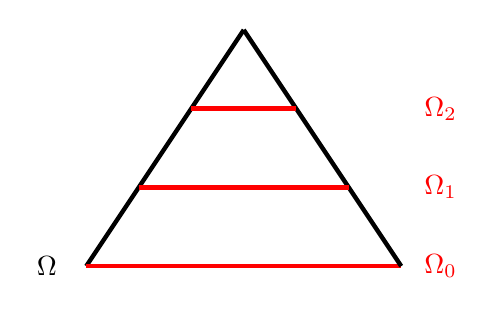
\begin{tikzpicture}
    \draw [ultra thick] (-2,0) -- (0,3);
    \draw [ultra thick, red] (-2,0) -- (2,0);
    \draw [ultra thick] (2,0) -- (0,3);
    \draw [ultra thick, red] (-4/3,1) -- (4/3,1);
    \draw [ultra thick, red] (-2/3,2) -- (2/3,2);
    \draw (2.5,0) [text=red] node {$\Omega_0$};
    \draw (2.5,1) [text=red] node {$\Omega_1$};
    \draw (2.5,2) [text=red] node {$\Omega_2$};
    \draw (-2.5,0) node {$\Omega$};
\end{tikzpicture}
\caption*{Beispiel für ein \((\Omega 1)-(\Omega 2)\)-Gebiet im \(\mathbb{R}^2\)}
\end{subfigure}%
\quad \quad \quad
\begin{subfigure}{.3\textwidth}
\centering
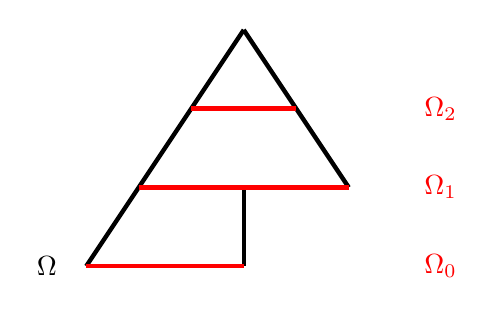
\begin{tikzpicture}
    \draw [ultra thick] (-2,0) -- (0,3);
    \draw [ultra thick] (0,0) -- (0,1);
    \draw [ultra thick, red] (-2,0) -- (0,0);
    \draw [ultra thick] (4/3,1) -- (0,3);
    \draw [ultra thick, red] (-4/3,1) -- (4/3,1);
    \draw [ultra thick, red] (-2/3,2) -- (2/3,2);
    \draw (2.5,0) [text=red] node {$\Omega_0$};
    \draw (2.5,1) [text=red] node {$\Omega_1$};
    \draw (2.5,2) [text=red] node {$\Omega_2$};
    \draw (-2.5,0) node {$\Omega$};
\end{tikzpicture}
\caption*{Beispiel für ein \((\Omega1)\)-Gebiet im \(\mathbb{R}^2\)}
\end{subfigure}
\label{fig:Omega12}
\end{figure}

Wir erinnern uns nun kurz an die Annahmen im \(\Gamma\)-Konvergenzresultat [\ref{theo4.12}, Satz 4.12] zurück. Wir haben dort angenommen, dass \(W\) (H1), (H2), (H4) erfüllt, sowie Norm-koerziv ist ((KO)). Es stellt sich dabei heraus, dass dieser Rahmen die Problemstellung \textbf{stark} vereinfacht. Der Grund ist, dass \(\sigma^*\) durch diese Annahmen einen eindimensionalen Charakter trägt (das liegt insbesondere an (H4)). Wir werden im Folgenden nur die Grundidee skizzieren, da die Details rein technisch (und dabei auch sehr aufwändig) sind und kaum zum intuitiven Verständnis unseres eigentlichen Ziels, dem \(\Gamma\)-Konvergenzresultat [\ref{theo4.12}, Satz 4.12], beitragen. Genau genommen liest sich der Zusammenhang wie folgt:\\[0.5cm]
\pgfsetfillopacity{0.1}\colorbox{generalYellow}{\begin{minipage}{16cm}{\textcolor{black}{\pgfsetfillopacity{1}}{\label{theo4.18}}}
\textbf{Satz 4.18 (\cite{ContiTwoGradientPhase}[Proposition 5.3]):} Unter eben aufgeführten Annahmen an \(W\) gilt:
\begin{equation}
    \sigma^* = \sigma^*_a = \sigma,
\end{equation}
wobei
\begin{equation}
    \sigma = \inf \{ \int_{[-L,L]} W(0,g(s)) + |\frac{dg(s)}{ds}|^2 \,d\lambda^1(s) \, | \, L > 0, \, g \in PC^1([-L,L]), \, g(L) = -g(-L) = a\}.
\end{equation}
\end{minipage}}

\textsc{Beweisidee:}
\begin{enumerate}
    \item Setze \(\{\epsilon_h\} \subset \mathbb{R}^+, \, \{u_h\} \subset W^{2,2}(Q_1,\mathbb{R}^N)\) mit \(\epsilon_h \to 0^+\) fest. (KO) sichert dann die Existenz von:
    \begin{equation}
        \forall t_k \in Q_1 \, \exists C > 0 \, : \, \sup_{k \in \mathbb{N}} |u'(t_k)| \leq C.
    \end{equation}
    Durch die Hölder-Ungleichung und (H1), sowie (H2) erhalten wir dann die gleichmäßige Beschränktheit für zulässige Folgen in \(\sigma^*_a\) in \(W^{1,\infty}(Q_1,\mathbb{R}^N)\). Per Dualität erhalten wir schwache Konvergenz in \(W^{1,1}(Q_1,\mathbb{R}^N)\). 
    \item Indem wir eine p-kompatible Koerzivitätsbedingung in (KO) wählen, erhalten wir dann auch, dass 
    \begin{equation}
    \begin{array}{l}
        \sigma^*_a = \inf \{\liminf_{h \to \infty} \int_{Q_1} \frac{W(0,u'_h)}{\epsilon_h} + \epsilon_h |u^{''}_h|^2 \,d\lambda^1(t) \, | \, \epsilon_h \to 0^+, \, u_h \in W^{2,2}(Q_1, \mathbb{R}^N), \\ 
        u_h \to |t|a \text{ in } W^{1,p}(Q_1, \mathbb{R}^N)\}
    \end{array}
    \end{equation}
    gilt.
    \item Unter der Hinzunahme von (H4), erhält man mit dem Lemma von Fatou und (2) die Behauptung in einem lokalen Fall.
    \item Schließlich ist die eindimensionale Charakterisierung auch für den "globalen" Fall zu zeigen, den man erhält, indem man die lokalen \(\sigma\) aus (3) mittels \(PC^1\)-Kurven \(g\) zu \(\sigma\) "zusammenbaut", i.e. man betrachtet:
    \begin{equation}
        u_h(t) := \int_{[0,t]} v_h (s) \,d\lambda^1(s), \, v_h(t) := \begin{cases}
            -a, \text{ falls }t < -\epsilon_h L \\
            g(\frac{t}{\epsilon_h}), \text{ falls }|t| \leq \epsilon_h L \\
            a, \text{ falls }t > \epsilon_h L
        \end{cases}.
    \end{equation}
    Das ist natürlich genau so konstruiert, dass 
    \begin{equation}
        v_h \to v_0 := \begin{cases}
            -a, \text{ falls }t \leq 0 \\
            a, \text{ falls }t > 0
        \end{cases}
        \text{ in }L^p(Q_1,\mathbb{R}^N) \, \forall p \in [1,\infty[
    \end{equation}
    gilt, also insbesondere:
    \begin{equation}
        u_h \to |t|a \text{ in }W^{1,p}(Q_1,\mathbb{R}^N).
    \end{equation}
\end{enumerate}
Für die Details verweisen wir auf \cite{ContiTwoGradientPhase} [Proposition 5.1, Corollary 5.2, Proposition 5.3]. \QEDB

Nun befinden wir uns in der Situation, das \(\Gamma\)-Limsupresultat für den \((\Omega1)-(\Omega2)\)-Fall zu beweisen:\\[0.5cm]
\pgfsetfillopacity{0.1}\colorbox{generalYellow}{\begin{minipage}{16cm}{\textcolor{black}{\pgfsetfillopacity{1}}{\label{theo4.19}}}
\textbf{Satz 4.19 (\cite{ContiTwoGradientPhase}[Theorem 5.5]):} Angenommen, \(\Omega\) erfüllt \((\Omega1)\) und \((\Omega2)\), \(W\) (H1), (H2), (KO) und (H4). Sei \(u \in W^{1,1}(\Omega,\mathbb{R}^N)\) mit \(Du \in \mathcal{BV}(\Omega,\{A,B\})\). Dann gilt für \(\{\epsilon_h\} \subset \mathbb{R}^+\) mit \(\epsilon_h \to 0^+\), \(E \subset \mathcal{M}^n(\mathbb{R}^n)\):
\begin{equation}
    \Gamma-\limsup_{h \to \infty} \mathcal{I}_{\epsilon_h} (u,\Omega) \leq \sigma^* |D \chi_E| (\Omega),
\end{equation}
wobei \(Du = (1 - \chi_E(x))A + \chi_E (x) B\) \(\lambda^n\)-f.ü.
\end{minipage}}

\textsc{Beweis:} Annahme \((\Omega1)\) validiert die Anwendung von \eqref{eq4.81}, i.e. es gilt:
\begin{equation}
    u(x) = \tilde{u}(x_n) = f_0 + a x_n - 2h(x_n)a \, \lambda^n-\text{f.ü.}
\end{equation}
mit \(h \in W^{1,\infty}(\mathbb{R}), \, h' \in \mathcal{BV}(\mathbb{R},\{0,1\})\),
\begin{equation}
    S(Du) \cap \Omega = \bigcup_{i=1}^{\infty} \Omega_{l_i},
\end{equation}
wobei \(\Omega_{l_i} := \{(x',x_n) \in \Omega \, | \, x_n = l_i\}\), \(l_i \in \mathbb{R}\).\\
\textbf{Schritt 1:} Angenommen, \(S(Du) \cap \Omega = \bigcup_{i=1}^k \Omega_{l_i}, \, k \in \mathbb{N}\) beliebig, aber fest, sowie o.B.d.A. seien \(l_i\) aufsteigend total geordnet, i.e. \(l_1 < ... < l_k\). Um die Behauptung zu beweisen, wissen wir nach [\ref{theo4.18}, Satz 4.18], dass es reicht, die Behauptung für \(\sigma\), statt \(\sigma^*\) zu zeigen. Wir wählen also jetzt in diesem Rahmen Kurven \(g_j \in PC^1([-L,L],\mathbb{R}^N)\) mit \(g_j(L) = -g_j(L) = a\), sodass
    \begin{equation}{\label{eq4.120}}
        \int_{[-L,L]} W(0,g_j(s)) + |g^{\prime}_k(s)|^2 \,d\lambda^1(s) \leq \sigma + \frac{1}{j}
    \end{equation}
    gilt. O.B.d.A. wähle \(\epsilon_h\) so klein, dass \(l_i + \epsilon_h L < l_{i+1} - \epsilon_h L\) (durch ein typisches Skalierungsargument kann man diesen Rahmen immer erzwingen) für \(i=1,...,k-1\). Definiere:
    \begin{equation}{\label{eq4.121}}
        v_{\epsilon_h,j}(s) := \begin{cases}
            g_j(-sgn(u^{\prime}(l_i - \epsilon_h L) \cdot a) \frac{s-l_i}{\epsilon_h}), \text{ falls } s \in ]l_i - \epsilon_h L, l_i + \epsilon_h L[, \, i=1,...,k \\
            \tilde{u}^{\prime}(s), \text{ sonst in }\mathbb{R}
        \end{cases},
    \end{equation}
    wobei wir \(\tilde{u}^{\prime}\) stetig auf ganz \(\mathbb{R}\) fortgesetzt haben (der dafür nötige stetige Fortsetzungsoperator existiert dank des \(C^1\)-Randes des Intervalls \(]l_1- \epsilon_h L, \, l_k + \epsilon_h L[\), vergleiche hier das klassische Sobolevresultat). Dem zugrundeliegend setzen wir dann:
    \begin{equation}
        u_{\epsilon_h,j}(x) = \tilde{u}_{\epsilon_h,j} (x_n) := \tilde{u}(l_1) + \int_{[x_n,l_1]} v_{\epsilon_h,j}(s) \,d\lambda^1(s).
    \end{equation}
    Dann gilt:
    \begin{equation}
    \begin{array}{l}
        \int_{\Omega} |Du_{\epsilon_h,j} - Du| \,d\lambda^1(x) \stackrel{(\ref{eq4.121})}{\leq} C \sum_{i=1}^k \int_{[l_i - \epsilon_h L, l_i + \epsilon_h L]}|g_j(\pm \frac{s-l_i}{\epsilon_h})| + 1 \,d\lambda^1(s) \stackrel{(*)}{\leq} \\
        2Cm \epsilon_h L + C \sum_{i=1}^k \epsilon_h \int_{[-L,L]} |g_j (t)| \,d\lambda^1(t),
    \end{array}
    \end{equation}
    wobei (*) valide ist, da gilt:
    \begin{equation}
        \lim_{s \to (l_i \pm \epsilon_h L)} |g_j(\pm \frac{s-l_i}{\epsilon_h}| \stackrel{Stet.}{=} a < 2a = |g_j(L) - g_j(-L)| \stackrel{C-S}{\leq} \int_{[-L,L]} |g^{\prime}_j(s)| \,d\lambda^1(s).
    \end{equation}
    Mit der Poincare-Ungleichung erhalten wir dann, dass
    \begin{equation}{\label{eq4.125}}
        u_{\epsilon_h,j} \stackrel{\epsilon_h \to 0^+}{\to} u \text{ in }W^{1,1}(\Omega,\mathbb{R}^N)
    \end{equation}
    gilt. Zusammengefasst erhalten wir:
    \begin{equation}
    \begin{array}{l}
        \lim_{\epsilon_h \to 0^+} \mathcal{I}_{\epsilon_h} (u_{\epsilon_h,j},\Omega) \stackrel{Def.}{=} \\
        \lim_{\epsilon_h \to 0^+} \sum_{i=1}^k \int_{\Omega \cap \{l_i + \epsilon_h L < x_n < l_{i+1} + \epsilon_h L\}} \frac{W(0,g_j(\pm \frac{x_n - l_i}{\epsilon_h}))}{\epsilon_h} + \frac{1}{\epsilon_h} |g^{\prime}_j (\pm \frac{x_n - l_i}{\epsilon_h})|^2 \,d\lambda^1(x) \stackrel{Cav.}{=} \\
        \lim_{\epsilon_h \to 0^+} \sum_{i=1}^k \int_{[l_i - \epsilon_h L, l_i + \epsilon_h L]} (\frac{W(0,g_j(\pm \frac{s - l_i}{\epsilon_h}))}{\epsilon_h} + \frac{1}{\epsilon_h} |g^{\prime}_j (\pm \frac{s - l_i}{\epsilon_h})|^2) \mathcal{H}^{n-1}(\{x \in \Omega \, | \, x_n = s\}) \,d\lambda^1(s) \stackrel{(\ref{eq4.125})}{=}\\
        \lim_{\epsilon_h \to 0^+} \sum_{i=1}^k \int_{[-L,L]} (W(0,g_j(t)) + |g^{\prime}_j(t)|^2) \mathcal{H}^{n-1}(\{x \in \Omega \, | \, x_n = \epsilon_h t + l_i \})\,d\lambda^1(t) \stackrel{(\Omega2)}{=} \\
        (\int_{[-L,L]} W(0,g_j(t)) + |g^{\prime}_j (t)|^2 \,d\lambda^1(t)) \sum_{i=1}^k \mathcal{H}^{n-1}(\Omega_{l_i}) \stackrel{(\ref{eq4.120})}{\leq} (\sigma + \frac{1}{j}) \sum_{i=1}^k \mathcal{H}^{n-1}(\Omega_{l_i}).
    \end{array}
    \end{equation}
    Betrachten wir dann \(\limsup_{j \to \infty}\), so erhalten wir die Behauptung.\\
\textbf{Schritt 2:} Angenommen, \(S(Du) \cap \Omega = \bigcup_{i=1}^{\infty} \Omega_{l_i}\). Dann erhalten wir die Behauptung limitisch aus Schritt 1, da für einen Häufungspunkt \(l\) von \(\{l_i\}\) gilt, dass \(l \in \{\alpha,\beta\}\).\\[0.2cm]
    \textit{Begründung, dass das gilt: Angenommen, das wäre falsch, so gilt für \(\Omega_l \neq \emptyset\), dass ein \(x = (x',l) \in \Omega\) existiert und \(B_{r}(x') \, \times ]l-d,l+d[ \subset \Omega\) offen (bezüglich der euklidischen Relativtopologie) für \(d \in \mathbb{N}\). Für \(i_j\) groß genug, ist auch \(B_{r}(x') \, \times \{l_{i_j}\} \subset \Omega\) offen (bezüglich der euklidischen Relativtopologie), wobei \(\{l_{i_j}\} \to l\) und damit:
    \begin{equation}
        \infty > \sum_{i=1}^{\infty} \mathcal{H}^{n-1} (\Omega_{l_i}) \geq \sum_{i_j} \mathcal{H}^{n-1}(B_{r}(x')) = \infty.
    \end{equation}
    }\\[0.2cm]
    Sei also nun wieder \(k \in \mathbb{N}\) beliebig, aber fest. Definiere:
    \begin{equation}
        U_k := \{x \in \Omega \, | \, \alpha + \delta_k < x_n < \beta - \delta_k\},
    \end{equation}
    wobei \(\delta_k \to 0^+\), also \(\{l_i\} \cap \{\alpha + \delta_k, \beta - \delta_k\} \stackrel{s.o.}{=} \emptyset\). Damit gilt \(\lambda^n(\Omega \textbackslash U_k) \stackrel{k \to \infty}{\to} 0\) und die Behauptung folgt aus Schritt 1. 
Damit ist die Behauptung gezeigt. \QEDB
%%%%%%%%%%%%%%%%%%%%%%%%%%%%%%%%%%%%%%%%%%%%%%%%%%%%%%%%%%%%%%%%%%%%%%%%%%%%
\subsection[Verbesserungen des Conti-Fonseca-Leoni Modells: Der Weg zur SO(N)-Invarianz]{Verbesserungen des Conti-Fonseca-Leoni Modells: Der Weg zur SO(\(\mathbb{N}\))-Invarianz}{\label{subsec:soninva}}
Wir erinnern nun noch einmal an die Annahmen, die im letzten Unterkapitel getroffen wurden (Definitionen wie gehabt):
\begin{itemize}
    \item (H1) \(\exists a \in \mathbb{R}^N \, \textbackslash \{0\} \, : \, A -                 B = a \otimes \nu\),
    \item (H2) W ist stetig, \(\{W = 0\} = \{A,B\}\),
    \item (H3) \(\exists C > 0 \, \forall z \in \mathbb{R}^{N \times n} \, : \,                 W(z) \geq C |z| - \frac{1}{C}\).
    \item (H4) \(W(z) \geq W(0,z_n)\) mit \(z = (z',z_n) \in \mathbb{R}^{N                      \times (n-1)} \times \mathbb{R}^N\).
\end{itemize}
Wir hatten in [\ref{prop4.11}, Proposition 4.11] begründet, dass (H1) im Allgemeinen keine große Einschränkung darstellt. Auch (H3) ist keine zu große Einschränkung, denn ohne jegliche Wachstumsschranken ist generell keine \(\Gamma\)-Konvergenz zu erwarten. Allerdings sind der zweite Teil von (H2) ((H2)-2) und (H4) sehr störend. (H2)-2 erzeugt ein starres Modell, da jegliche Oszillationen zwischen den einzelnen Potentialen komplett vernachlässigt wird. (H4) ist hierbei aber die stärkste Einschränkung, da sie eine Kontrolle durch ein eindimensionales Problem annimmt. Wir werden nun aktuelle Forschungsergebnisse aufführen, die sich mit diesen Problemen befasst haben. Dabei werden wir aber nur die neuen Ideen aufführen, Details lassen sich dann in den \\jeweiligen Quellen finden.

\subsubsection{Schritt 1: SO(2)-Invarianz nach S. Conti und B. Schweizer in \cite{conti2006rigidity}}
Wir modifizieren die Bedingungen nun also zu:
\begin{itemize}
    \item (H1)' \(\exists a \in \mathbb{R}^2 \, : \, A-QB = a \otimes \nu\),
    \item (H2)' \(W \in C(\mathbb{R}^{2 \times 2}) \, : \, (W(QF) = W(F) \, \forall F \in \mathbb{R}^{2 \times 2}, \, Q \in SO(2) \, \land \, \{W = 0\} = K := SO(2)A \cup SO(2)B)\),
    \item (H3)' \(c_1 d_{Fr}^2(F,K) \leq W(F) \leq c_2 d_{Fr}^2(F,K)\) (Fr steht hier für Frobenius; die Metrik ist also die von der Frobenius-Norm induzierte.),
\end{itemize}
wobei \(det \, A > 0, \, det \, B > 0, \, c_1, \, c_2 > 0\). S. Conti und B. Schweizer bewiesen auf dieser Grundlage folgendes Theorem:\\[0.5cm]
\pgfsetfillopacity{0.1}\colorbox{generalYellow}{\begin{minipage}{16cm}{\textcolor{black}{\pgfsetfillopacity{1}}{\label{theo4.20}}}
\textbf{Satz 4.20 (\cite{conti2006rigidity}[Theorem 3.1]):} Angenommen, \(\Omega \subset \mathbb{R}^2\) ist ein strikt sternförmiges, beschränktes Lipschitz-Gebiet, in dem (H1)', (H2)' und (H3)' erfüllt sind. Dann gilt für \(u \in W^{1,1}(\Omega, \mathbb{R}^2)\):
\begin{equation}
    \Gamma-\lim_{\epsilon \to 0} \mathcal{I}_{\epsilon} (u,\Omega) = \mathcal{I}_0(u,\Omega) := \begin{cases}
        \sigma^* \mathcal{H}^1(S(Du) \cap \Omega), \text{ falls } Du \in \mathcal{BV}(\Omega,K) \\
        \infty, \text{ sonst}
    \end{cases},
\end{equation}
wobei
\begin{equation}
    \sigma^* := \inf \{\liminf_{h \to \infty} \mathcal{I}_{\epsilon_h} (u_h,Q_{\nu}) \, | \, \epsilon_h \to 0, \, u_h \to u_0 \text{ in }L^1(Q_2,\mathbb{R}^N)\}
\end{equation}
und
\begin{equation}
    Du_0 := \begin{cases}
        A, \text{ falls } x \cdot \nu > 0 \\
        QB, \text{ falls } x \cdot \nu < 0
    \end{cases}.
\end{equation}
\end{minipage}}

\textsc{Beweisidee:} Wie üblich benötigen wir wieder ein Kompaktheits- \(\Gamma\)-liminf und \(\Gamma\)-limsup Resultat:
\begin{itemize}
    \item \textbf{Kompaktheit:} Wir halten zunächst fest (das Ursprungsresultat ist in \cite{ball1984w1} zu finden): Ist eine Lebesgue-integrable Funktion \(g : \mathbb{R} \to \mathbb{R}\) periodisch auf einem Ball \(B_r(x)\) durch eine lokal Lebesgue-integrable Funktion \(h:\mathbb{R}^n \to \mathbb{R}\) fortgesetzt, so gilt für eine Borelmenge \(E\), sowie
    \begin{equation}
        w_j := h(jx),
    \end{equation}
    dass \(w_j\) ein Young-Maß \(\vartheta_x \in \mathcal{Y}(\Omega,\mathbb{R}^N)\) erzeugt, für das gilt:
    \begin{itemize}
        \item \(\int_{\mathbb{R}} g \,d\vartheta_x = \int_{B_r(x)} g(h(y)) \,d\lambda^n(y)\),
        \item \(\vartheta_x(E) = \lambda^n(B_r(x) \cap h^{-1}(E))\).
    \end{itemize}
    Damit ist klar, dass gilt:
    \begin{equation}
        \int_{B_r(x)} \vartheta_x(SO(n)B) \,d\lambda^n(x) = \lambda^n(B_r(x) \cap E).
    \end{equation}
    Der Träger von dem für unseren Rahmen erzeugte Young-Maß \(\vartheta_x\) ist wieder in einer kompakten Menge, weshalb wir das Kompaktheitsresultat schließen können, wenn wir zeigen, dass für Lebesgue-Punkte \(x_0\) der Dichte 0 zeigen, dass \(Du_0(x_0) \in SO(n)A\) gilt (da wir nach [\ref{lem2.3}, Lemma 2.3] wissen, dass für \(L^1\)-Funktionen \(\lambda^n\)-f.a. Punkte der Funktion Lebesgue-Punkte sind). Kurz gesagt ist das korrekt, da die Hilfsfunktion
    \begin{equation}
        \phi(z) := ||z||^n_{Fr} - n^{n/2} det \,z
    \end{equation}
    polykonvex ist (valide, da für \((2 \times 2)\)-Matrizen die Determinante polykonvex ist (aber \textbf{nicht} konvex!)).
    \item \textbf{\(\Gamma\)-Liminf:} Da wir für die Wachstumsbeschränkung nach unten den nahezu identischen Rahmen vorliegen haben, ist der Beweis fast identisch zu dem von [\ref{theo4.15}, Satz 4.15]. Die Idee ist es, Rechtecke zwischen den "Schnittstellen" (also an dem Übergang von Phase A zu Phase B bzw. vice versa) auf \(S(Du)\) zu betrachten und schlussendlich die Unabhängigkeit der Größe der Rechtecke zu zeigen.
    \item \textbf{\(\Gamma\)-Limsup:} Wie immer ist dieser Schritt der mit Abstand schwierigste. Die Idee ist hier, um
    \begin{equation}
        \mathcal{I}_{\epsilon_h}(u_h,\Omega) \to \mathcal{I}_0(u_0,\Omega)
    \end{equation}
    für \(u_h \to u_0\) zu erhalten, limitische Funkten zu betrachten, die endlich viele Schnittstellen besitzen, die nicht auf dem Rand liegen (diese Approximation ist valide, da sie dicht in \(\Omega\) liegt). \QEDB
\end{itemize}

\subsubsection{Schritt 2: SO(\(\mathbb{N}\))-Invarianz nach E. Davoli und M. Friedrich in \cite{davoli2020two}}
Als nächsten Schritt bewiesen E. Davoli und M. Friedrich den allgemeinen Fall, jedoch unter Hinzunahme eines anisotropischen Regularitätstermes, i.e. das Energiefunktional
\begin{equation}
    \mathcal{E}_{\epsilon,\eta} := \begin{cases}
        \mathcal{I}_{\epsilon} (u,\Omega) + \eta^2 \int_{\Omega} ||D^2 u||_{Fr}^2 - |\partial_n^2 u|^2 \,d\lambda^n(x), \text{ falls }u \in W^{2,2}(\Omega,\mathbb{R}^n) \\
        \infty, \text{sonst}
    \end{cases},
\end{equation}
wobei \(\eta > 0\). Als zweite Einschränkung modifizieren wir jetzt noch (H1) zu:
\begin{itemize}
    \item (H1) \(\exists a \in \mathbb{R}^n \textbackslash \{0\} : B - A = a e_n \otimes e_n\).
\end{itemize}
Wir haben bereits in [\ref{prop4.11}, Proposition 4.11] gesehen, dass (H1) keine allzugroße Einschränkung darstellt, so auch hier. Wir führen nun die wesentlichen neuen Ideen auf zu dem Conti-Resultat [\ref{theo4.13}, Satz 4.13]. Diese beschränken sich rein auf den Beweis des \(\Gamma\)-Limsup. Im Folgenden nehmen wir stets für die Phasenseperation die Wachstumsschranke:
\begin{equation}
    \int_{\Omega} W(Du) \,d\lambda^n(x) \leq C \epsilon^2, \, C > 0
\end{equation}
an. Bisherige Resultate befassten sich mit einem komplett starren Modell ([\ref{theo4.12}, Satz 4.12]) oder nahmen nur Rücksicht auf \textbf{eines} der beiden Potentiale. Letzteres umfasst z.B. Modelle mit stark inkompatiblen Potentialen (\cite{de2006simple}, \cite{chaudhuri2004rigidity}; für diese Arbeit irrelevant, da hier offensichtlich \textbf{keine} Phasentrennung entsteht (das sieht man sogar mathematisch: für \(\epsilon \ll 1\) ist \(Du \sim F \in \mathbb{R}^{n \times n}\))). Um beide (kompatiblen) Potentiale simultan modellieren zu können, benötigen wir eine Art "Indikator", um dynamisch die "aktive" Phase jeweils zu betrachten. Genau solch einen "Phasen-Indikator" führten E. Davoli und M. Friedrich in \cite{davoli2020two} ein: Wir werden diesen im Folgenden mit \(\mathcal{M} \in \mathcal{BV}(\Omega, \{A,B\})\) bezeichnen. Damit wir das Conti-\(\Gamma\)-Konvergenz Resultat [\ref{theo4.20}, Satz 4.20] in allgemeiner Dimension erreichen können, müssen wir einen passenden Rahmen finden, der uns die korrekten sogenannten "Starrheits Abschätzungen" (Englisch: rigidity estimates) liefert. Korrekt heißt in dem Zusammenhang eine Abschätzung der Form:
\begin{equation}{\label{eq4.138}}
    \exists R \in SO(n) \, : \, ||Du - R\mathcal{M}||_{L^2(\Omega)} \leq C \epsilon.
\end{equation}

\textbf{Bemerkung:} Die Ordnung \(\epsilon\) ist wichtig, da Verzerrung in fest-fest Phasenübergängen in den allermeisten Fällen von genau dieser Ordnung auftritt! Beispielsweise haben R. Jerrard und A. Lorent in \cite{jerrard2013multiwell} unter der Annahme von:
\begin{equation}{\label{eq4.139}}
    ||D^2 u||_{L^1(\Omega)} \leq C_1, \, 0 < C_1 < 1,
\end{equation}
gezeigt, dass die Folgende Abschätzung gilt:
\begin{equation}
    ||Du - R\{A,B\}||_{L^2(\tilde{\Omega})} \leq C \sqrt{\epsilon},
\end{equation}
wobei \(\tilde{\Omega} \subset \Omega\). Das Resultat kann im Allgemeinen \textbf{nicht} auf ganz \(\Omega\) erweitert werden; Grund hierfür sind hier nicht ausgeschlossene, mögliche Phasenübergänge nahe des Randes von \(\Omega\). \(C_1\) ist hier derart klein in \eqref{eq4.139} gefordert, um die Dominanz der \(\{A,B\}\)-Phasenregion zu garantieren. Die Ordnung der Abschätzung passt aber nicht und noch schlimmer: es kann sogar gezeigt werden, dass diese Schranke scharf ist, siehe \cite{davoli2020two}[Remark 3.9].

Wir geben hier nun das entscheidende Starrheits Resultat an, das gleichzeitig auch zeigt, warum der zusätzliche \(\eta\)-Stabilitätsterm in \(\mathcal{E}_{\epsilon, \eta}\) unter ähnlichen Annahmen wie im Conti-Fall, i.e. wir nehmen an, dass gilt:
\begin{itemize}
    \item (H1)' : Siehe oben;
    \item (H2) : \(W : \mathbb{R}^{n \times n} \to [0,\infty[\) ist stetig;
    \item (H3) : \(W(RF) = W(F)\) für alle \(R \in SO(n), \, F \in \mathbb{R}^{n \times n}\);
    \item (H4) : \(W(\mathbb{1}) = W(diag(1,...,1,1 + \kappa))\) für \(\kappa > 0\);
    \item (H5) : \(\exists C_2 > 0 \, \forall F \in \mathbb{R}^{n \times n} \, : W(F) \geq C_2 d_{Fr}^2(F,SO(n)\{A,B\})\),
\end{itemize}
nötig ist:\\[0.5cm]
\pgfsetfillopacity{0.1}\colorbox{generalYellow}{\begin{minipage}{16cm}{\textcolor{black}{\pgfsetfillopacity{1}}{\label{theo4.21}}}
\textbf{Satz 4.21 (\cite{davoli2020two}[Theorem 3.1]):} Angenommen, (H1)', sowie (H2) - (H5) gelten. Wir unterscheiden:
\begin{enumerate}
    \item \textbf{(Dimension 2):} Sei \(\Omega\) ein beschränktes, einfach zusammenhängendes Lipschitz Gebiet in \(\mathbb{R}^2\), \(\eta \geq \epsilon > 0\). Dann existiert eine Konstante \(C = C(\Omega,\kappa,C_2)\) > 0, sodass für alle \(u \in W^{2,2}(\Omega,\mathbb{R}^2)\) ein \(R \in SO(2)\) existiert mit:
    \begin{equation}
        ||Du - R \mathcal{M}||_{L^2(\Omega)} \leq C \epsilon \sqrt{\mathcal{E}_{\epsilon,\eta}(u)} + C (\frac{\epsilon}{\eta} + \frac{\epsilon^{1/2}}{\eta^{3/2}}) \mathcal{E}_{\epsilon,\eta}(u).
    \end{equation}
    \item \textbf{(Dimension \(\geq 3\)):} Sei \(\Omega\) ein beschränktes Lipschitz Gebiet in \(\mathbb{R}^n\) mit \(n \geq 3\). Sei zudem \(p \in [1,2]\), \(p \neq \frac{n}{n-1}\), \(\eta \geq \epsilon > 0\). Dann existiert für alle \(\tilde{\Omega} \in \overline{K}(\Omega)\) eine Konstante \(C = C(\Omega, \tilde{\Omega}, \kappa, p, C_2) > 0\), sodass für alle \(u \in W^{2,2}(\Omega,\mathbb{R}^n)\) ein \(R \in SO(n)\) existiert mit:
    \begin{equation}
        ||Du - R \mathcal{M}||_{L^p(\tilde{\Omega})} \leq C \epsilon \sqrt{\mathcal{E}_{\epsilon,\eta}(u)} + C ((\frac{\epsilon}{\eta} + \frac{\epsilon^{1/2}}{\eta^{3/2}}) \mathcal{E}_{\epsilon,\eta}(u))^{\theta},
    \end{equation}
    wobei \(\theta := \min \{1,\frac{n}{p(n-1)}\}\).
\end{enumerate}
In beiden Fällen gilt zudem:
\begin{equation}
    |D\mathcal{M}|(\Omega) \leq C \mathcal{E}_{\epsilon,\eta}(u).
\end{equation}
\end{minipage}}

\textbf{Bemerkung:} Auch in (2) kann das Resultat im Allgemeinen wieder nicht auf ganz \(\Omega\) erweitert werden. Der Beweis nutzt diesen Aspekt in dem Sinne aus, dass er per Approximation die Aussage auf einer Überdeckung mit (bezüglich der euklidischen Relativtopologie) offenen Quadern zeigt (diese endliche Teilüberdeckung ist möglich, da \(\mathbb{R}^n\) total beschränkt ist und in \(\mathbb{R}^n\) alle Normen äquivalent sind). Generell sieht man an dem Resultat schon auftretende Probleme in höheren Dimensionen als 2; wir werden später in \ref{sec:gendim} noch genauer darauf eingehen, warum das Verallgemeinern der Conti-Beweis-Strategie in [\ref{theo4.20}, Satz 4.20] alles andere als einfach ist.
%%%%%%%%%%%%%%%%%%%%%%%%%%%%%%%%%%%%%%%%%%%%%%%%%%%%%%%%%%%%%%%%%%%%%%%%%%%%%%%%%%%%%%%%%%%%%%%%%%%%%%%%%%%%%%%%%%%%%%%%%%%%%%%%%%%%%%%%%%%%
\section{Physikalischer Exkurs: Doppelter Potentialtopf}{\label{sec:exwell}}
Dieser Exkurs beschäftigt sich mit der Physik hinter dem doppelten Potentialtopf. Quantenmechanische Grundlagen werden hierfür vorausgesetzt; für das Verständnis der Arbeit ist dieser Exkurs allerdings rein optional.\\

Wir erinnern uns an den unendlichen Potentialtopf aus der Quantenmechanik und modifizieren diesen nun. Diesem ist geschuldet, dass wir zwei nicht homogene Stoffe vorliegen haben, weshalb wir im Modell quantenmechanisch zwei "aneinanderhängende" Potentialtöpfe mit Tunneling Effekten betrachten müssen, i.e. Teilchen tunneln durch die Barriere der beiden Potentiale. Physikalisch ist der Übergang zwischen den beiden Stoffen deshalb nicht-trivial und die Eigenenergien der Potentialtöpfe werden durch Tunneling Effekte bedeutend beeinflusst. Als Beispiel werden wir nun das Problem aus \cite{DoubleWellBerdecia} betrachten:\\
Wir betrachten ein Teilchen der Masse m mit Potential
\begin{equation}
    V : \mathbb{R} \to \mathbb{R}, \, V(x) := \alpha x^4 - \beta x^2 + \gamma \, \, \forall \alpha > 0 \, \forall \beta > 0,
\end{equation}
wobei \(\gamma = \frac{\beta^2}{4 \alpha}\) die Höhe der Potentialbarriere darstellt. In diesem Rahmen lässt sich die Schrödinger-Gleichung schreiben als
\begin{equation}
    (\mathbb{H} - \eta) \Psi(x) = 0,
\end{equation}
wobei der Hamilton Operator \(\mathbb{H}\) und \(\eta\) hier definiert sind als:
\begin{equation}
    \mathbb{H}x := \frac{d^2}{dx^2} - (\frac{2m}{\hbar^2})V(x), \, \eta := -(\frac{2mE}{\hbar^2})
\end{equation}
mit der Energie E. Graphisch entspricht dieser Rahmen folgender Vorstellung:
\begin{figure}[label={fig:dwp}, caption={Ein Beispiel für einen eindimensionalen Doppelpotentialtopf in symmetrischer Form \cite{DoubleWellBerdecia}}]
    \includegraphics[scale=0.5]{figures/DoubleWellPot.pdf}
\end{figure}

Unser Ziel ist es im nächsten Kapitel, als Anwendung ein variationelles Modell für Lithium-Ionen Akkus (genauer: LiFePO\(_4\) (Lithium-Eisenphosphat) Akkumulatoren) zu betrachten. Bevor wir diesbezüglich das variationelle Modell mathematisch unter die Lupe nehmen, stellt sich aus diesem Exkurs zunächst einmal die Frage heraus: Wie überträgt sich hier die Rolle des doppelten Potentialtopf physikalisch? H. Federmann, M. Fleck und H. Emmerich von der Universität Bayreuth haben sich genau diese Frage gestellt und ihre Ergebnisse in \cite{LiFedermann} festgehalten:\\
Der hier benutzte Ansatz wird als Phasenfeldmethode bezeichnet. Sie ist die physikalische Beschreibung der mathematischen Theorie der Phasenübergänge. In einem Lithium-Ionen Akku findet ein Phasenübergang an der Elektrode statt: Je nachdem, ob Lithium deinsertiert oder insertiert wird, entstehen verschiedene Phasen. Den Prozess der Desinsertion und Insertion kann man sich folgendermaßen vorstellen:
\newpage
\begin{figure}[label={fig:lidesint}, caption={Der Prozess der Lithium Desinsertion/Insertion graphisch dargestellt \cite{LiFedermann}}]
    \includegraphics[scale=0.5]{figures/LithiumAkkus.pdf}
\end{figure}

Die Verbindung bezüglich des doppelten Potentialtopfs ist dann wie folgt:\\
Sei \(\Phi : \mathbb{R}^n \times \mathbb{R} \to \{0,1\}, \, (x,t) \mapsto \Phi(x,t)\) das Phasenfeld, welches den Wert 0 für Lithium arme Phasen und 1 für Lithium reiche Phasen annimmt. Die Grenzflächenenergie wird dann beschrieben durch:
\begin{equation}
    \mathcal{E}_g (\Phi) = \frac{3 \mathcal{E}_o b}{2} (\nabla \Phi)^2 + \frac{6 \mathcal{E}_o}{b} W(\Phi),
\end{equation}
wobei \(W(\Phi) = \Phi^2(1-\Phi)^2\) dem zugehörigen doppelten Potentialtopf entspricht und \(\mathcal{E}_o\) die Oberflächenenergie, sowie b die Breite der Grenzfläche darstellen.
		\chapter[Anwendung: Variationelles Modell von LiFePO4 Akkumulatoren]{Anwendung: Variationelles Modell von LiFePO\(_4\) Akkumulatoren}{\label{ch:battery}}
Inspiration: \cite{Stinson_2021} \\
Lithium-Akkumulatoren haben in den letzten Jahrzehnten eine revolutionäre Veränderung in der Energiespeicherindustrie bewirkt. Diese wiederaufladbaren Batterien sind bekannt für ihre hohe Energiedichte, lange Lebensdauer und schnelle Ladezeiten, wodurch sie zu einer beliebten Wahl für eine Vielzahl von Anwendungen geworden sind. Lithium-Batterien basieren auf der Verwendung von Lithiumverbindungen als Elektrolyt und Elektrodenmaterialien, was zu einer effizienten und zuverlässigen Stromversorgung führt. Sie werden in Geräten wie Mobiltelefonen, Laptops, Elektrofahrzeugen und sogar in Energiespeichersystemen für erneuerbare Energien eingesetzt. Diese Batterien haben eine große Bedeutung für die Energiewende und tragen zur Reduzierung von Treibhausgasemissionen und der Abhängigkeit von fossilen Brennstoffen bei. Die kontinuierliche Forschung und Entwicklung im Bereich der Lithium-Batterien zielt darauf ab, ihre Leistungsfähigkeit weiter zu verbessern und gleichzeitig Kosten zu senken, um ihre Anwendbarkeit in verschiedenen Branchen zu erweitern.
\section{Physikalische Einführung}{\label{sec:phyintrobatt}}
\subsection[Aufbau von LiFePO4 Akkumulatoren]{Aufbau von LiFePO\(_4\) Akkumulatoren}{\label{subsec:strucbatt}}
Quelle für dieses Unterkapitel: \cite{LiAkkuSkillLync} \\
Lithium-Akkumulatoren bestehen in der Regel aus mehreren grundlegenden Komponenten, die zusammenarbeiten, um elektrische Energie zu speichern und abzugeben. Der grobe Aufbau liest sich wie folgt:
\begin{itemize}
    \item \textbf{Anode:} Die Anode ist die negative Elektrode der Batterie und besteht typischerweise aus Graphit (Graphit ist das (Stand September 2023) optimale Material bezüglich elektrischer Leitfähigkeitsmaximierung und gleichzeitiger Kostenminimierung) oder einem anderen kohlenstoffbasierten Material. Beim Entladen der Batterie gibt die Anode Lithium-Ionen ab.
    
    \item \textbf{Kathode:} Die Kathode ist die positive Elektrode der Batterie und besteht aus einer Verbindung, die Lithium-Ionen aufnimmt, wenn die Batterie aufgeladen wird. Die Kathode kann aus verschiedenen Materialien bestehen, wie beispielsweise Lithiumkobaltoxid (LiCoO\(_2\)), Lithiumeisenphosphat (LiFePO\(_4\)) oder Lithiumnickel-Mangan-Kobaltoxid (LiNiMnCoO\(_2\)) (wir werden - wie der Titel des Kapitels bereits suggeriert - im Folgenden den LiFePO\(_4\)-Fall betrachten).

    \item \textbf{Elektrolyt:} Der Elektrolyt ist eine leitfähige Substanz, die es Lithium-Ionen ermöglicht, zwischen der Anode und der Kathode zu wandern. In Lithium-Ionen-Batterien wird häufig ein organisches Lösungsmittel mit Lithiumsalzen als Elektrolyt verwendet. Es gibt auch feststoffbasierte Elektrolyte, die anstelle von flüssigen Elektrolyten eingesetzt werden können.

    \item \textbf{Separator:} Der Separator ist eine dünne poröse Membran, die zwischen der Anode und der Kathode platziert wird, um einen direkten Kontakt zwischen den beiden Elektroden zu verhindern und Kurzschlüsse zu vermeiden. Der Separator erlaubt jedoch den Durchtritt von Lithium-Ionen.

    \item \textbf{Gehäuse:} Das Gehäuse umgibt die internen Komponenten der Batterie und schützt sie vor äußeren Einflüssen. Es besteht in der Regel aus einem stabilen Metall oder Kunststoff.
\end{itemize}

\begin{figure}[label={fig:liakkuaufbau}, caption={Aufbau eines Lithium-Akkumulators \cite{LyncPicLi}}]
    \includegraphics[scale=0.6]{figures/mceclip0_1642665078.png}
\end{figure}
\subsection{Beschreibung von Tensoren verschiedener Ordnungen in der Physik}{\label{subsec:tensorphy}}
Inspiration: \cite{NasaTensors} \\
Um einen Lithium-Akkumulator mathematisch erfassen zu können, werden wir aufgrund der auftretenden Elastizität auf die Theorie der Tensoren zurückgreifen müssen. Intuitiv gesprochen entspricht ein Tensor der Ordnung n einer "n-dimensionalen Matrix". Die Vorstellung von Matrizen in "hintereinanderliegenden" Ebenen ist deshalb eine gute erste Intuition. Dabei erinnern wir daran, dass wir für einen \((r,s)\)-Tensorraum mit \(r,s \in \mathbb{N}\), die Summe \(r+s =: n\) als Ordnung bezeichnen. Wir beschreiben nun Anwendungen aus der Physik:
\begin{itemize}
    \item \textbf{Tensoren der Ordnung 0 (Skalare):} Diese stellen lediglich eine einzelne Zahl dar. In der Physik wird er demnach verwendet, um Größen wie Masse, Temperatur oder Energie darzustellen.

    \item \textbf{Tensoren der Ordnung 1 (Vektoren):} Diese enthalten die Richtung und den Betrag einer physikalischen Größe. In der Physik werden diese zum Beispiel zur Darstellung von Geschwindigkeit und Kraft verwendet.

    \item \textbf{Tensoren der Ordnung 2:} Diese können durch eine Matrix repräsentiert werden. Beispielsweise wird der Spannungstensor in der Festkörpermechanik verwendet, um die Spannungsverteilung in einem deformierten Festkörper zu beschreiben. Der metrische Tensor in Einstein's allgemeiner Relativitätstheorie besitzt ebenfalls die Ordnung 2.

    \item \textbf{Tensoren der Ordnung 3:} Diese werden in der Kontinuumsmechanik verwendet, um komplexe Verformungs- und Spannungszustände zu beschreiben. In der Strömungsmechanik werden sie verwendet, um die turbulenten Eigenschaften von Strömungen zu analysieren.

    \item \textbf{Tensoren der Ordnung 4:} Diese werden in der Kontinuumsmechanik verwendet, um Elastizität zu beschreiben. Wir werden deshalb für die Modellierung des Lithium-Akkumulators auf diese Art von Tensor im Folgenden zurückgreifen. Eine weitere wichtige Anwendung finden diese in der Data Science, da diese "multilayer networks" beschreiben.
    
    \item \textbf{Tensoren höherer Ordnung:} Diese werden zum Beispiel in der Quantenmechanik verwendet, um die Wechselwirkungen zwischen mehreren Teilchen zu beschreiben.
\end{itemize}
%%%%%%%%%%%%%%%%%%%%%%%%%%%%%%%%%%%%%%%%%%%%%%%%%%%%%%%%%%%%%%%%%%%%%%%%%%%5
\section{Analytische Betrachtung von Akkumulatoren: Akkumulatoren nahe des Gleichgewichtszustandes}{\label{sec:anabatt}}
Bevor wir die mathematische Beschreibung dieses Problems präsentieren können, erinnern wir kurz an folgendes Resultat aus der linearen Algebra zurück:\\
Betrachte eine Matrix \(M \in \mathbb{R}^{n \times m}\). Dann kann man jede solche Matrix in ihren symmetrischen und anti-symmetrischen Anteil zerlegen, i.e. es gilt:
\begin{equation}
    M = \frac{M + M^T}{2} + \frac{M - M^T}{2}.
\end{equation}
Dabei sei angemerkt, dass diese Darstellung eindeutig ist. Im Folgenden werden wir den symmetrischen Anteil der Jakobi-Matrix benötigen. Wir setzen also in gängiger Notation fest:
\begin{equation}
    u: \Omega \to \mathbb{R}^n, \, e(u):= \frac{Du + (Du)^T}{2}.
\end{equation}
Wir werden in diesem Unterkapitel der Arbeit von K. Stinson aus dem Jahr 2021 in \cite{Stinson_2021} folgen, betrachten also im Folgenden den Spezialfall \(\Omega \subset \mathbb{R}^2\) (der Grund hiefür ist, dass zu dem Zeitpunkt der Forschung in dessen Dokument die Gültigkeit des \(\Gamma\)-Konvergenz Resultats von [\ref{theo4.20}, Satz 4.20] nur für Dimension 2 bekannt war; K. Stinson übertrug die dortig benutzte Beweismethode auf das Akkumulator Modell). Für das vorliegende konkrete Anwendungsbeispiel liegt das Doppelpotential \(W\) in folgender Form vor:
\begin{equation}
    \tilde{W}(y) := \omega y(1-y) + k_B T (y \, log(y) + (1-y) log(1-y)), \forall y \in [0,1],
\end{equation}
wobei \(k_B\) die Boltzmann-Konstante, \(T\) den Temperaturwert (in Kelvin) und \(\omega \in \mathbb{R}\) die Mischungsenthalpie (Enthalpie entspricht informell gesprochen dem Wärmeinhalt) beschreibt. Das zugehörige Energie-Funktional trägt dann folgende Darstellung:
\begin{equation}{\label{eq5.4}}
\begin{array}{l}
\mathcal{I}_{\epsilon} : W^{1,2}(\Omega,\mathbb{R}^2) \, \times \, W^{1,2}(\Omega,[0,1]) \to \mathbb{R} \cup \{\infty\}, \\
    \begin{cases} \mathcal{I}_{\epsilon} (u,c,\Omega) := \int_{\Omega} \frac{1}{\epsilon} W(c) + \epsilon |\nabla c|^2 + \frac{1}{\epsilon} \mathcal{C} (e(u) - c e_0) \, : \, (e(u) - c e_0))\,d\lambda^2(x), \text{ falls }(u,c) \in \mathcal{A} \\
    \infty, \text{ sonst,}
    \end{cases}
\end{array}
\end{equation}
wobei 
\begin{itemize}
    \item \(\mathcal{A} := W^{1,2}(\Omega,\mathbb{R}^2) \, \times \, W^{1,2}(\Omega,[0,1])\),
    \item \(e_0 \in \mathbb{R}^{2 \times 2}\) die "Gitterfehlanpassung" (Engl. "lattice misfit"),
    \item \(W(y) := \tilde{W}(y) - \min_{\alpha \in [0,1]} \tilde{W}(\alpha) \, \forall y \in [0,1]\),
    \item \(c : \Omega \to [0,1]\) die normalisierte Lithium-Ionen-Dichte,
    \item \(u : \Omega \to \mathbb{R}^2\) die Materialverformung (Engl. "material displacement"),
    \item \(\mathcal{C} : \mathbb{R}^{2 \times 2} \to \mathbb{R}^{2 \times 2}_{sym}\) einen symmetrisch, positiv definiten Stiffness-Tensor vierter Ordnung mit 
    \begin{equation}
        \mathcal{C}(z) \, : \, z > 0 \, \forall z \in \mathbb{R}^{2 \times 2}_{sym} \text{ mit } z \neq 0
    \end{equation}
    beschreiben.
\end{itemize}
Bevor wir uns wieder dem \(\Gamma\)-Konvergenzresultat zuwenden, stellt sich zunächst die Frage, ob wir für \eqref{eq5.4} dieses mal einen allgemeinen Minimierer erwarten können. Wir prüfen hierfür die Bedingungen der direkten Methode [\ref{theo2.8}, Satz 2.8] im schwachen Sinne nach:
\begin{enumerate}
    \item Da \(\mathcal{A}\) schwach abgeschlossen ist (\textit{Dafür erinnern wir an das wohlbekannte Resultat, dass für \(p \in ]1,\infty[\) \(L^p(\Omega,\mathbb{R}^m)\) gleichmäßig konvex ist. Betrachte dann (angepasste Version von \cite{marcellan2018weighted}[Theorem 4.2]):
    \begin{equation}
        T : W^{1,p}(\Omega,\mathbb{R}^m) \to L^p(\Omega,\mathbb{R}^m), T(u) := \{D^{\alpha}u\}_{|\alpha| \leq 1}.
    \end{equation}
    Dieser Operator ist eine (bezüglich der Norm-Topologie) abgeschlossene und isometrische Einbettung, woraus folgt, dass \(W^{1,p}(\Omega,\mathbb{R}^m)\) ebenfalls gleichmäßig konvex ist als (bezüglich der Norm-Topologie) abgeschlossener Unterraum von \(L^p(\Omega,\mathbb{R}^m)\), insofern \(|\alpha| \leq 1\) gilt. Nach dem Lemma von Mazur ist \(W^{1,p}(\Omega,\mathbb{R}^m)\) damit als konvexe Menge auch schwach abgeschlossen (aus diesem Argument wird auch klar, warum in Anwendungsdokumenten in der Variationsrechnung niemand diese Bedingung nachprüft).}), genügt es, dass wir die Koerzivität von \(\mathcal{I}_{\epsilon}\) nachprüfen. Ohne weitere Annahmen an den Integranden von \(\mathcal{I}_{\epsilon}\) ist offensichtlich \(\mathcal{I}_{\epsilon}\) im Allgemeinen nicht koerziv. Wir werden darauf in \ref{sec:regumini} genauer eingehen.
    \item Konvexität des Integranden können wir im Allgemeinen \textbf{nicht} erwarten, da mittels physikalischer Annahmen, die wir an \(W\) setzen, \(W\) nicht konvex sein kann (Physikalisch ist zu erwarten, dass \(W(R) = 0\) gilt für alle \(R \in SO(N)\) (da deformationsfrei) und \(W(S) = \infty\) für alle \(S\) mit \(det (S) = 0\) (da singuläre Komprimierung)). Überlegungen zur Polykonvexität sind aber durchaus valide; für optimale Bedingungen an den Integranden von \(\mathcal{I}_{\epsilon}\) ist es aber natürlich besser, gleich nach quasikonvexen Bedingungen zu suchen. Dies ist in der Theorie ein valider Weg, der in der Praxis allerdings sehr schwierig zu lösen ist. Wir werden deshalb in \ref{sec:regumini} einen Existenzbeweis mittels zugehöriger Euler-Lagrange Gleichungen aufführen.
\end{enumerate}
Vergleicht man die Situation mit der aus früheren Kapiteln, so wird klar, dass eigentlich nur interessant ist, wie wir den Tensor \(\mathcal{C}\) "kontrolliert" bekommen. Für die restlichen Details verweisen wir dann auf das Dokument \cite{Stinson_2021}. Wir treffen in diesem Rahmen folgende Annahmen:
\begin{itemize}
    \item (H1) \(\mathcal{C}(z) \, : \, z > 0 \, \forall z \in \mathbb{R}^{2 \times 2}_{sym} \text{ mit } z \neq 0\),
    \item (H2) \(det(e_0) \leq 0, \, e_0 \in \mathbb{R}^{2 \times 2}_{sym}\).
\end{itemize}
An dieser Stelle werden wir kurz verifizieren, dass (H2) natürlicherweise auftritt. Dazu halten wir fest, dass nach (H1):
\begin{equation}
    \mathcal{C}(\mathbb{R}^{2 \times 2}_{skew}) = \{0\}
\end{equation}
gilt. Nun erinnern wir an ein Resultat aus der linearen Algebra, das besagt, dass
\begin{equation}
    \forall F \in \mathbb{R}^{n \times n}_{sym} \, \forall G \in \mathbb{R}^{n \times n}_{skew} \, : \, <F,G>_{Fr} := tr(F^T G) = 0
\end{equation}
gilt.
Damit existiert die folgende eindeutige Zerlegung:
\begin{equation}
    e_0 = e^{sym}_0 + e^{skew}_0,
\end{equation}
woraus
\begin{equation}
    \mathcal{C}((e(u) - ce_0) \, : \, (e(u) - ce_0)) = \mathcal{C}(e(u) - ce^{sym}_0) \, : \, (e(u) - ce^{sym}_0)
\end{equation}
folgt. Wir erhalten:\\[0.5cm]
\pgfsetfillopacity{0.1}\colorbox{generalYellow}{\begin{minipage}{16cm}{\textcolor{black}{\pgfsetfillopacity{1}}{\label{prop5.1}}}
\textbf{Proposition 5.1 (\cite{Stinson_2021}[Proposition 2.2]):} Angenommen, es gilt (H1) und es existiert \(u \in C(\Omega,\mathbb{R}^2) \cap PC^1(\Omega,\mathbb{R}^2)\) nicht-affin, sowie \(e(u) \in \{A,B\}e_0\) mit \(0 < A < \frac{1}{2} < B < 1\). Dann gilt (H2) und es existiert für \(\nu \in \mathbb{S}^1\)
\begin{equation}
    \mathbb{S}_{\nu} := a \otimes \nu - (B-A)e_0 \, \in \mathbb{R}^{2 \times 2}_{skew}
\end{equation}
für \(a \in \mathbb{R}^2\).
\end{minipage}}

\textsc{Beweis:} Wir erinnern hier noch einmal, dass \(S(Du) = \bigcupdot_{i \in I} \mathbb{M}_i\) gilt, wobei \((\mathbb{M}_i, \mathcal{T}_{ecl})\) \(C^1\)-Mannigfaltigkeiten sind. Damit existierten \(T_q\mathbb{M}_i\) und wir berechnen die tangentiale Ableitung \(D_t u(q)\), wobei \(t \in [t] \in T_q \mathbb{M}_i\) (Erinnerung: Die Definition der Äquivalenzklasse ist unabhängig von der Kartenwahl und da alle \(\mathbb{M}_i\) in \(\mathbb{R}\) eingebettet sind, ist auch die Wahl des Repräsentanten nicht wichtig, da in diesem Fall \(T_q \mathbb{M}_i \simeq \mathbb{R}\) gilt):
\begin{equation}
    (A e_0 + S)t = D_t u(q) = (B e_0 + \tilde{S})t,
\end{equation}
wobei \(S, \tilde{S} \in \mathbb{R}^{2 \times 2}_{skew}\). Äquivalent kann man das auch als
\begin{equation}
    ((B-A)e_0 + \mathbb{S}_{\nu})t = 0
\end{equation}
auffassen, wobei 
\begin{equation}
    \mathbb{S}_{\nu} = \begin{pmatrix}
0 & s\\
-s & 0
\end{pmatrix}
= \tilde{S} - S \, \forall s \in [0,1].
\end{equation} 
Daraus folgt direkt:
\begin{equation}
    (B-A)e_0 + \mathbb{S}_{\nu} = a \otimes \nu \, \stackrel{e_0 \, sym.}{\Leftrightarrow} \, (B-A)^2 \, det(e_0) + s^2 = 0.
\end{equation}
Diese Gleichung hat nur Lösungen, falls (H2) gilt. \QEDB

\textbf{Bemerkung:} Zuletzt stellt sich natürlich die Frage, inwiefern die Annahme
\begin{equation}
    e(u) \in \{A,B\}e_0
\end{equation}
valide ist. Selbstverständlich ist das für viele in der Natur vorkommende Gebiete ein Ausschlusskriterium, jedoch ist ein endliches \(\Gamma\)-Konvergenz Resultat irgendwann auch nicht mehr zu erwarten. Und genau das verifizierten J. Ball und R. James auch in \cite{ball1987fine}.\\

Besagtes \(\Gamma\)-Konvergenz Resultat liest sich dann wie folgt:\\[0.5cm]
\pgfsetfillopacity{0.1}\colorbox{generalYellow}{\begin{minipage}{16cm}{\textcolor{black}{\pgfsetfillopacity{1}}{\label{theo5.2}}}
\textbf{Satz 5.2 (\cite{Stinson_2021}[Theorem 1.1]):} Sei \(\Omega \subset \mathbb{R}^2\) offen, beschränkt, strikt sternförmig mit Lipschitz-Rand. Angenommen (H1) und (H2) gelten. Dann gilt:
\begin{equation}
    \Gamma-\lim_{\epsilon \to 0^+} \mathcal{I}_{\epsilon} = \mathcal{I}_0 := \begin{cases}
        \sigma^* \mathcal{H}^{1} (S(Du) \cap \Omega), \text{ falls }c \in \mathcal{BV}(\Omega,\{A,B\}), \, u \in W^{1,2}(\Omega,\mathbb{R}^2), \, e(u) = c e_0 \\
        \infty, \text{ sonst,}
    \end{cases}
\end{equation}
wobei
\begin{equation}
\begin{array}{l}
    \sigma^* := \inf \{\liminf_{h \to \infty} \mathcal{I}_{\epsilon_h} (u_h,c_h,Q_{\nu}) \, | \epsilon_h \to 0, \\
    u_h \in W^{1,2}(Q_{\nu},\mathbb{R}^2), u_h \to \tilde{u}_{\nu} \text{ in }W^{1,2}(Q_{\nu},\mathbb{R}^2), \\
    c_h \in W^{1,2}(Q_{\nu},[0,1]), c_h \to \tilde{c}_{\nu} \text{ in }L^2(Q_{\nu})\}
\end{array}
\end{equation}
mit
\begin{itemize}
    \item \(\tilde{u}_{\nu}(x,y) := \begin{cases}
        Ae_0(x,y)^T, \text{ falls }(x,y) \cdot \nu < 0 \\
        (Be_0 + \mathbb{S}_{\nu})(x,y)^T, \text{ falls }(x,y) \cdot \nu > 0
    \end{cases}\),
    \item \(\tilde{c}_{\nu}(x,y) := \begin{cases}
        A, \text{ falls }(x,y) \cdot \nu < 0 \\
        B, \text{ falls }(x,y) \cdot \nu > 0
    \end{cases}\).
\end{itemize}
\end{minipage}}\\

\textbf{Bemerkung:} Dieses Resultat ist intuitiv exakt das, was wir nach all der Vorarbeit erwarten würden; vergleiche mit \eqref{eq4.60} und [\ref{prop5.1}, Proposition 5.1].\\

\textsc{Beweisskizze:} Das \(\Gamma\)-Liminf Resultat ist ein leicht modifiziertes Argument, wie wir es in \ref{sec:solsolphase} bereits gesehen haben. Wir fassen hier also nur die Ideen für das Kompaktheits- und \(\Gamma\)-Limsup Resultat zusammen:
\begin{itemize}
    \item \textbf{Kompaktheit (\cite{Stinson_2021}[Theorem 3.1.]):} Das Vorgehen ist das in der Existenztheorie von partiellen Differentialgleichungen übliche: Zunächst möchten wir Beschränktheit von \(u_h\) zeigen (das Kompaktheitsresultat für \(c_h\) erhält man analog wie im Modica-Mortula Theorem [\ref{theo4.3}, Satz 4.3]), die wir direkt aus der Koerzivität von \(\mathcal{C}\) und einer Anwendung von Korn's Ungleichung auf:
    \begin{equation}
        v_h (x,y) := u_h (x,y) - (\intbar_{\Omega} e(u_h(z)) \,d\lambda^2(z)) (x,y)^T + \alpha_h,
    \end{equation}
    wobei \(\alpha_h\) so gewählt, dass \(\int_{\Omega} v_h(z) \,d\lambda^2(z) = 0\) gilt. Es bietet sich hier Korn statt üblicherweise Gronwall an, da Korn's Ungleichung eine Verallgemeinerung von der Tatsache, dass der Gradient eines schief-symmetrischen Vektorfelds konstant gleich einer schief-symmetrischen Matrix ist, darstellt. Wir erhalten außerdem aus Koerzivität und Dreiecksungleichung, dass \(e(u) = ce_0\) gelten muss.
    \item \textbf{\(\Gamma\)-Limsup (\cite{Stinson_2021}[Theorem 6.1.]):} Wir suchen nun wie üblich nach "recovery sequences". Wir benötigen hier natürlich sowohl für \(u_h\), als auch für \(c_h\) jeweils eine solche Folge. Dabei erhalten wir die "recovery sequence" für \(c_h\) wieder direkt aus [\ref{theo4.3}, Satz 4.3], für \(u_h\) ist allerdings etwas Arbeit nötig. Dank der strikten Sternförmigkeit von \(\Omega\) erhalten wir wieder ein Problem mit \textbf{endlich} vielen Schnittstellen. Wir legen wieder Rechtecke um die Schnittstellen und zeigen auf einer definierten partiellen Ordnung für \(\Omega\) ohne die Schnittstellen, dass wir diese Rechtecke infitessimal klein wählen können, sodass wir am Ende die Eigenschaften der "optimal profile energy" wieder nutzen, um aus all diesen Informationen zusammengesetzt, schließlich unsere gesuchte "recovery sequence" zu erhalten. \QEDB
\end{itemize}
%%%%%%%%%%%%%%%%%%%%%%%%%%%%%%%%%%%%%%%%%%%%%%%%%%%%%%%%%%%%%%%%%%%%%%%%%
\section{Analytische Betrachtung von Akkumulatoren im Allgemeinzustand: Existenz und Regularität von Minimierern der Gesamtenergie}{\label{sec:regumini}}
Bisher haben wir uns reinen \(\Gamma\)-Konvergenz Resultaten gewidmet. Damit kennen wir das Verhalten, wenn wir uns einem Gleichgewichtszustand nähern. Wir haben aber bei Weitem noch nicht alle interessanten analytischen Fragen geklärt. Diese umfassen z.B.:
\begin{itemize}
    \item Wie sehen Minimierer von \(\mathcal{I}_{\epsilon}\) allgemein aus? Welche Regularität kann man erwarten?
    \item Existieren überhaupt schwache Lösungen?
    \item Falls ja, existieren dann auch klassische Lösungen? Wann ist ihr "Blow-Up"?
\end{itemize}
Wir wollen uns nun kurz mit diesen drei Punkten beschäftigen. Kurz deshalb, da eine tiefergehende Betrachtung den Umfang einer zweiten Masterarbeit annehmen würde. Wir ergänzen hierbei das Vorgehen von K. Stinson aus seiner Doktorarbeit \cite{stinson2021analysis}.\\

Wir sind also an expliziten Minimieren von \(\mathcal{I}_{\epsilon}\) interessiert. O.B.d.A. betrachten wir (sonst reskaliere das Funktional):
\begin{equation}
    \mathcal{I}(u,c,\Omega) := \int_{\Omega} W(c) + \frac{1}{2} |\nabla c|^2 + \frac{1}{2} \mathcal{C}(e(u) - ce_0) \, : \, (e(u) - ce_0) \,d\lambda^n(x)
\end{equation}
und berechnen die erste Variation bezüglich \(c\):
\begin{equation}
    \forall \phi \in C^{\infty}_c(\Omega,[0,1]) \, : \, \delta_c \mathcal{I}(c,\phi) = W'(c) - \Delta c + \mathcal{C}(ce_0 - e(u)) \, : \, e_0,
\end{equation}
natürlich vorausgesetzt, der Integrand ist passend majorisiert. Wir werden dies als eine der Annahmen mit aufführen im Folgenden.\\
Nun statten wir das Problem noch mit Robin-Randbedingungen aus, die wir hauptsächlich auf dem parabolischen Zylinder formulieren werden, i.e. auf:
\begin{equation}
    \Omega_T := \Omega \times ]0,T[, \, \Sigma_T := \Gamma \times ]0,T[, \, \Gamma := \partial \Omega \, \forall T > 0.
\end{equation}
All diese Vorüberlegungen führen dann auf das "Cahn-Hilliard reaction" Modell (CHR):
\begin{equation}{\label{eq5.22}}
    CHR \begin{cases}
        \partial_t c = \Delta \mu \text{ in }\Omega_T\\
        \mu = -\Delta c + W'(c) + \mathcal{C}(ce_0 - e(u)) \, : e_0 \text{ in }\Omega_T\\
        div(\mathcal{C}(e(u) - ce_0)) = 0 \text{ in }\Omega_T\\
        \partial_{\nu}c = 0 \text{ auf }\Sigma_T\\
        \partial_{\nu} \mu = R(c,\mu) \text{ auf }\Sigma_T\\
        \mathcal{C}(e(u) - ce_0)\nu = 0 \text{ auf }\Sigma_T\\
        c(0) = c_0 \text{ in }\Omega
    \end{cases},
\end{equation}
wobei \(R\) die Reaktionsrate beschreibt, definiert durch:
\begin{equation}
    R(c,\mu) := k_{ins}exp(C_1(C_2 - \mu)) - k_{ext}c exp(C_1(\mu - C_2)),
\end{equation}
wobei \(C_1, \, C_2, \, k_{ins}, \, k_{ext} > 0\) Konstanten sind. Hierbei beschreiben "\(ins\)" die Insertion und "\(ext\)" die Extraktion von Lithium-Ionen. In gewohnter Manier beweisen wir zunächst die Existenz schwacher Lösungen, um anschließend klassische Lösungen durch Regularitätsargumente zu erhalten. Dafür testen wir, integrieren dann partiell und halten fest, dass wir schwachen Lösungen folgender Form interessiert sind:\\[0.5cm]
\pgfsetfillopacity{0.1}\colorbox{generalYellow}{\begin{minipage}{16cm}{\textcolor{black}{\pgfsetfillopacity{1}}{\label{def5.3}}}
\textbf{Definition 5.3 (\cite{stinson2021analysis}[Definition 4.0.1]):} Eine schwache Lösung \((c,u)\) des CHR Modells erfüllt folgende Bedingungen für ein \(\delta > 0\):
\begin{enumerate}
    \item \(c \in L^{(2^\# - \delta)'}(0,T,W^{3,2}(\Omega)) \cap C([0,T[,L^2(\Omega))\),
    \item \(\partial_t c \in L^{(2^\# - \delta)'}(0,T,(W^{1,2}(\Omega))^*)\),
    \item \(u \in L^{(2^\# - \delta)'}(0,T,\dot{W}^{2,2}(\Omega,\mathbb{R}^N))\),
    \item \(c(0) = c_0 \in W^{1,2}(\Omega)\),
\end{enumerate}
sowie \(\lambda^1(t)\)-f.ü.:
\begin{equation}
\begin{array}{l}
     -<\partial_t c(t),\varphi> = \int_{\Omega} \nabla \mu(t) \cdot \nabla \varphi \,d\lambda^N(x) - \int_{\Gamma} R(c(t),\mu(t))\varphi \,d\mathcal{H}^{N-1}(x),\\
     \int_{\Omega} \mathcal{C}(e(u(t)) - c(t)e_0) \, : \, e(\psi) \,d\lambda^N(x) = 0
\end{array}
\end{equation}
für alle \(\varphi \in W^{1,2}(\Omega), \, \psi \in W^{1,2}(\Omega,\mathbb{R}^N)\). Hierbei ist \(\lambda^1(t)\)-f.ü. \(\mu(t) \in W^{1,2}(\Omega)\) definiert durch:
\begin{equation}
    <\mu(t),\varphi>_{L^2(\Omega)} := \int_{\Omega} \nabla c(t) \cdot \nabla \varphi + W'(c(t))\varphi + \mathcal{C}(c(t)e_0 - e(u(t))) \, : \, e_0 \varphi \,d\lambda^N(x).
\end{equation}
\end{minipage}}

\textbf{Bemerkung:} 
\begin{itemize}
    \item \(2^*\) beschreibt hier wie üblich den kritischen Sobolevexponenten. \(2^\#\) entspricht dem kritischen Spuroperatorexponenten, i.e. der Exponent, der nötig ist, damit der Spuroperator nach \(L^{2^\#}(\Gamma,\mathbb{R}^N)\) stetig ist. Genau genommen ist er definiert durch:
    \begin{equation}
        2^\# := \begin{cases}
            \frac{2N-2}{N-2}, \text{ falls }N>2 \\
            C, \text{ falls }N=2 \\
            \infty, \text{ falls }N=1
        \end{cases},
    \end{equation}
    wobei \(C > 0\) beliebig, aber fest.
    \item Das Apostroph in \((2^\# - \delta)'\) steht für den Hölder-konjugierten Exponenten.
    \item Die Räume in (1) - (3) sind Bochner-wertig, weshalb die Integrale als Bochner-Integrale zu verstehen sind. Damit ist die Notation des Lebesgue-Maßes als Lebesgue-Maß bezüglich dem "Limes von Treppenfunktionen" zu verstehen.
    \item \(\dot{W}^{2,2}(\mathbb{R}^N)\) bezeichnet die homogene Version von \(W^{2,2}(\mathbb{R}^N)\). Diese Homogenität ist zu verstehen als die Vervollständigung des Schwartz-Raumes \(\mathcal{S}(\mathbb{R}^N)\) bezüglich der Norm:
    \begin{equation}
        ||f||_{\dot{W}^{2,2}(\mathbb{R}^N)} := |||x|^2 \hat{f}||_{\mathbb{R}^N} \, \forall x \in \mathbb{R}^N,
    \end{equation}
    wobei \(\hat{f}\) die Fourier-Transformierte von \(f \in \mathcal{S}(\mathbb{R}^N)\) bezeichnet.
\end{itemize}
Für den folgenden Existenzbeweis nehmen wir dann an, dass gilt:
\begin{itemize}
    \item (H1) Es gilt \(|\mu(z_t)| \leq \Phi \in L^1(\Omega)\), wobei \(z_v := (t,c(t) + v\phi, \nabla c +  v \nabla \phi), \, \phi \in \mathcal{C}_c^{\infty}(\Omega)\).
    \item (H2) Für ein \(C > 0\) ist \(\mu \in C^2(\mathbb{R})\) mit:
    \begin{equation}
        (\mu \geq -C \, \land \, |\mu''(s)| \leq C(|s|^{\frac{2^*}{2}-1} + 1)) \forall s \in \mathbb{R}.
    \end{equation}
    \item (H3) Es existiert \(G \in C^1(\mathbb{R}^2)\) mit:
    \begin{equation}
        \partial_w G(s,w) = R(s,w) \, \forall s, \, w \in \mathbb{R}.
    \end{equation}
    \item (H4) \(\exists C > 0 \, : \, (R(s,w_2) - R(s,w_1))(w_2 - w_1) \leq -C|w_2 - w_1|^2 \, \forall s, \, w_1, \, w_2 \in \mathbb{R}\).
    \item (H5) \(\exists C > 0 \, \exists \delta > 0 \, : \, |R(s,w)| \leq C(|s|^{2^\# - \delta - 1} + |w|^{2^\# - \delta - 1} + 1) \, \forall s,w \in \mathbb{R}\).
    \item (H6) \(\exists C > 0 \, : \, |R(s,\pm 1)| \leq C \, \forall s \in \mathbb{R}\).
\end{itemize}
Das Theorem liest sich dann wie folgt:\\[0.5cm]
\pgfsetfillopacity{0.1}\colorbox{generalYellow}{\begin{minipage}{16cm}{\textcolor{black}{\pgfsetfillopacity{1}}{\label{theo5.4}}}
\textbf{Satz 5.4 (\cite{stinson2021analysis}[Theorem 4.0.4]):} Sei \(\Omega \subset \mathbb{R}^N\) ein offenes, beschränktes Gebiet mit \(C^3\)-Rand. Für ein \(T > 0\) existiert unter der Annahme von (H1) - (H6) eine schwache Lösung des CHR Modells in \(\Omega_T\).
\end{minipage}}

\textsc{Beweisskizze:} Wie in einem Existenzbeweis schwacher Lösungen in PDE üblich, teilt sich der Beweis in drei Schritte auf:
\begin{enumerate}
    \item Finde eine approximative Lösung des CHR Modells.
    \item Beweise Energieabschätzungen.
    \item Gehe zum Limes über.
\end{enumerate}
Wir skizzieren nun die groben Ideen für diese Schritte:
\begin{enumerate}
    \item Die grundlegende Idee hatten C. Kraus und A. Roggensack 2016 in \cite{kraus2016existence}. Sie bewiesen eine schwache Lösung für CHR Modell, allerdings unter Hinzunahme eines Viskositätsterms in \(\mu\), i.e. sie betrachteten:
    \begin{equation}
        \mu_{vis} := \mu_{CHR} + \eta \partial_t c,
    \end{equation}
    wobei \(\eta > 0\). C. Kraus und A. Roggensack zeigten eine (durch die implizite Euler-Methode, i.e. eine Stufe der Runge-Kutta-Methode) Zeit-diskretisierte Lösung in folgendem Vorgehen: Zunächst wießen Sie die Existenz einer solchen Lösung nach. Bevor wir das entscheidende Existenzresultat hierfür formulieren können, müssen wir noch ein paar Definitionen einführen:
    \begin{itemize}
        \item Sei \(\mathcal{L} : L^{2^\# - \delta}(\Gamma, \mathbb{R}^N) \times L^2(\Omega,\mathbb{R}^N) \to \mathbb{R} \cup \{\infty\}\) ein Funktional definiert durch:
        \begin{equation}
            \mathcal{L}(c,v) := \begin{cases}
                \frac{1}{2} ||Dv||_{L^2(\Omega)}^2 - \int_{\Gamma} G(c,v) \,d\mathcal{H}^{N-1}(x), \text{ falls }v \in W^{1,2}(\Omega) \\
                \infty, \text{ sonst}
            \end{cases}.
        \end{equation}
        Es ist eigentlich, unterhalbstetig und dank (H5) auch konvex bezüglich \(v\) ((H5) garantiert auch die Wohldefiniertheit, da das Randintegral von \(G\) so endlich ist.). Im Folgenden beschreibt \(\mathcal{L}^*\) dann die Fenchel-Konjugierte zu \(\mathcal{L}\) bezüglich \(v\).
        \item Sei \(\mathcal{B} : L^{2^\# - \delta} (\Gamma,\mathbb{R}^N) \times W^{1,2}(\Omega,\mathbb{R}^N) \to (W^{1,2}(\Omega,\mathbb{R}^N))^*\) ein Operator definiert durch:
        \begin{equation}
            <\mathcal{B}(c,u),v> := \int_{\Omega} Du \, : \, Dv \,d\lambda^N(x) - \int_{\Gamma} R(c,u) \cdot v \,d\mathcal{H}^{N-1}(x).
        \end{equation}
        Fixieren wir \(c\) (wir schreiben dann \(\mathcal{B}_c(u)\)), so ist \(\mathcal{B}\) strikt monoton (nach (H4)), beschränkt (nach (H5)) und \(L^2\)-koerziv (nach (H4) (getestet mit \(w_2 = 1, \, w_1 = 0\)), (H5) und den Ungleichungen von Young und Poincare). Damit existiert (siehe [\ref{theoA.8}, Anhang A.8]; die Voraussetzung der radialen Stetigkeit ist erfüllt, da \(\mathcal{B}\) sogar stetig ist dank (H5)) der inverse Operator \(\mathcal{B}^{-1}: L^{2^\# - \delta} (\Gamma,\mathbb{R}^N) \times (W^{1,2}(\Omega,\mathbb{R}^N))^* \to W^{1,2}(\Omega,\mathbb{R}^N)\). Nach [\ref{theoA.8}, Anhang A.8] ist \(\mathcal{B}^{-1}\) zusätzlich strikt monoton, beschränkt und demistetig; sogar stetig, siehe \cite{kraus2016existence}[Lemma 1] (folgt hauptsächlich aus Minty's Trick).
    \end{itemize}
    Die Idee ist nun, das CHR Modell in der Zeit zu diskretisieren. C. Kraus, A. Roggensack und auch K. Stinson in \cite{stinson2021analysis} benutzten hierfür jeweils die implizite Euler-Methode. Fixiere also \(T > 0\) und betrachte als Zeit-Schritt \(\tau := \frac{T}{M}\) für ein \(M \in \mathbb{N}\). C. Kraus und A. Roggensack wießen in \cite{kraus2016existence}[Lemma 7] die entscheidende Existenz eines Minimiers des diskretisierten Energiefunktionals
    \begin{equation}
        \mathcal{I}_M^m(u,c,\Omega) := \mathcal{I}(u,c,\Omega) + \tau \mathcal{L}^*_{c_M^{m-1}}(-\frac{c - c_M^{m-1}}{\tau}), \, m=0,...,M-1
    \end{equation}
    nach (die Unterhalbstetigkeit für die direkte Methode folgt direkt aus der Unterhalbstetigkeit der Fenchel-Konjugierten; die \(L^2\)-Koerzivität ist eine kurze Rechnung mit den Ungleichungen von Poincare und Korn). Dieses Energiefunktional ist natürlich nicht willkürlich gewählt, sondern resultiert aus den Randbedingungen, die wir an das CHR Modell gestellt haben, hauptsächlich die Neumann-Randbedingung an \(\mu\) auf \(\Sigma_T\), siehe anschließende Bemerkung. Als logischen zweiten Schritt haben C. Kraus und A. Roggensack gezeigt, wie die zugehörigen diskretisierten Euler-Lagrange-Gleichungen aussehen, die der Minimierer erfüllt.
    \item Für die Interpolationsfunktionen:
    \begin{itemize}
        \item \(c_{\tau}(t) := \begin{cases}
            c_{\tau}^0, \text{ falls }t=0 \\
            c_{\tau}^{m+1}, \text{ falls }t \in ]m\tau,(m+1)\tau]
        \end{cases}\),
        \item \(c_{\tau}^-(t) := c_{\tau}^m, \text{ falls }t \in [m\tau,(m+1)\tau[\),
        \item \(\hat{c}_{\tau}(t) := \frac{(m+1)\tau - t}{\tau} c_{\tau}^m + \frac{t-m\tau}{\tau}c_{\tau}^{m+1}, \text{ falls }t \in [m\tau,(m+1)\tau[\)
    \end{itemize}
    findet man die folgenden Energieabschätzungen:\\[0.5cm]
    \pgfsetfillopacity{0.1}\colorbox{generalYellow}{\begin{minipage}{14cm}{\textcolor{black}{\pgfsetfillopacity{1}}{\label{lem5.5}}}
\textbf{Lemma 5.5 (\cite{stinson2021analysis}[Lemma 4.2.5]):} Sei \(\Omega \subset \mathbb{R}^N\) ein offenes, beschränktes Gebiet mit \(C^3\)-Rand. Unter den Annahme von (H1) - (H6) gelten folgende \textbf{gleichmäßigen} Energieabschätzungen:
\begin{equation}
\begin{array}{l}
    ||c_{\tau}||_{L^{\infty}(0,T,W^{1,2}(\Omega)} \leq C \\
    ||\partial_t \hat{c}_{\tau}||_{L^{(2^\# - \delta)'}(0,T,(W^{1,2}(\Omega))^*} \leq C \\
    ||\mu_{\tau}||_{L^{(2^\# - \delta)'}(0,T,W^{1,2}(\Omega)} \leq C \\
    ||c_{\tau}||_{L^{(2^\# - \delta)'}(0,T,W^{3,2}(\Omega)} \leq C,
\end{array}
\end{equation}
wobei \(\mu_{\tau}^m := \mathcal{B}^{-1}(c_{\tau}^{m-1},-\frac{c_{\tau}^m - c_{\tau}^{m-1}}{\tau})\).
\end{minipage}}
Hier wird nun entscheidend, dass wir mit \(2^\#\) den kritischen Exponenten für den Spuroperator gewählt haben, da wir mithilfe der ersten Energieabschätzung und eben der Stetigkeit des Spuroperators \(c_{\tau} \in L^{\infty}(0,T,L^{2^\# - \delta}(\Gamma))\) erhalten.
    \item In diesem Schritt wird klar, warum C. Kraus und A. Roggensack den zusätzlichen Viskositätsterm benötigt haben. Dieser Term erschloss Ihnen direkt die benötigte Regularität, um zu einer stetigen Lösung übergehen zu können (dabei mussten sie natürlich ein leicht modifiziertes Energiefunktional \(\mathcal{I}_M^m(u,c,\Omega)\) verwenden aufgrund des zusätzlichen Terms). Ohne diesen Term gilt es, ein Kompaktheitsresultat zu beweisen. In diesem Fall bietet sich die Strategie wie im Kompaktheitsresultat von Aubin-Lions-Simon (siehe [\ref{theoA.9}, Anhang A.9]) an. \QEDB
\end{enumerate}
\textbf{Bemerkung:} Wir sind noch eine Antwort schuldig, wie \(\mathcal{I}_M^m(u,c,\Omega)\) und das CHR Modell zusammenhängen. Dafür zeigen wir:
\begin{equation}
    (v^* \in \partial \mathcal{L}_c(v) \, \Leftrightarrow \, <v^*,\xi>_{L^2(\Omega)} = <B(c,v),\xi>_{W^{1,2}(\Omega)}) \, \forall \xi \in W^{1,2}(\Omega),
\end{equation}
wobei \(\partial\) hier das Subdifferential (für eine Definition siehe \eqref{eq.2.31}) bezeichnet. Für \(\mathcal{L}_c(v) < \infty\) ist \(\mathcal{L}_c(v)\) eigentlich, \textbf{konvex} und unterhalbstetig, also erhalten wir:
\begin{itemize}
    \item "\(\Leftarrow\)": Folgt direkt aus (H3), (H5) und der Young-Ungleichung;
    \item "\(\Rightarrow\)": Da \(\mathcal{L}_c(v)\) konvex ist, existiert \(\partial_w^+ \mathcal{L}_c(v)\) nach \cite{phelps2009convex}[Lemma 1.2.]. Nach Annahme ist \(v^* \in \partial \mathcal{L}_c(v)\), weshalb \(\mathcal{L}_c(v)\) Gateaux differenzierbar (i.e. \(\partial_w \mathcal{L}_c(v)\) existiert) nach \cite{phelps2009convex}[Proposition 1.8.] ist. Wir berechnen diese Gateaux-Ableitung und erhalten:
    \begin{equation}
        <v^*,w>_{L^2(\Omega)} = \partial_w \mathcal{L}_c(v) = <\mathcal{B}_c(v),w>.
    \end{equation}
\end{itemize}
Damit ist
\begin{equation}
    -\partial_t c \in \partial \mathcal{L}_c(\mu)
\end{equation}
und die Formulierung ist damit äquivalent zu dem CHR Modell. Diese äquivalente Umformulierung ist notwendig, um mithilfe von konvexer Dualitätstheorie variationelle Methoden anwenden zu können. C. Kraus und A. Roggensack zeigten den genauen Zusammenhang in \cite{kraus2016existence}[Seite 7 ff.] wie folgt:
\begin{equation}
    \partial \mathcal{L}_c^*(v^*) = \{\mathcal{B}_c^{-1}(v^*)\},
\end{equation}
also gilt insbesondere:
\begin{equation}
    \mu = \mathcal{B}_c^{-1}(-\partial_t c).
\end{equation}

Schließlich wollen wir das CHR Modell noch auf mögliche klassische Lösungen untersuchen. Nun ist das Modell nicht-linear, eine allzu lange Existenz klassischer Lösungen ist also nicht wirklich zu erwarten; üblicherweise tritt ein "Blow-Up" in solchen Fällen sehr schnell ein. Im Gegensatz zum schwachen Resultatstheorem werden wir hier aber sogar auf die Beweisskizze verzichten, da diese eine Einführung in sehr erweiterte Regularitätstechniken benötigen würden, wie "Bootstrap"-Methoden und spezielle Fixpunktsätze, wie der Fixpunktsatz von Schauder, eine Verallgemeinerung für topologische Vektorräume des bekannten Brouwerschen Fixpunktsatzes. K. Stinson bewies in \cite{stinson2021analysis} ein Regularitätsresultat nur für den nicht-eliptischen Fall, i.e. für:
\begin{equation}
    CHR_{nel} \begin{cases}
        \partial_t c = \Delta \mu, \text{ in }\Omega_T \\
        \mu = - \Delta c + W'(c), \text{ in }\Omega_T \\
        \partial_{\nu} c = 0, \text{ auf }\Sigma_T \\
        \partial_{\nu} \mu = R(c,\mu), \text{ auf }\Sigma_T \\
        c(0) = c_0, \text{ in }\Omega
    \end{cases}.
\end{equation}
Das Resultat liest sich wie folgt:\\[0.5cm]
\pgfsetfillopacity{0.1}\colorbox{generalYellow}{\begin{minipage}{16cm}{\textcolor{black}{\pgfsetfillopacity{1}}{\label{theo5.6}}}
\textbf{Satz 5.6 (\cite{stinson2021analysis}[Theorem 5.0.1]):} Sei \(\Omega \subset \mathbb{R}^3\) eine offene, beschränkte Menge mit glattem Rand, \(c_0 \in W^{4,2}(\Omega)\) mit:
\begin{equation}
    \epsilon < c_0(x) < 1 - \epsilon \text{ f.}\lambda^3-\text{f.a. }x \in \Omega,
\end{equation}
sowie \(\partial_{\nu} c_0 = 0, \, \partial_{\nu}(\Delta c_0) = -R(c_0,-\Delta c_0 + W'(c_0))\) auf \(\Gamma\). Dann existiert ein \(T = T(c_0) > 0\) und \(c \in W^{6,3/2}(\Omega_T)\), sodass \(c\) eine Lösung des \(CHR_{nel}\) Modells ist.
\end{minipage}}

\textbf{Bemerkung:} Da wir nach Morrey wissen, dass \(W^{6,3/2}(\Omega_T)\) in \(C^{3,\alpha}(\Omega_T)\) für alle \(\alpha \in ]0,1[\) einbettet, ist damit die Lösung \(c \in C^{3,\alpha}(\Omega_T)\).
%%%%%%%%%%%%%%%%%%%%%%%%%%%%%%%%%%%%%%%%%%%%%%%%%%%%%%%%%%%%%%%%%%%%%%%%%%%%%%%%%%%%%%%%%
\section[Verallgemeinerung in N Dimensionen: Geometrische Probleme]{Verallgemeinerung in \(\mathbb{N}\) Dimensionen: Geometrische Probleme}{\label{sec:gendim}}
Wir haben nun das \(\Gamma\)-Konvergenz und ein Regularitätsresultat für die Existenz von Lösungen bezüglich \eqref{eq5.4} gesehen. Wie bereits dort erwähnt, war zum Zeitpunkt der Forschung für die Arbeit von K. Stinson \cite{stinson2021analysis} nur das zugrundeliegende Modell für Dimension 2 bekannt. In \ref{subsec:soninva} haben wir am Ende in Schritt 2 gesehen, dass inzwischen ein Resultat für Dimension N von E. Davoli und M. Friedrich in \cite{davoli2020two} vorliegt - wenn auch unter der Hinzunahme eines zusätzlichen Stabilitätstermes. Lässt sich hier eine grundlegende allgemeine Beweisstrategie finden, so könnte man diese Strategie dann mit sehr hoher Wahrscheinlichkeit auch für das \(\Gamma\)-Konvergenz Resulat des Akkumulator-Modells in Dimension N nutzen.\\
Doch warum ist diese Verallgemeinerung derart kompliziert? Die Beweisstrategie von Conti und Schweizer in \cite{ContiSchweizerSolidSolid} baute \textbf{sehr} stark auf einem Starrheitsresultat für einzelne Segmente von \(\Omega\) \cite{ContiSchweizerSolidSolid}[Proposition 2.2] auf. Sie zeigten die "Erhaltung" der meisten Segmente nach Rotation (genauer gesprochen zeigten Sie, dass die zu den "erhaltenen" Segmenten komplementäre Menge kleines Maß und kleinen Perimeter besitzt.). Damit erhält man das gewünschte Endresultat durch Integration mit dem passenden Kurvenintegral.\\
Das große Problem an diesem Beweis ist, dass der Beweis entscheidend von Linien als Segmenten ausgeht und damit das Argument äußerst stark an die Dimension von \(\Omega\) bindet.\\
\section{Neue Ideen für das offene Dimensionsproblem}{\label{sec:newidea}}
Wir erinnern noch einmal daran, dass wir \eqref{eq4.138} zeigen wollen, i.e.
\begin{equation}
    \exists R \in SO(n) \, : \, ||Du - R \mathcal{M}||_{L^2(\Omega)} \leq C \epsilon.
\end{equation}
Ein starkes Werkzeug für Regularitätsprobleme aus der Theorie der PDE liefert die bekannte De Giorgi-Nash Theorie, entstanden in \cite{de1957sulla} bzw. \cite{nash1958continuity} und von Ladyzhenskaya und Ural'tseva in \cite{ladyzhenskaya1968linear} verallgemeinert zu den De Giorgi-Klassen. Diese Theorie wurde für quasi-lineare elliptische und parabolische PDE entwickelt. Nun betrachten wir allerdings ein \(SO(n)\)-invariantes Problem; auf einen quasi-linear elliptischen Rahmen sich einzuschränken ergibt also keinen Sinn. Es erscheint auch wenig sinnvoll, zu versuchen, die De Giorgi-Nash Theorie zu verallgemeinern, da bei solch allgemeiner Betrachtung überhaupt nicht klar ist, ob wir dann auch die Ordnung \(\epsilon\) erwarten können.\\
Eine widerrum vielversprechende Idee könnte eine Verknüpfung von Funktionalanalysis und Gruppentheorie sein. 
        \chapter{Zusammenfassung und Ausblick}{\label{ch:final}}
Die vorliegende Masterarbeit stellte eine umfassende Untersuchung und Analyse von Phasenübergängen unter Verwendung der \(\Gamma\)-Konvergenz und Regularitätstheorie dar. Ziel dieser Arbeit war es, Schritt für Schritt einen tiefgreifenden Einblick in das \\Forschungsgebiet zu geben und kleinere ergänzende Erkenntnisse zu gewinnen. Durch die systematische und sehr exakte Herangehensweise konnten wichtige Fragestellungen beleuchtet werden, ohne, dass dabei zusammenhängendes Verständnis verloren ging.

Die Arbeit begann mit einer eingehenden Literaturrecherche, um den aktuellen Stand der Forschung zu erfassen und eine solide Basis für die eigene Untersuchung zu schaffen. Diese Recherche umfasste hauptsächlich grundlegende Eigenschaften der \(\mathcal{BV}\)-Theorie und \(\Gamma\)-Konvergenz.

Im Verlauf der Arbeit wurden verschiedene variationelle Modelle betrachtet, die für sich stehend jeweils eine eigene Beweisstrategie erforderten. Insbesondere der \(\Gamma\)-Limsup Fall ist bei der Untersuchung von \(\Gamma\)-Konvergenz variationeller Modelle stets eine Herausforderung.

Ein bedeutender Teil dieser Masterarbeit war die Präzesierung vergangener \\Forschungsergebnisse. Oftmals ist das große Problem, das aus den Grundlagenvorlesungen im Mathematikstudium resuliert, dass man aus dem Rahmen der endlichdimensionalen reellen Analysis zu sehr an die herausragenden Eigenschaften von \(\mathbb{R}^n\) gewöhnt ist. Problematisch ist das deshalb, da oft nicht 100 prozentig heraussticht, warum bestimmte Prozesse, wie beispielsweise die Zerlegung der Eins, überhaupt möglich sind. Gerade unsere Natur ist sehr oft unschöner Struktur. Ein Beispiel zeigte diese Arbeit auf: Diskontinuierliche Probleme, wie Phasenübergänge, benötigen aus der gewöhnlichen reellen Analysis heraus zunächst merkwürdig wirkende Methoden. Wir hoffen, dass die Herangehensweise dieser Arbeit dazu beigetragen hat, die Vorstellung von allgemeiner Analysis zu erweitern.

An dieser Stelle möchte ich betonen, dass diese Masterarbeit nicht nur meine fachlichen Kenntnisse erweitert hat, sondern auch meine Fähigkeit zur eigenständigen wissenschaftlichen Arbeit gestärkt hat.

Die Arbeit soll Forschende im zugehörigen Bereich dazu animieren, die Ergebnisse fortzusetzen und vielleicht auch das große offene Problem aus \ref{subsec:soninva} zu lösen, dessen Problematik wir in \ref{sec:gendim} versucht haben, zu präzesieren.

Abschließend möchte ich mich bei meinem Betreuer Herrn Prof. Friedrich für wichtigen mathematischen Input, sowie meiner Familie, Freundin und Freunden für ihre Unterstützung und Ermutigung während meiner Studienzeit bedanken. Ihre Ratschläge und Anregungen waren stets eine Inspiration für mich.

Mit dem Abschluss dieser Masterarbeit schließe ich ein weiteres Kapitel meines akademischen Werdegangs ab. Ich freue mich darauf, das erworbene Wissen und die Erfahrungen in meiner beruflichen Laufbahn einzusetzen und weiterhin zur Entwicklung der Mathematik (in jeglicher Form) beizutragen.
    \end{content}
    
    \pagenumbering{Roman}
    \setcounter{page}{\numexpr\value{savepage}}

    % List of figures (if you have figures)
    \listoffigures{}
    
    % References
    \references{}
    
    % Appendix
     \begin{appendix}
        % In the appendices, use \section{} instead of \chapter{}
      %   \input{appendices/appendix}
      Dieser Anhang dient dazu, Theoreme aufzuführen, die einem erweiterten Umfang der Grundlagenvorlesungen angehören, also eventuell für die angedachte Zielleserschaft unbekannt sind. Die Beweise zu den Theoremen sind in der jeweiligen Quelle zu finden.\\
      \section{Reelle Analysis}
\pgfsetfillopacity{0.1}\colorbox{generalYellow}{\begin{minipage}{16cm}{\textcolor{black}{\pgfsetfillopacity{1}}{\label{theoA.1}}}
\textbf{Anhang A.1 (Rademacher, Notation aus \cite{EvansMeaTh}[Seite 81-84: Theorem 2]):} Angenommen, \(f \in Lip_{loc}(\mathbb{R}^n,\mathbb{R}^N)\). Dann ist f \(\lambda^n\)-f.ü. klassisch differenzierbar.
\end{minipage}}
      \section{Geometrische Maßtheorie}
\pgfsetfillopacity{0.1}\colorbox{generalYellow}{\begin{minipage}{16cm}{\textcolor{black}{\pgfsetfillopacity{1}}{\label{theoA.2}}}
\textbf{Anhang A.2 (Lusin, Notation aus \cite{EvansMeaTh}[Seite 15-16: Theorem 2]):} Sei \((\mathbb{R}^n, \mathcal{B}(\mathbb{R}^n),\mu)\) ein Maßraum und \(\mu\) regulär (i.e. von innnen und außen regulär). Betrachte \(\mu \text{-messbare } f:\mathbb{R}^n \to \mathbb{R}^N\) und \(A \subset \mathbb{R}^n\). Angenommen, \(\mu(A) < \infty\). Sei zudem \(\epsilon > 0\) beliebig, aber fest. Dann existiert ein Kompaktum \(K \subset A\), sodass gilt:
\begin{enumerate}
    \item \(\mu(A \, \textbackslash \, K) < \epsilon\),
    \item f ist stetig auf K.
\end{enumerate}
\end{minipage}}

\pgfsetfillopacity{0.1}\colorbox{generalYellow}{\begin{minipage}{16cm}{\textcolor{black}{\pgfsetfillopacity{1}}{\label{theoA.3}}}
\textbf{Anhang A.3 (Vitali 1908, \cite{zbMATH02639907}, Notation aus \cite{EvansMeaTh}[Seite 27-29: Theorem 1, Corollary 2]):} Sei \(\mathcal{V}\) eine Menge an nicht-entarteten abgeschlossenen Bällen B in \(\mathbb{R}^n\) mit:
\begin{equation}
    \sup \{diam B \, | \, B \in \mathcal{V}\} < \infty,
\end{equation}
dann existiert eine \textbf{abzählbare} Familie \(\mathcal{G}\) an disjunkten abgeschlossenen Bällen B in \(\mathcal{V}\), sodass gilt:
\begin{equation}
    \bigcup_{B \in \mathcal{V}} B \subset \bigcup_{B \in \mathcal{G}} \tilde{B},
\end{equation}
wobei \(\tilde{B}\) der Ball B mit fünffachen Radius ist. Demzufolge erhalten wir als wichtigen Spezialfall:\\
Für eine (bezüglich der euklidischen Relativtopologie) offene Menge \(\Omega \subset \mathbb{R}^n\) existiert solch ein \(\mathcal{G}\), sodass für ein beliebiges, aber festes \(\delta > 0\) \(diam B \leq \delta\) für alle \(B \in \mathcal{G}\) und:
\begin{equation}
    \lambda^n(\Omega \, \textbackslash \, \bigcup_{B \in \mathcal{G}} B) = 0
\end{equation}
gilt.
\end{minipage}}
\newpage
        \section{Wahrscheinlichkeitstheorie}
\pgfsetfillopacity{0.1}\colorbox{generalYellow}{\begin{minipage}{16cm}{\textcolor{black}{\pgfsetfillopacity{1}}{\label{theoA.4}}}
\textbf{Anhang A.4 (Prokhorov, \cite{prokRand}[Seite 167--170]):} Sei \(\mathcal{H}\) eine beschränkte, nicht-negative Teilmenge von \(\mathcal{M}(A)\), die folgende Enge-Bedingung erfüllt:
\begin{equation}
    \forall \epsilon > 0 \, \exists \text{ kompakte Teilmengen }K_{\epsilon} \text{ von }A \, : \, \sup\{\mu (A \, \textbackslash \, K_{\epsilon}) \, | \, \mu \in \mathcal{H}\} \leq \epsilon. 
\end{equation}
Dann ist \(\mathcal{H}\) folgenkompakt bezüglich der Einschränkungs-Topologie.
\end{minipage}}\\

\pgfsetfillopacity{0.1}\colorbox{generalYellow}{\begin{minipage}{16cm}{\textcolor{black}{\pgfsetfillopacity{1}}{\label{korA.5}}}
\textbf{Anhang A.5 (Prokhorov für Young-Maße, \cite{AttouchCalcVar}[Seite 142]):} Sei \(\{\vartheta_n\}_{n \in \mathbb{N}} \subset \Y\), welche die Enge-Bedingung erfüllt. Dann existiert \(\{\vartheta_{n_k}\}_{k \in \mathbb{N}}\), sodass gilt:
\begin{equation}
    \vartheta_{n_k} \stackrel{nar}{\rightharpoonup} \vartheta \in \Y.
\end{equation}
\end{minipage}}
        \section{Topologie}
\pgfsetfillopacity{0.1}\colorbox{generalYellow}{\begin{minipage}{16cm}{\textcolor{black}{\pgfsetfillopacity{1}}{\label{theoA.6}}}
\textbf{Anhang A.6 (Tychonoff, \cite{wright1994tychonoff}):} Sei \(\{(X,\mathcal{T})_i\}_{i \in I}\) eine Familie kompakter topologischer Räume. Dann ist auch \((\bigtimes_{i \in I} X_i, \mathcal{T}_{pr})\) kompakt.
\end{minipage}}\\

\pgfsetfillopacity{0.1}\colorbox{generalYellow}{\begin{minipage}{16cm}{\textcolor{black}{\pgfsetfillopacity{1}}{\label{defA.7}}}
\textbf{Anhang A.7 (Kolmogorov Klassifizierung topologischer Räume):} Sei \((X,\mathcal{T})\) ein topologischer Raum. Dann kann man diesen nach seiner Trennungseigenschaft klassifizieren: Wir nennen \(X\) einen...
\begin{itemize}
    \item (T0)-Raum (Kolmogorov), falls
    \begin{equation}
        \forall x,y \in X, \, x \neq y \, \exists N \in \mathcal{T} \, : \, (((x \in N) \, \land \, (y \notin N)) \, \veebar \, ((x \notin N) \, \land \, (y \in N)))
    \end{equation}
    gilt.
    \item (T1)-Raum (Frechet), falls Ein-Punktmengen abgeschlossen sind bezüglich \(\mathcal{T}\).
    \item (T2)-Raum (Hausdorff), falls \(X\) die Hausdorff-Eigenschaft trägt.
    \item (T2.5)-Raum (Urysohn), falls \(X\) die Hausdorff-Eigenschaft bezüglich abgeschlossenen Umgebungen trägt.
    \item (T3)-Raum (Regulär Hausdorff), falls \(X\) (T2) und regulär ist.
    \item (T3.5)-Raum (Tychonoff), falls
    \begin{equation}
        \forall x \in X \, \forall \text{ Umgebungen }U_x \in \mathcal{T} \, \exists f \in C(X,[0,1]) \, \forall y \in U^c_x \, : \, (f(x) = 0 \, \land f(y) = 1)
    \end{equation}
    gilt.
\end{itemize}
\end{minipage}}
\newpage
\pgfsetfillopacity{0.1}\colorbox{generalYellow}{\begin{minipage}{16cm}{\textcolor{black}{\pgfsetfillopacity{1}}{\label{defA.7b}}}
\begin{itemize}
    \item (T4)-Raum (Normal Hausdorff), falls \(X\) (T1) und normal ist.
    \item (T5)-Raum (Vollständig normal Hausdorff), falls \(X\) (T4) und vollständig ist.
    \item (T6)-Raum (Perfekt normal Hausdorff), falls \(X\) (T4) und perfekt ist, i.e. es gilt:
    \begin{equation}
        \forall A, B \subset X, \, A \cap B = \emptyset \, \exists f \in C(X,[0,1]) \, : \, (f^{-1}(0) = A \, \land \, f^{-1}(1) = B).
    \end{equation}
\end{itemize}
\end{minipage}}

        \section{Regularitätstheorie}
\pgfsetfillopacity{0.1}\colorbox{generalYellow}{\begin{minipage}{16cm}{\textcolor{black}{\pgfsetfillopacity{1}}{\label{theoA.8}}}
\textbf{Anhang A.8 (Existenz und Erhaltung analytischer Eigenschaften nicht-linearer inverser Operatoren, \cite{roubivcek2013nonlinear}[Theorem 2.14]):} Sei \(B\) ein seperabler, reflexiver Banachraum, \(A:B \to B^*\) ein beschränkter, radial stetiger (i.e. \(t \mapsto <A(u+tv),v>\) ist stetig für alle \(u,v \in B\)), monotoner und Norm-koerziver Operator. Dann gilt:
\begin{enumerate}
    \item \(A\) ist surjektiv.
    \item Ist \(A\) sogar strikt monoton, so ist \(A\) auch injektiv, i.e. \(A^{-1} : B^* \to B\) existiert. \(A^{-1}\) ist dabei sogar strikt monoton, beschränkt und demistetig.
\end{enumerate}
\end{minipage}}\\

\pgfsetfillopacity{0.1}\colorbox{generalYellow}{\begin{minipage}{16cm}{\textcolor{black}{\pgfsetfillopacity{1}}{\label{theoA.9}}}
\textbf{Anhang A.9 (Kompaktheitssatz von Aubin-Lions-Simon, \cite{simon1986compact}[Theorem 5], Original in Französisch in \cite{simon1978ecoulement}):} Seien \(X,Y,B\) Banachräume mit:
\begin{itemize}
    \item \(X \subset B \subset Y\),
    \item \(X \stackrel{cpt}{\hookrightarrow} B\),
\end{itemize}
sowie \(p \in [1,\infty]\). Angenommen es ist:
\begin{enumerate}
    \item \(\mathcal{U} \subset L^p(0,T,X)\) beschränkt und
    \item \(\mathbb{T}_h(f) \stackrel{h \to 0}{\to} f\) in \(L^p(0,T-h,Y)\) gleichmäßig für \(f \in \mathcal{U}\),
\end{enumerate}
wobei \(\mathbb{T}_h\) der Translationsoperator für \(f\) auf \([-h,T-h]\) ist, i.e. \((\mathbb{T}_h f)(t) := f(t+h)\) für alle \(h > 0\).
Dann ist \(\mathcal{U}\) relativ-kompakt in \(L^p(0,T,B)\), sowie in \(C([0,T],B)\) für \(p = \infty\).
\end{minipage}}
     
     
     
     \end{appendix}
     




    % Declaration of authorship
    % \authorshipstatement[pagenumbering=false]
    \authorshipstatement[pagenumbering=true]
    % \authorshipstatement[pagenumbering=only]
    
    % Consent form for use of plagiarism detection software
    % Not yet required
    % \consentform[pagenumbering=false]
    % \consentform[pagenumbering=true]
    % \consentform[pagenumbering=only]
    
    % Bonus: Wordcount
    % cd %FOLDER WHERE THE .tex FILES ARE IN %
    % clear
    % texcount -total -q -col -sum *.tex
    
\end{document}